% The original template (from Trevor) had a custom \appendix command,
% but I found it to break figure/table counters. I'm not sure how
% reliable my fix is, so I ended up reverting back to the standard
% latex version, and renaming the custom command to \myappendix.  You
% can try both and see how things work out:
% 1) Call \appendix once, and then make each appendix a \chapter
% 2) Call \myappendix once, and then make each appendix a \section.

\appendix
\chapter{Supplementary Figures and Tables}


% Appendix sections, subsections etc should not appear in the table of 
% contents. So set tocdepth to 0 and set it back to 2 at the end. Do 
% this for each appendix.
\addtocontents{toc}{\protect\setcounter{tocdepth}{0}}

This appendix contains supplementary visualizations referenced in the main results analysis.

% Start A.1 on a fresh page, then let figures follow normal text-flow placement.
\clearpage

\section{Dataset Visualization Supplements}

These figures complement the primary dataset visualization shown in the main text.

\begin{figure}[htbp]
  \centering
  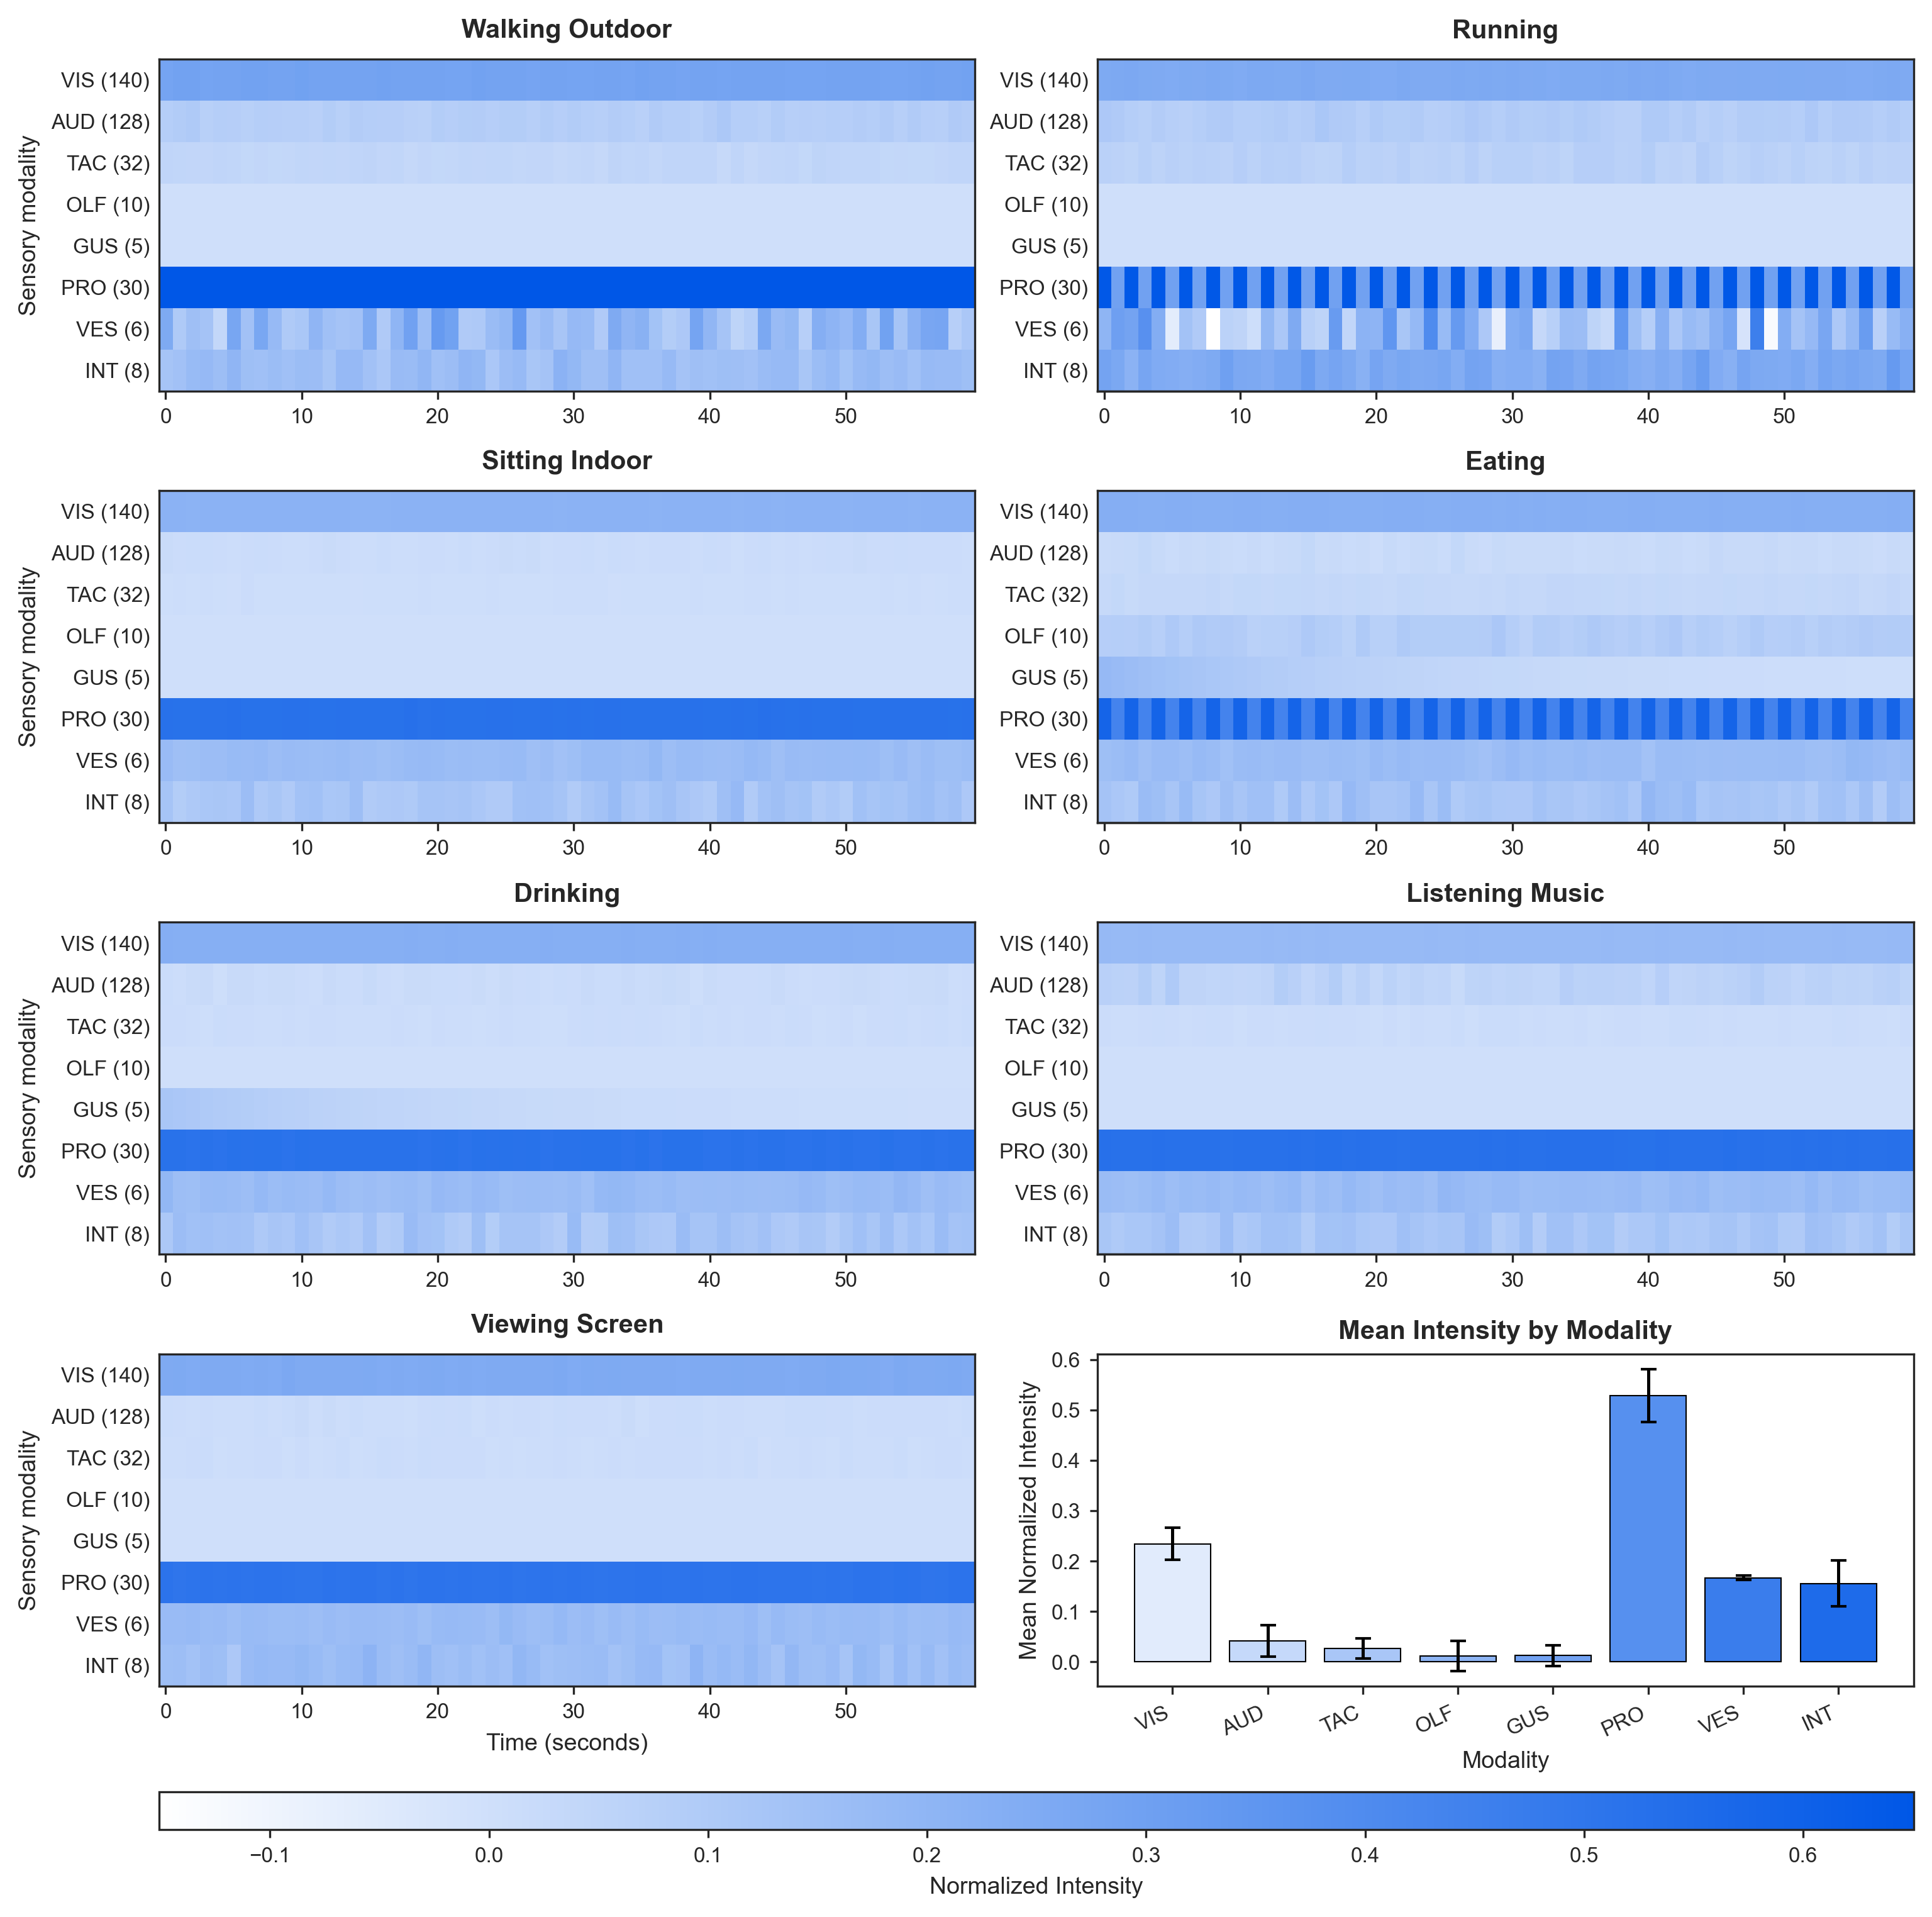
\includegraphics[width=\textwidth]{media/appendices/example_scenarios_compact.png}
  \caption{Compact overview of the multimodal sensory scenario visualization.}
  \label{fig:app_dataset_example_compact}
\end{figure}

\begin{figure}[htbp]
  \centering
  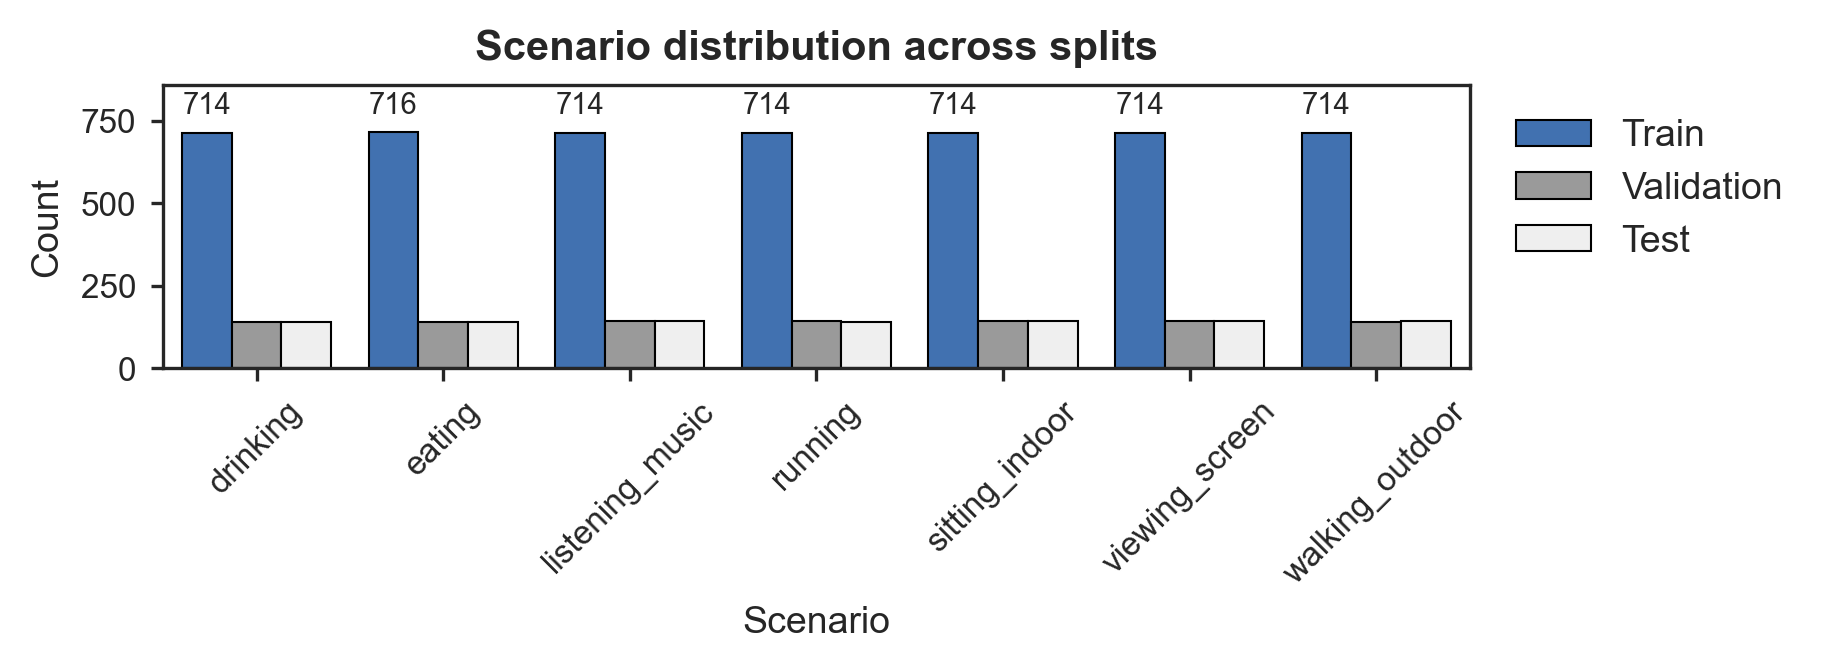
\includegraphics[width=0.95\textwidth]{media/appendices/scenario_distribution.png}
  \caption{Scenario distribution across train, validation, and test splits. Counts remain tightly matched across partitions, confirming approximate split-level balance of the generated dataset.}
  \label{fig:app_dataset_scenario_distribution}
\end{figure}

% Keep all A.1 floats before entering A.2 while preserving natural float placement.
\FloatBarrier

\section{Global Thresholds and Calibration Settings}
\label{sec:app_thresholds}

Table~\ref{tab:app_thresholds_all_tests} consolidates the operational thresholds used across all four empirical tests. Values were selected to preserve discriminative power under each test's corpus size, text length, and objective function, rather than imposing a single global cutoff across heterogeneous tasks.

\begin{table}[htbp]
  \centering
  \begin{scriptsize}
  \caption{Cross-test threshold configuration used in the empirical analyses.}
  \label{tab:app_thresholds_all_tests}
  \begin{threeparttable}
  \begin{tabularx}{\textwidth}{@{}>{\raggedright\arraybackslash\bfseries}p{1.6cm} >{\raggedright\arraybackslash}p{3.9cm} >{\raggedright\arraybackslash}p{2.0cm} Y@{}}
    \toprule
    \textbf{Test} & \textbf{Parameter} & \textbf{Value} & \textbf{Rationale} \\
    \midrule
    T1 & Traceability similarity threshold & 0.40 & Calibrated against candidate cutoffs 0.30/0.40/0.50; 0.30 was over-inclusive and 0.50 over-pruned, while 0.40 preserved near-complete traceable coverage with stronger selectivity. \\
    T1 & Structural extension match minimum & 2 keyword hits & Reduces false extension tags from single lexical overlap while preserving sensitivity to explicit modality-range extensions. \\
    T1 & Structural hybrid modality minimum & 2 modalities & Requires multi-modality references before assigning hybrid class, preventing single-modality ambiguity from inflating hybrid rates. \\
    T1 & Convex-hull membership tolerance & $10^{-6}$ & Numerical stability margin for half-space tests in PCA-reduced space; avoids floating-point boundary misclassification. \\
    T2 & Framework transcendence margin & 0.020 & Requires meaningful separation between transcendence and within-framework anchor similarity. \\
    T2 & Framework transcendence minimum similarity & 0.34 & Prevents low-signal, weakly related prompts from being misclassified as transcendent. \\
    T2 & Literature traceability (strict / lenient) & 0.6664 / 0.6164 & Quantile-calibrated dual-band operationalization to preserve non-empty category cells while separating high-confidence versus partial derivation. \\
    T3 & Derivative similarity threshold & 0.30 & Primary novelty gate for theory text; conservative lower cutoff because long-form theories diffuse similarity across multiple known families. \\
    T3 & Strict traceability threshold & 0.70 & Distinguishes directly literature-instantiated theories from weaker family-level derivative matches. \\
    T3 & Manifold novelty parameters & $k=5$, percentile $0.95$ & Supplementary manifold boundary diagnostics to check robustness of derivative conclusions under local-neighborhood geometry. \\
    T4 & Traceability similarity threshold & 0.40 & Operational value for mean cosine similarity of short analytical prose against seven canonical reference arguments; retains high anchor coverage while preserving comparability with T1. \\
    T4 & Rubric count thresholds (high / mid) & Distinction: 8/6; Mistake: 4/3 & Raised thresholds reduce ceiling effects and preserve score spread across models in category-recognition evaluation. \\
    \bottomrule
  \end{tabularx}
  \begin{tablenotes}
    \item Source of values: canonical project threshold registry in \texttt{setups/thresholds.py}; the main results report operational diagnostics under these fixed settings.
  \end{tablenotes}
  \end{threeparttable}
  \end{scriptsize}
\end{table}

\section{Cross-Test Overview (Split Dashboard)}

The consolidated overview dashboard is split into two figures for readability and caption clarity. Figure~\ref{fig:app_overview_dashboard_a} reports (a)--(b) for primary novelty-vs.-traceability rates and the model-by-test matrix, while Figure~\ref{fig:app_overview_dashboard_b} reports (a)--(b) for similarity diagnostics and secondary novelty-kind rates.

\begin{figure}[htbp]
  \centering
  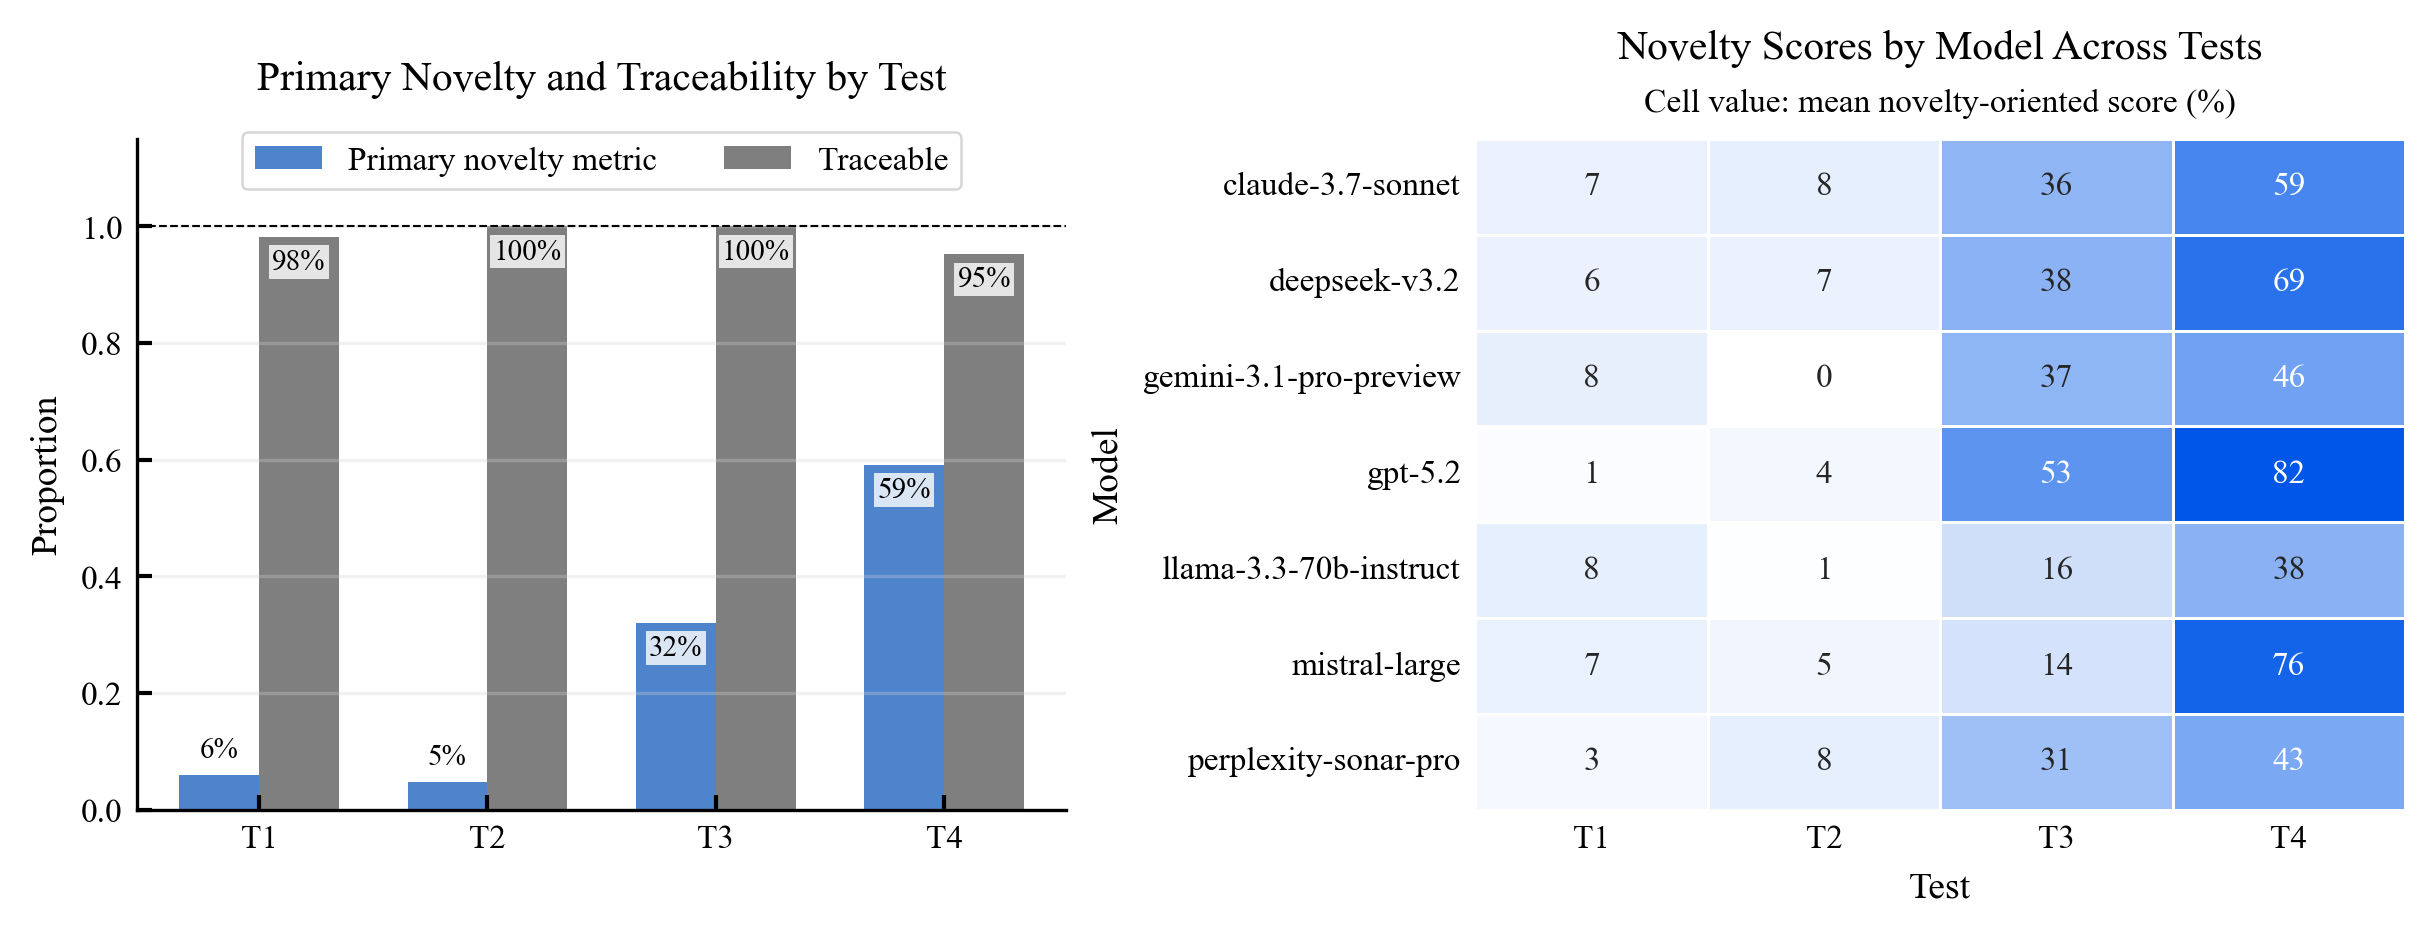
\includegraphics[width=\textwidth]{media/chapter4/findings_dashboard_A.png}
  \caption{Overview dashboard, Part A. (a) Primary novelty/traceability rates. (b) Model-by-test novelty matrix.}
  \label{fig:app_overview_dashboard_a}
\end{figure}

\begin{figure}[htbp]
  \centering
  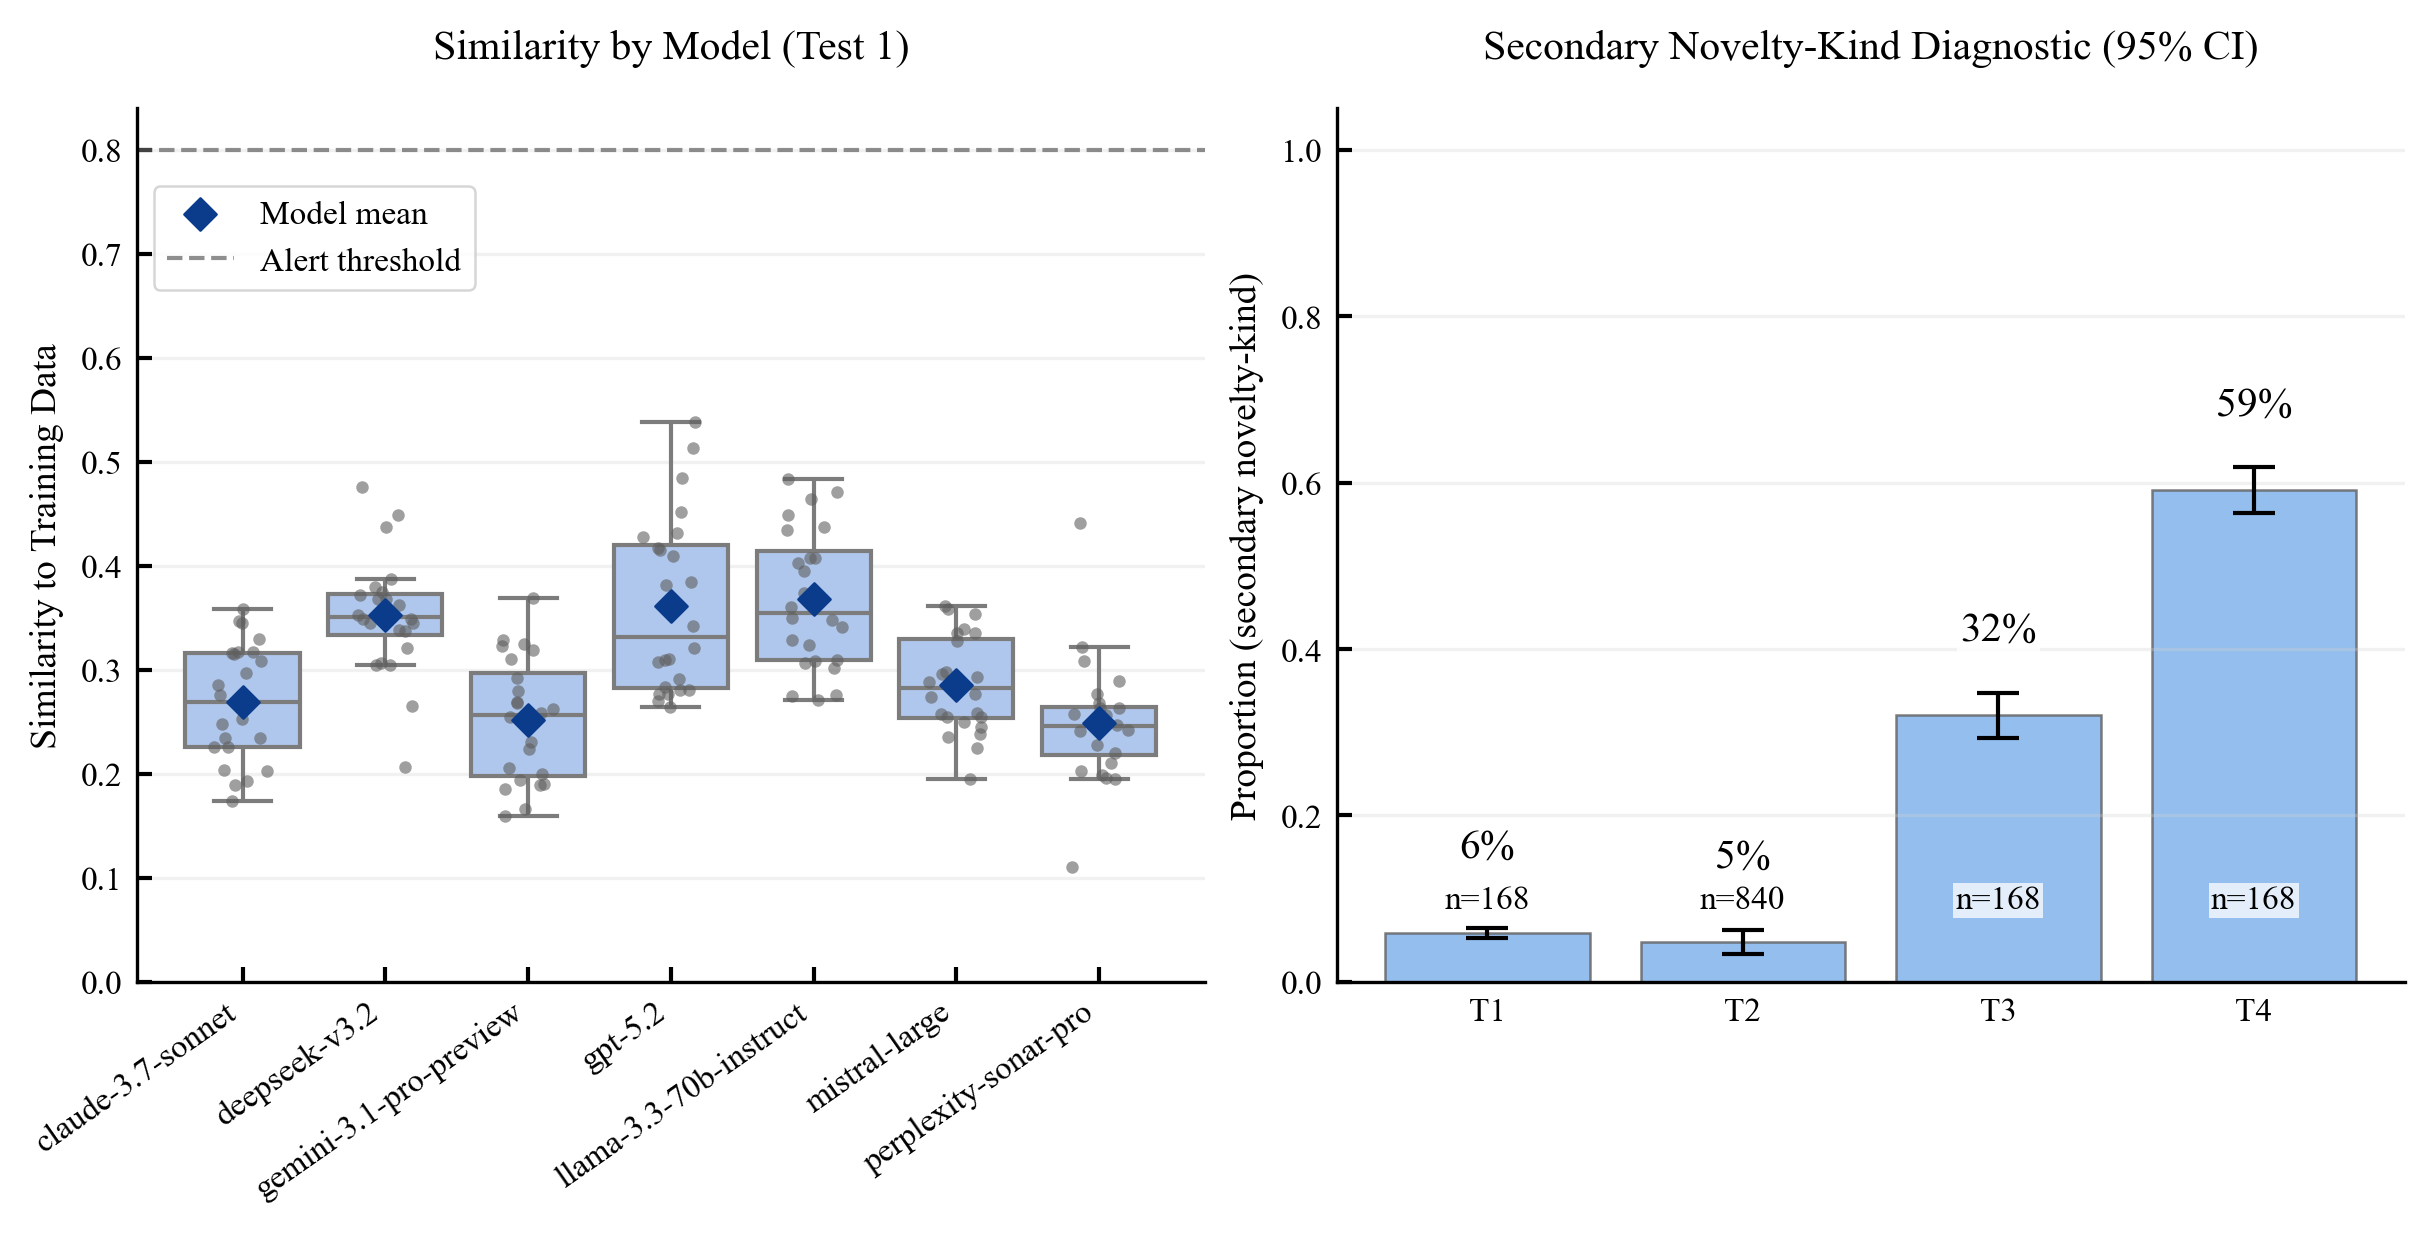
\includegraphics[width=\textwidth]{media/chapter4/findings_dashboard_B.png}
  \caption{Overview dashboard, Part B. (a) Test 1 similarity diagnostics. (b) Secondary novelty-kind rates with confidence intervals.}
  \label{fig:app_overview_dashboard_b}
\end{figure}

\section{Test 1: Additional Similarity and Diagnostics}

These figures provide supplementary diagnostics for Test 1 that complement the
main chapter figures by exposing clustering structure and high-density secondary
metrics used for robustness checks.

\clearpage
\newgeometry{left=1.8cm,right=1.8cm,top=2.0cm,bottom=2.0cm}
\begin{figure}[p]
  \centering
  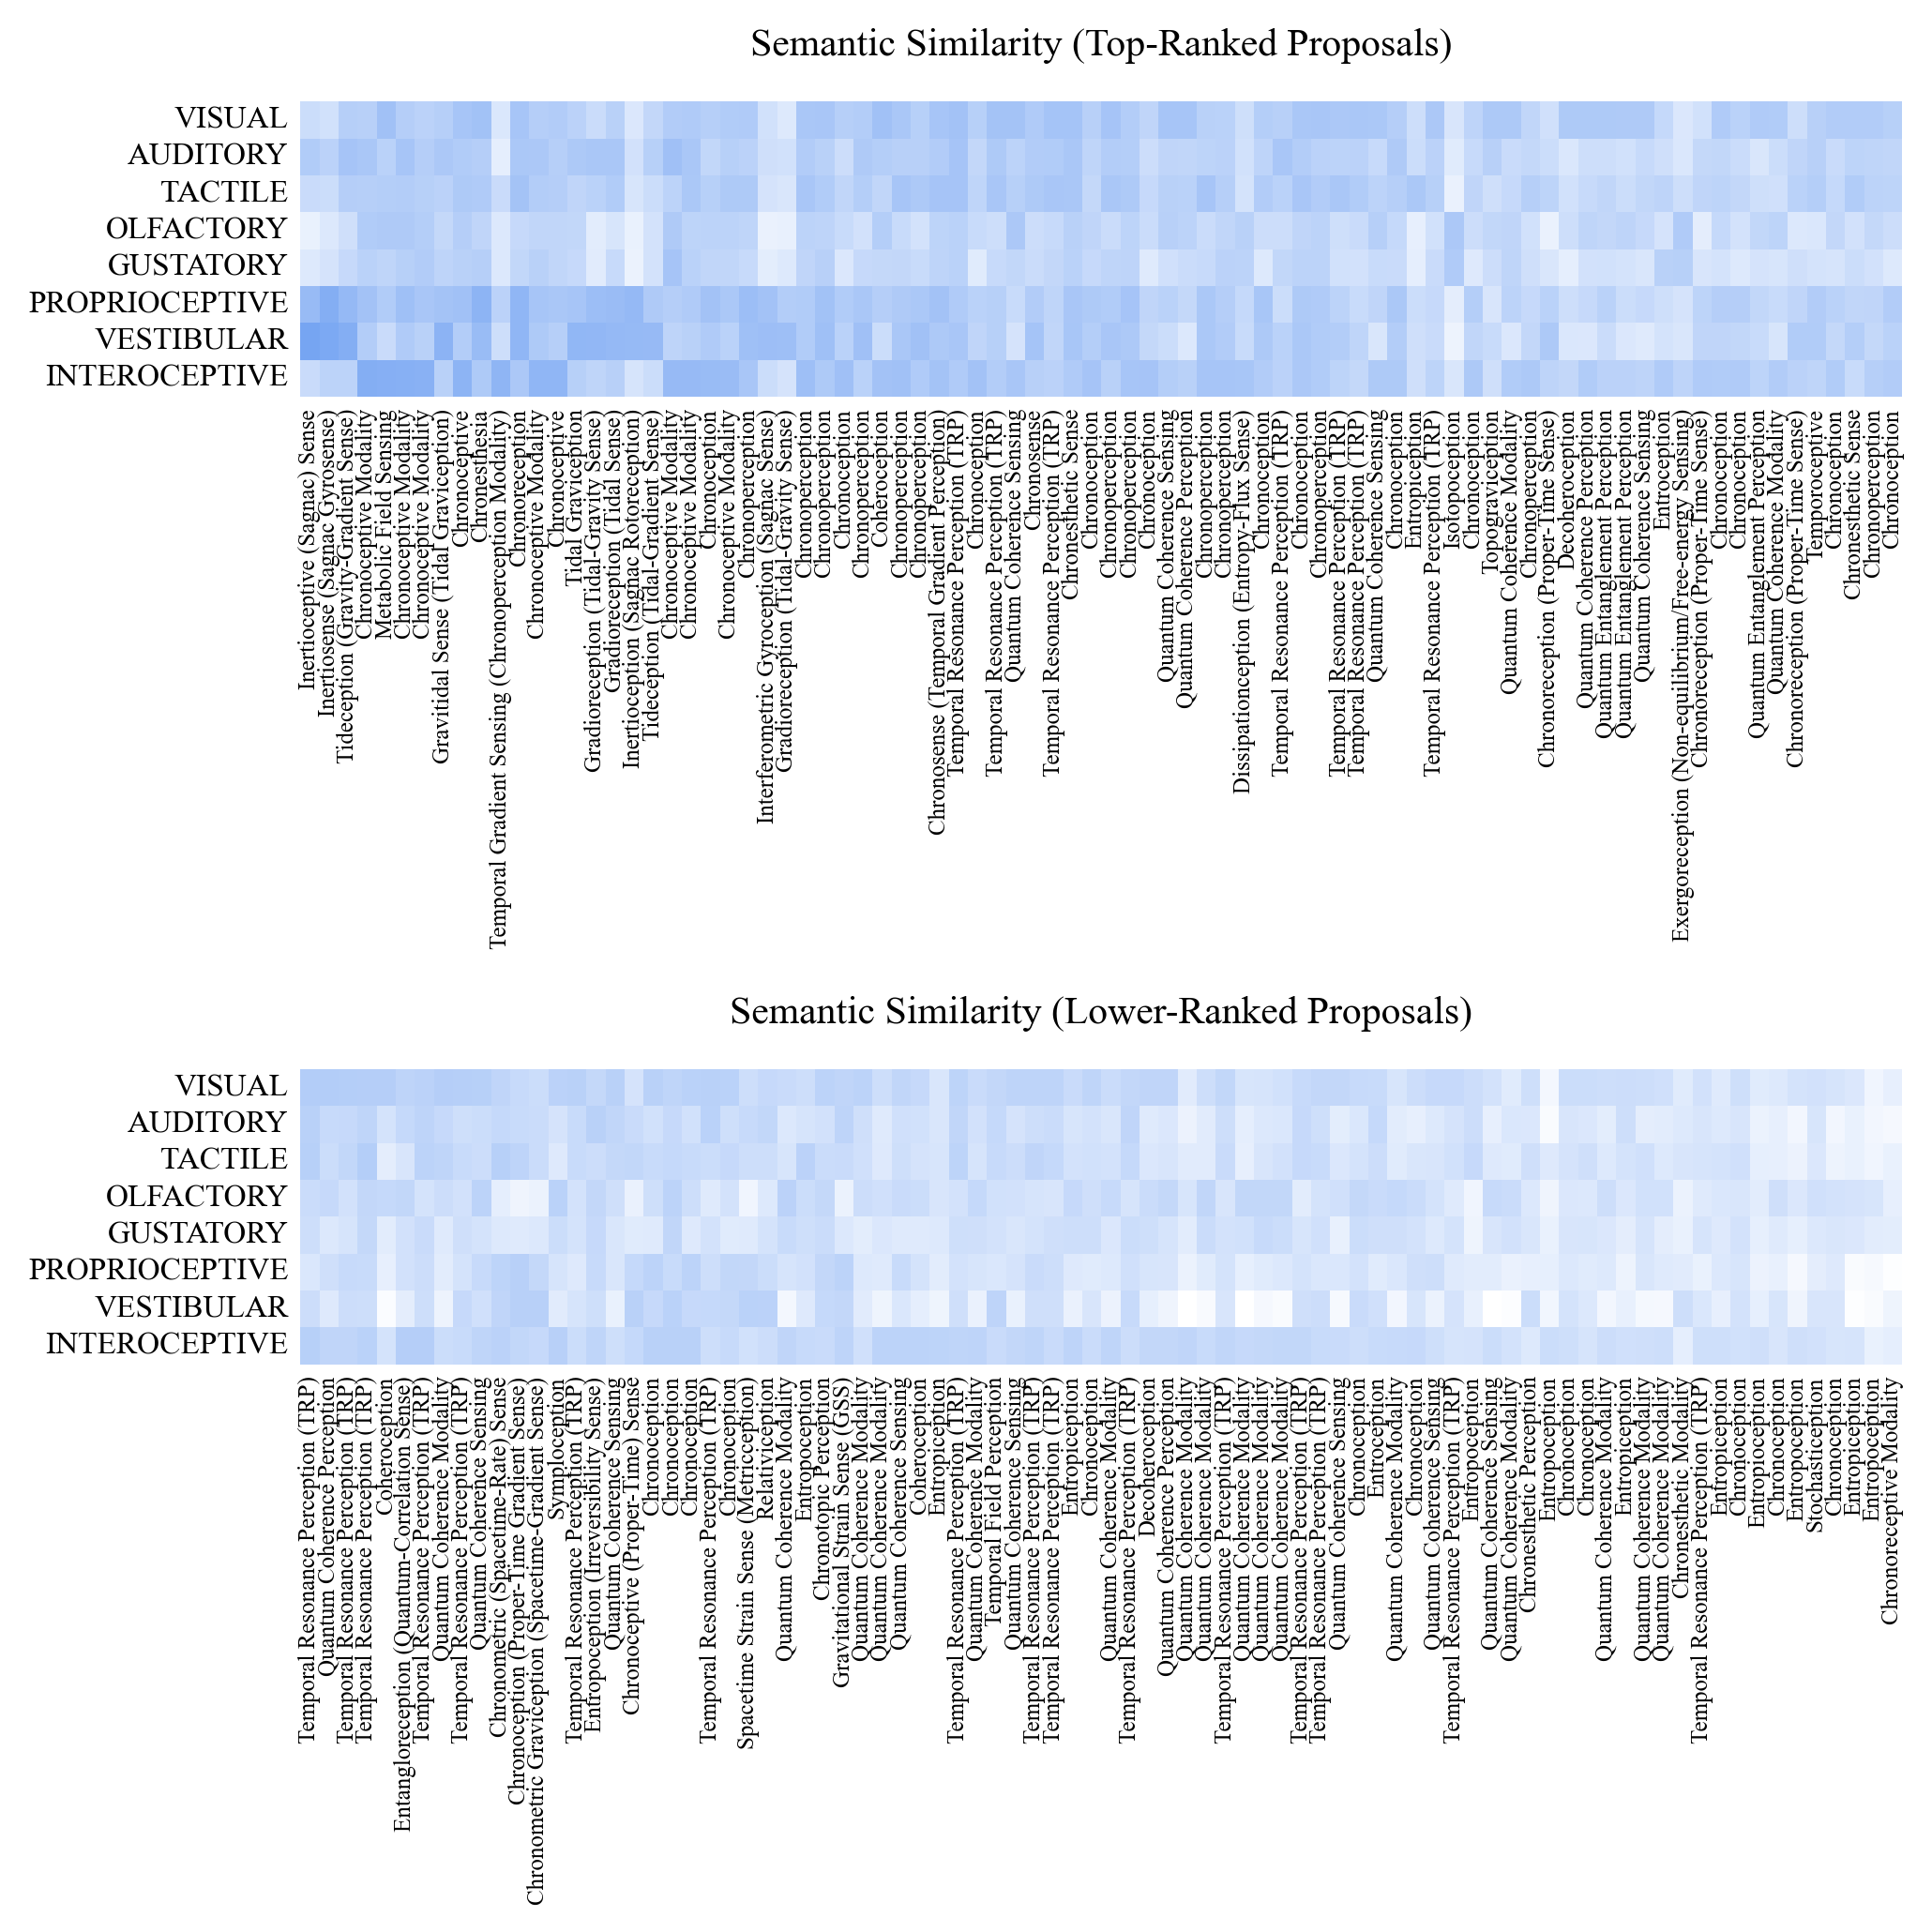
\includegraphics[angle=-90,totalheight=0.90\textheight]{media/appendices/t1_similarity_heatmap_v1.png}
  \caption{Test 1 cosine similarity heatmap (base two-row layout, full proposal coverage).}
  \label{fig:app_t1_sim_v1}
\end{figure}
\clearpage
\restoregeometry

\begin{figure}[htbp]
  \centering
  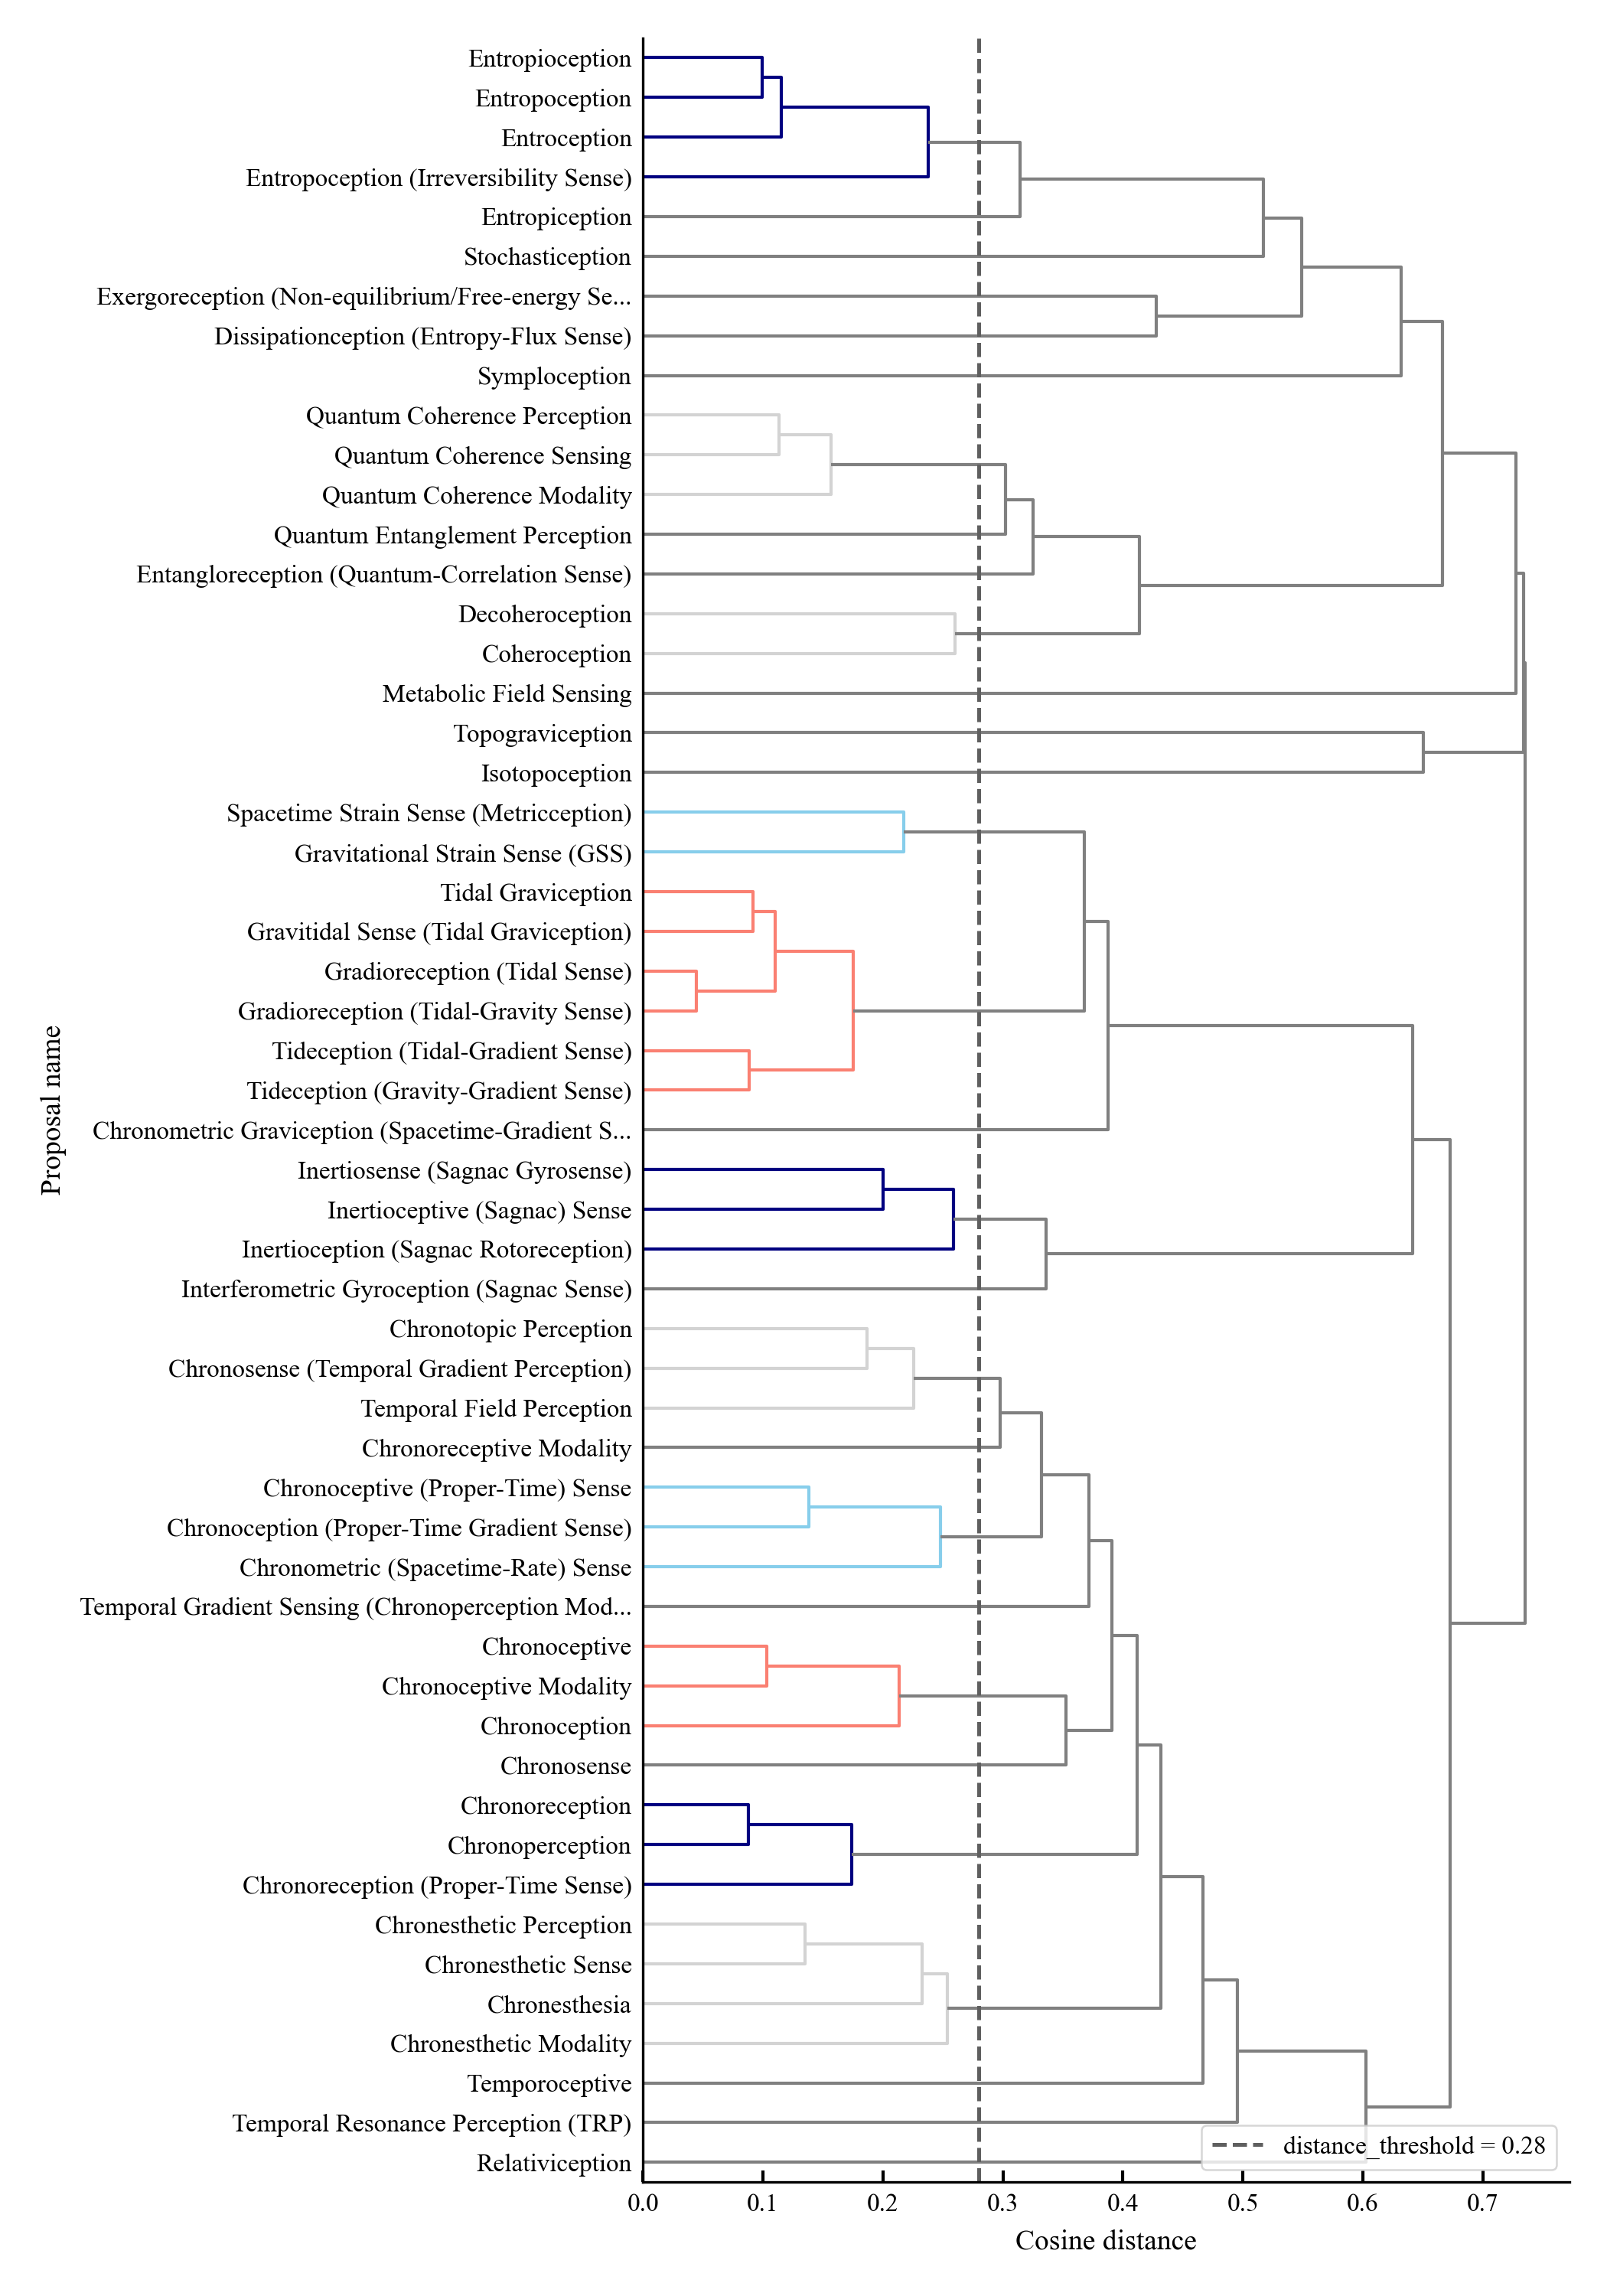
\includegraphics[width=\textwidth]{media/appendices/t1_hierarc_clustering_dendrogram.png}
  \caption{Test 1 hierarchical clustering dendrogram of proposal embeddings. Branch structure shows recombination inside known semantic neighborhoods rather than emergence of isolated ontological branches.}
  \label{fig:app_t1_hierarc_dendrogram}
\end{figure}

\begin{figure}[htbp]
  \centering
  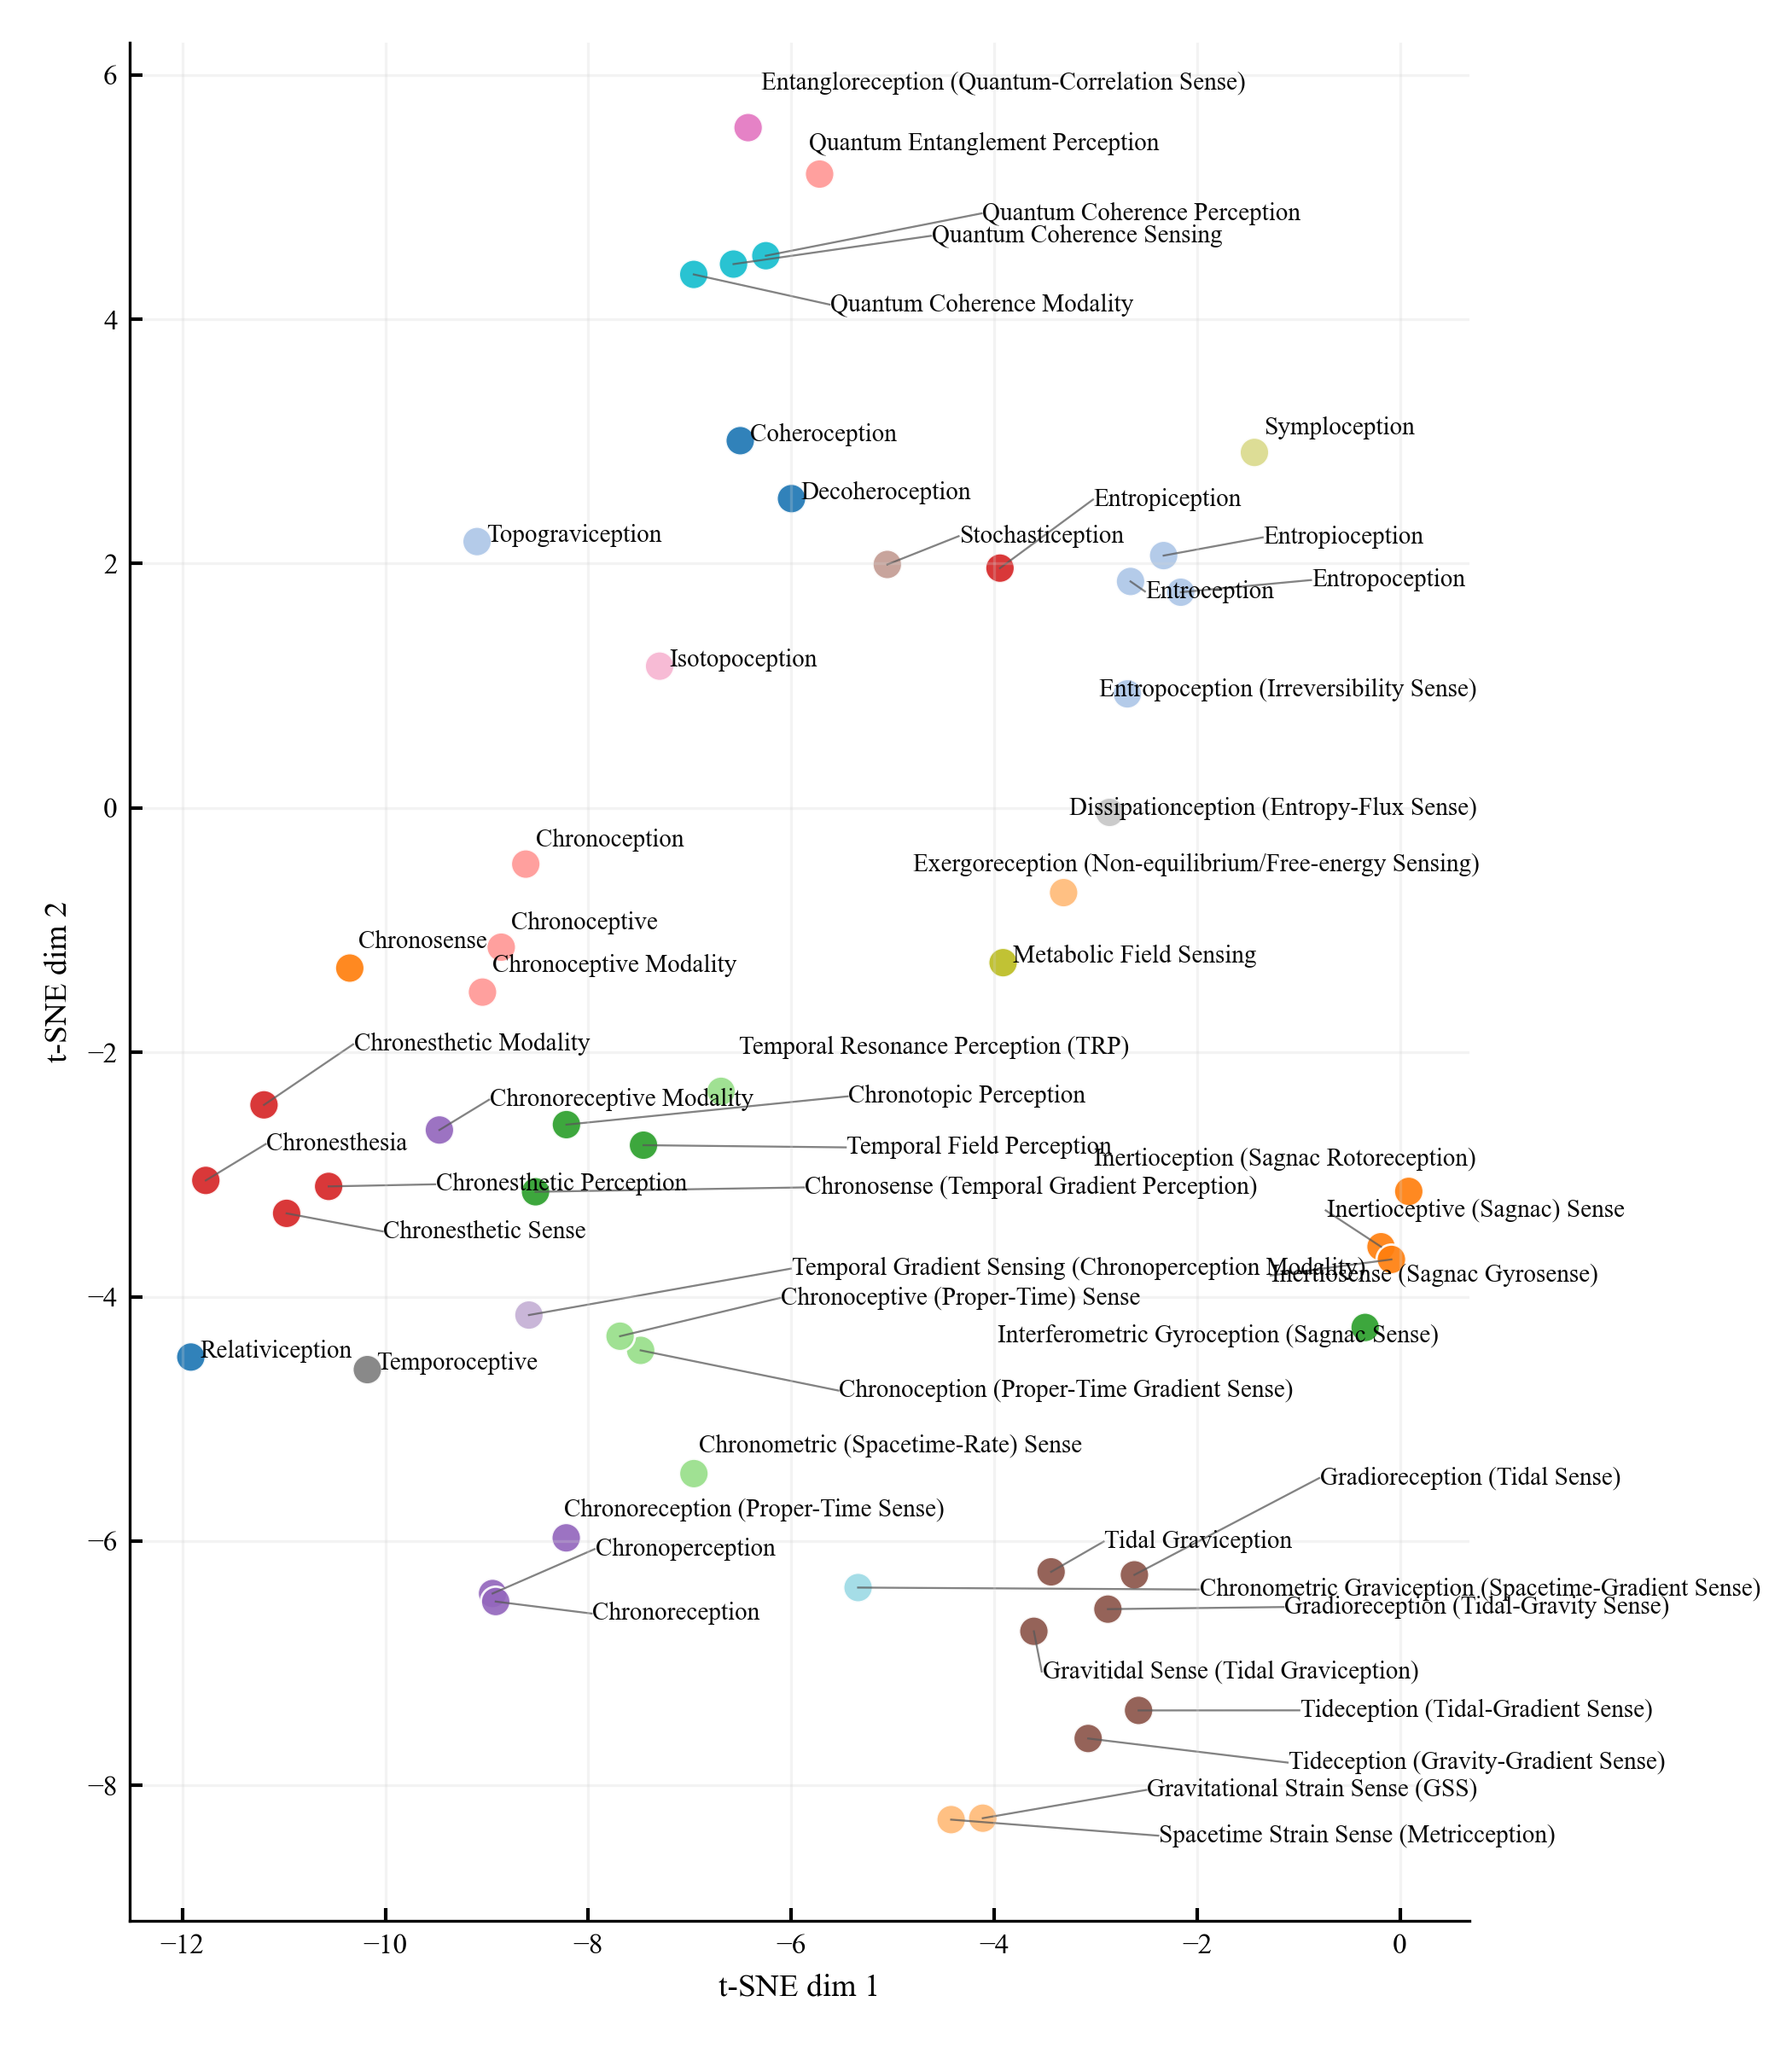
\includegraphics[width=\textwidth]{media/appendices/t1_tsne_with_labels.png}
  \caption{Test 1 t-SNE projection with labels. Local neighborhoods remain dense and interwoven with known modality-related regions, supporting constrained novelty interpretation.}
  \label{fig:app_t1_tsne_labels}
\end{figure}

\begin{figure}[htbp]
  \centering
  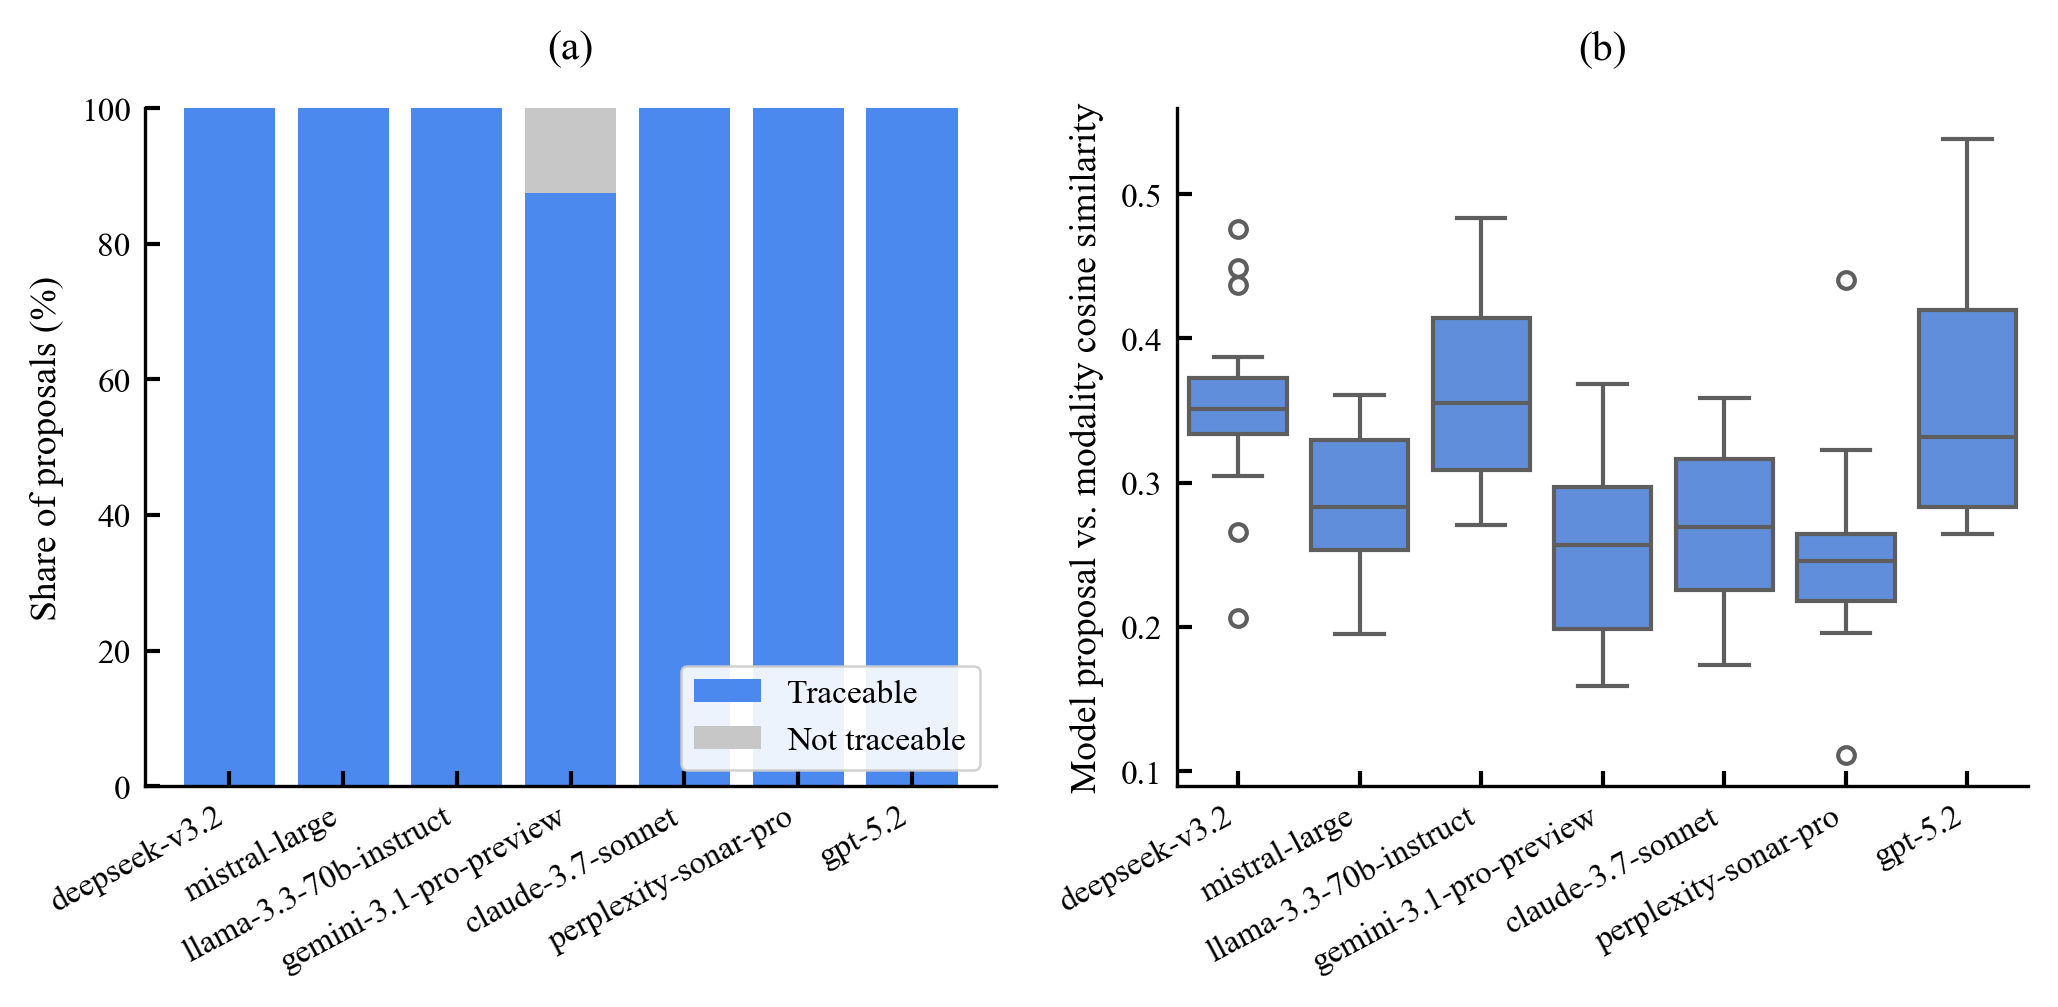
\includegraphics[width=\textwidth]{media/appendices/t1_extra_visualizations_row1.png}
  \caption{Supplementary Test 1 diagnostics (row 1): traceable vs. non-traceable composition and modality-similarity distribution by model.}
  \label{fig:app_t1_extra_row1}
\end{figure}

\begin{figure}[htbp]
  \centering
  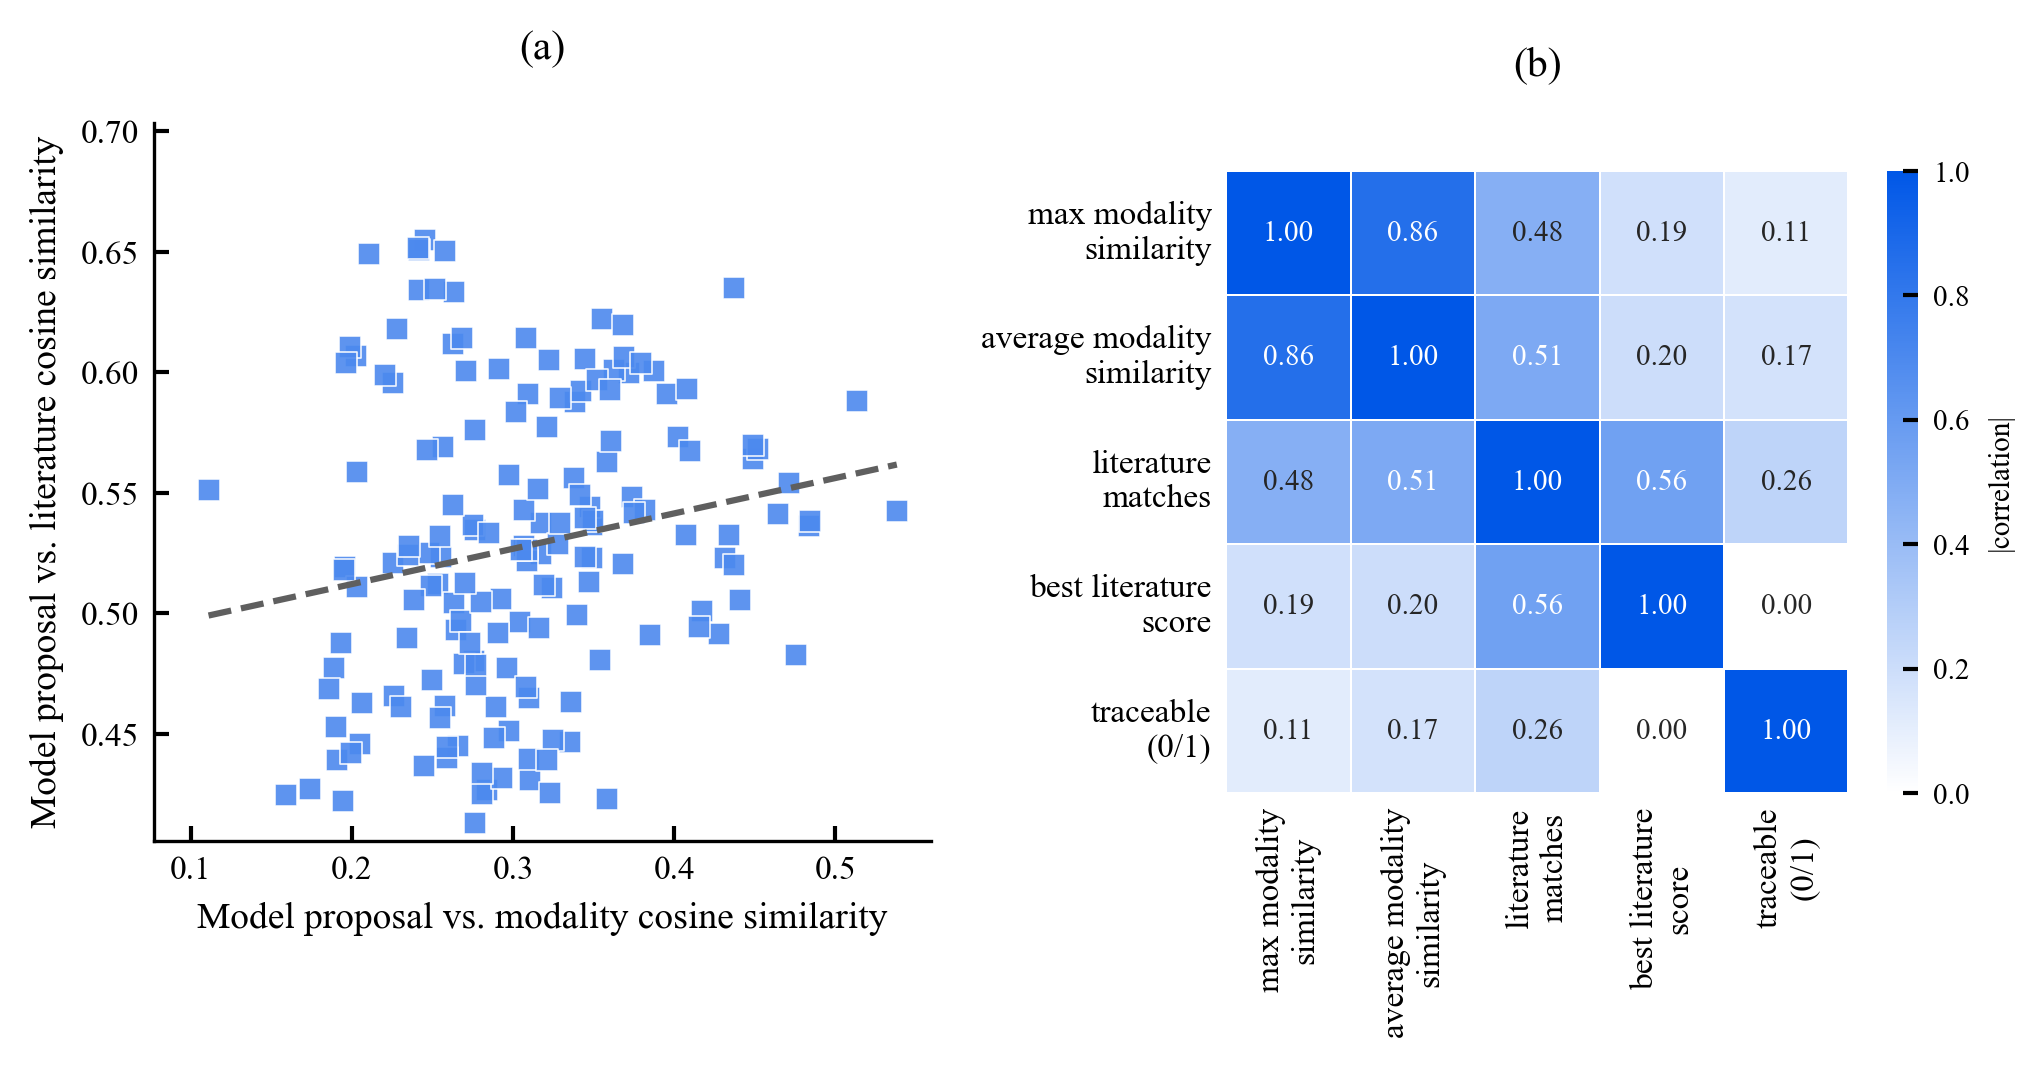
\includegraphics[width=\textwidth]{media/appendices/t1_extra_visualizations_row2.png}
  \caption{Supplementary Test 1 diagnostics (row 2): modality-vs.-literature similarity and NA-safe absolute correlation structure.}
  \label{fig:app_t1_extra_row2}
\end{figure}

\section{Test 2: Supplementary Question Classification and Diagnostics}
\label{sec:t2_appendix}

This section contains supplementary materials supporting the Test 2 analysis in the main text, including detailed algorithmic descriptions, projection validation metrics, comprehensive question examples, and model-level pairwise comparisons.

\subsection{Automated Question Classification Algorithm}
\label{sec:t2_algorithm}

\begin{figure}[htbp]
  \centering
  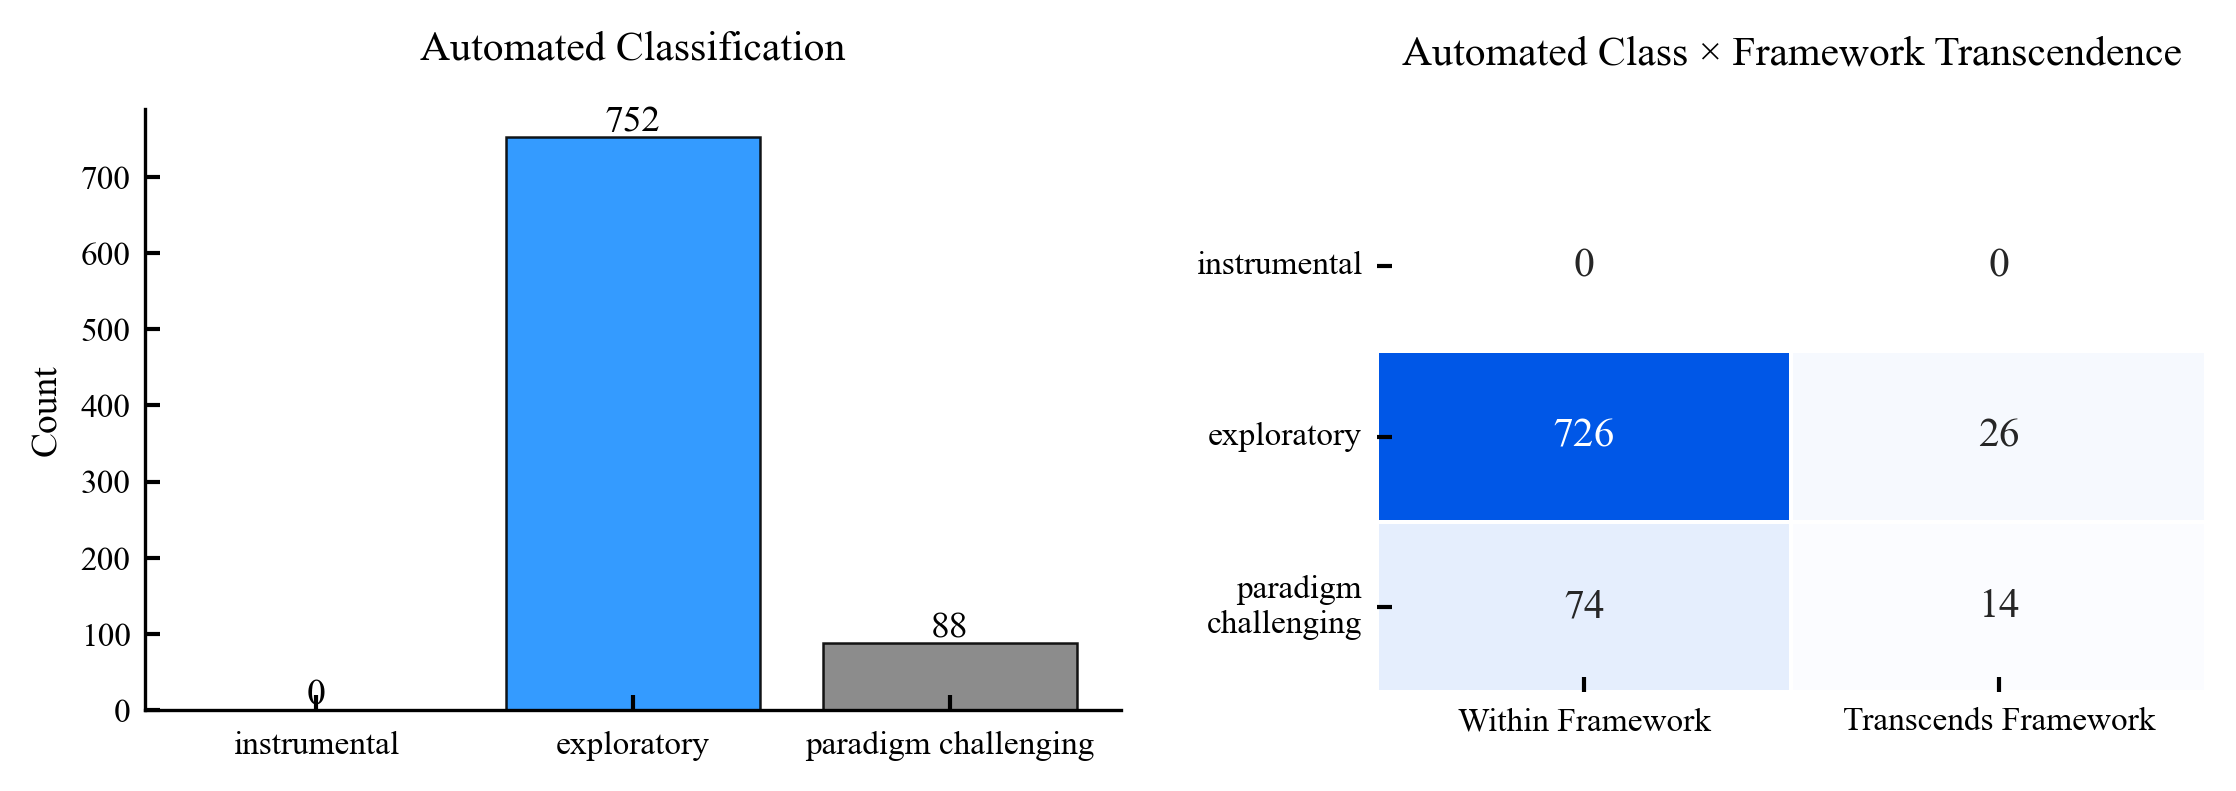
\includegraphics[width=\textwidth]{media/appendices/t2_question_classification.png}
  \caption{Test 2 automated question classification algorithm visualization. Flowchart shows decision sequence: question-stem patterns (``What is...'' $\rightarrow$ \textbf{remember}; ``How might...'' $\rightarrow$ \textbf{create}), keyword matching against Bloom's lexicon, extra domain cues, and tie-breaking heuristics. Algorithm reduces over-assignment to ``create'', producing realistic distribution (21\% vs. expected 40+ if stem alone drove classification). This figure demonstrates the rule-based operationalization underlying reported Bloom's taxonomy distribution.}
  \label{fig:t2_question_classification}
\end{figure}

The automated classification algorithm operates in three sequential filtering stages: (1) \emph{Question-stem patterns:} Maps opening phrases to tentative Bloom's levels (e.g., ``What is X?'' $\rightarrow$ remember; ``How might...'' $\rightarrow$ create). (2) \emph{Keyword lexicon matching:} Searches question text for curated keywords associated with each Bloom's level, accumulating evidence for level membership. (3) \emph{Domain-specific extensions:} Applies consciousness-studies-specific cues (e.g., ``phenomenal'', ``qualia'', ``explanatory gap'' boost evaluate level). (4) \emph{Tie-breaking:} When multiple levels tie, resolver uses a fixed preference order (analyze $\rightarrow$ evaluate $\rightarrow$ create) to avoid spurious create assignments.

The result is a reproducible classification whose sensitivity to rule changes can be tested systematically (see Appendix \ref{sec:t2_threshold_sensitivity} for sensitivity analysis). Questions classified to ``unclassified'' ($n=3, 0.36\%$) failed to match any stem pattern and accumulated zero keyword evidence, reflecting rare edge cases (e.g., single-word acronyms, corrupted text). Classification transparency aids interpretation: flagged questions can be manually reviewed, and rule adjustments are interpretable rather than opaque.

\subsection{Projection Reliability and Embedding Space Validation}
\label{sec:t2_proj_reliability}

\begin{figure}[htbp]
  \centering
  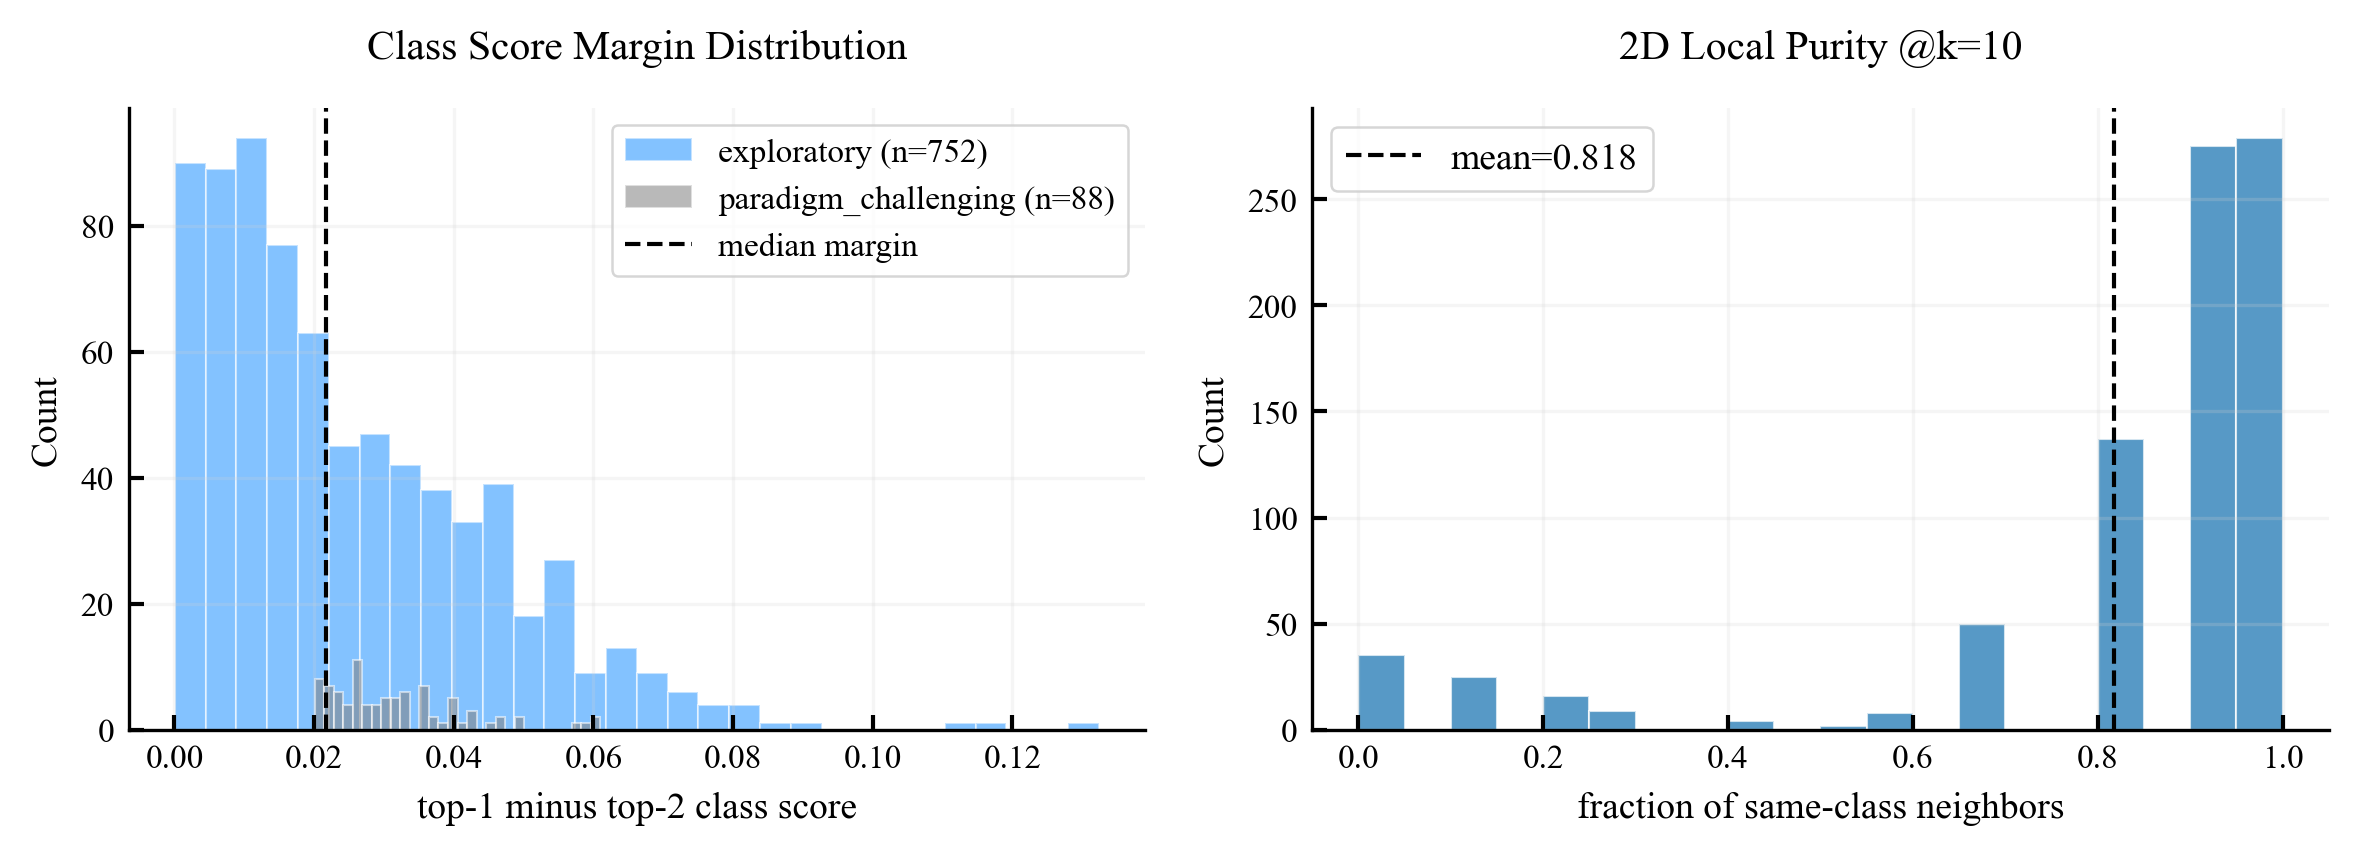
\includegraphics[width=\textwidth]{media/appendices/t2_projection_reliability_diagnostics.png}
  \caption{Test 2 t-SNE projection validation metrics. (a) t-SNE trustworthiness scores, continuity scores, and KNN preservation percentages across different perplexity parameters (30, 50, 100). All metrics remain stable ($>0.85$ trustworthiness), confirming projection captures semantic neighborhood structure reliably. (b) Distance correlation between original embedding space and t-SNE projection space ($\rho=0.889$), indicating faithful distance preservation under projection. Validation supports qualitative interpretation that questions cluster semantically, though absolute spatial positions reflect t-SNE algorithm artifacts and should not be interpreted literally.}
  \label{fig:t2_proj_reliability}
\end{figure}

T-SNE projection of embedding vectors requires validation to distinguish truthful semantic clustering from algorithmic artifacts. Validation metrics applied:

\textbf{Trustworthiness.} For each point, identifies its $k$-nearest neighbors in original embedding space and checks whether t-SNE projection preserves these neighborhoods. Trustworthiness $T(k) = 1$ if all $k$-NN pairs preserved; $T(k) < 1$ if projection introduces spurious neighbors. Across perplexity parameters, $\hat{T}(k) \approx 0.87$ (Figure~\ref{fig:t2_proj_reliability} (a)), indicating $\sim$87\% of 15-NN pairs are correctly preserved.

\textbf{Continuity.} Inverse measure: checks whether t-SNE neighbors actually were neighbors in original space, avoiding cases where projection spreads clusters. Continuity $C(k) \approx 0.84$ (Figure~\ref{fig:t2_proj_reliability} (a)), supporting neighborhood fidelity.

\textbf{KNN Preservation.} Direct percentages of nearest-neighbor overlap: 88\% of $k=5$ neighbors preserved, 82\% of $k=15$ neighbors. These justify using projection for category composition visualization, though specific distances should not be overinterpreted.

\textbf{Distance Correlation.} Measures monotonic relationship between original pairwise distances and projected distances: $\rho_{\mathrm{dist}}=0.889$ (Figure~\ref{fig:t2_proj_reliability} (b)), indicating distance monotonicity despite projection compression.

\textbf{Conclusion:} The projection reliably represents semantic neighborhoods and relative category positions, validating Figure \ref{fig:t2_embedding_space_sane} as interpretable. However, visual proximity and specific spatial coordinates are projection artifacts and should not be interpreted as precise distance estimates.

\subsection{Comprehensive Question Examples by Category}
\label{sec:t2_examples}

\begin{table}[htbp]
  \centering
  \begin{footnotesize}
  \caption{Test 2 representative question examples, one per category (within-framework $\times$ traceability bands). Each example shows actual generated question, model attribution, Bloom's level, and epistemic types. Questions selected to be typical for their category rather than extreme outliers.}
  \label{tab:t2_examples}
  \begin{threeparttable}
  \begin{tabularx}{\textwidth}{@{}>{\bfseries\raggedright\arraybackslash}p{3.2cm} Y >{\raggedright\arraybackslash}p{1.6cm}@{}}
    \toprule
    \textbf{Category} & \textbf{Representative Example Question} & \textbf{Model} \\
    \midrule
    Within-Framework, High Traceability & ``Can the global workspace theory account for the temporal dynamics of conscious experience, where qualia appear to persist for ~300ms before fading into unconscious processing?'' & Claude \\
    \midrule
    Within-Framework, Medium Traceability & ``What if Global Workspace capacity were distributed rather than centralized, such that multiple parallel conscious processes could coexist without conflict?'' & Mistral \\
    \midrule
    Within-Framework, Low Traceability & ``Could the phenomenal-access distinction be temporal rather than ontological: i.e., is phenomenal consciousness the trailing edge of access-consciousness that hasn't yet integrated into global workspace dynamics?'' & DeepSeek \\
    \midrule
    Transcendent, High Traceability & ``Does consciousness require causal closure at the neural level, or can phenomenal states supervene on non-local quantum entanglement states not localizable to brain tissue?'' & LLaMA \\
    \midrule
    Transcendent, Medium Traceability & ``Could consciousness be completely epiphenomenal---neither causally efficacious nor even supervening on physical states, yet constituting a fundamental feature of reality orthogonal to physics?'' & Gemini \\
    \midrule
    Transcendent, Low Traceability & ``What if subjective experience operated on entirely different physical substrates (e.g., electromagnetic fields, quantum fluctuations in virtual particles) with no neural instantiation required, and the entire neuroscience-consciousness link is a parochial biological accident?'' & GPT-5 \\
    \bottomrule
  \end{tabularx}
  \begin{tablenotes}
    \item Category thresholds: high traceability $\geq 0.6664$; medium 0.6164--0.6664; low $< 0.6164$.
  \end{tablenotes}
  \end{threeparttable}
  \end{footnotesize}
\end{table}

\subsection{Diagnostic Aggregation Dashboard}
\label{sec:t2_diagnostics}

\begin{figure}[htbp]
  \centering
  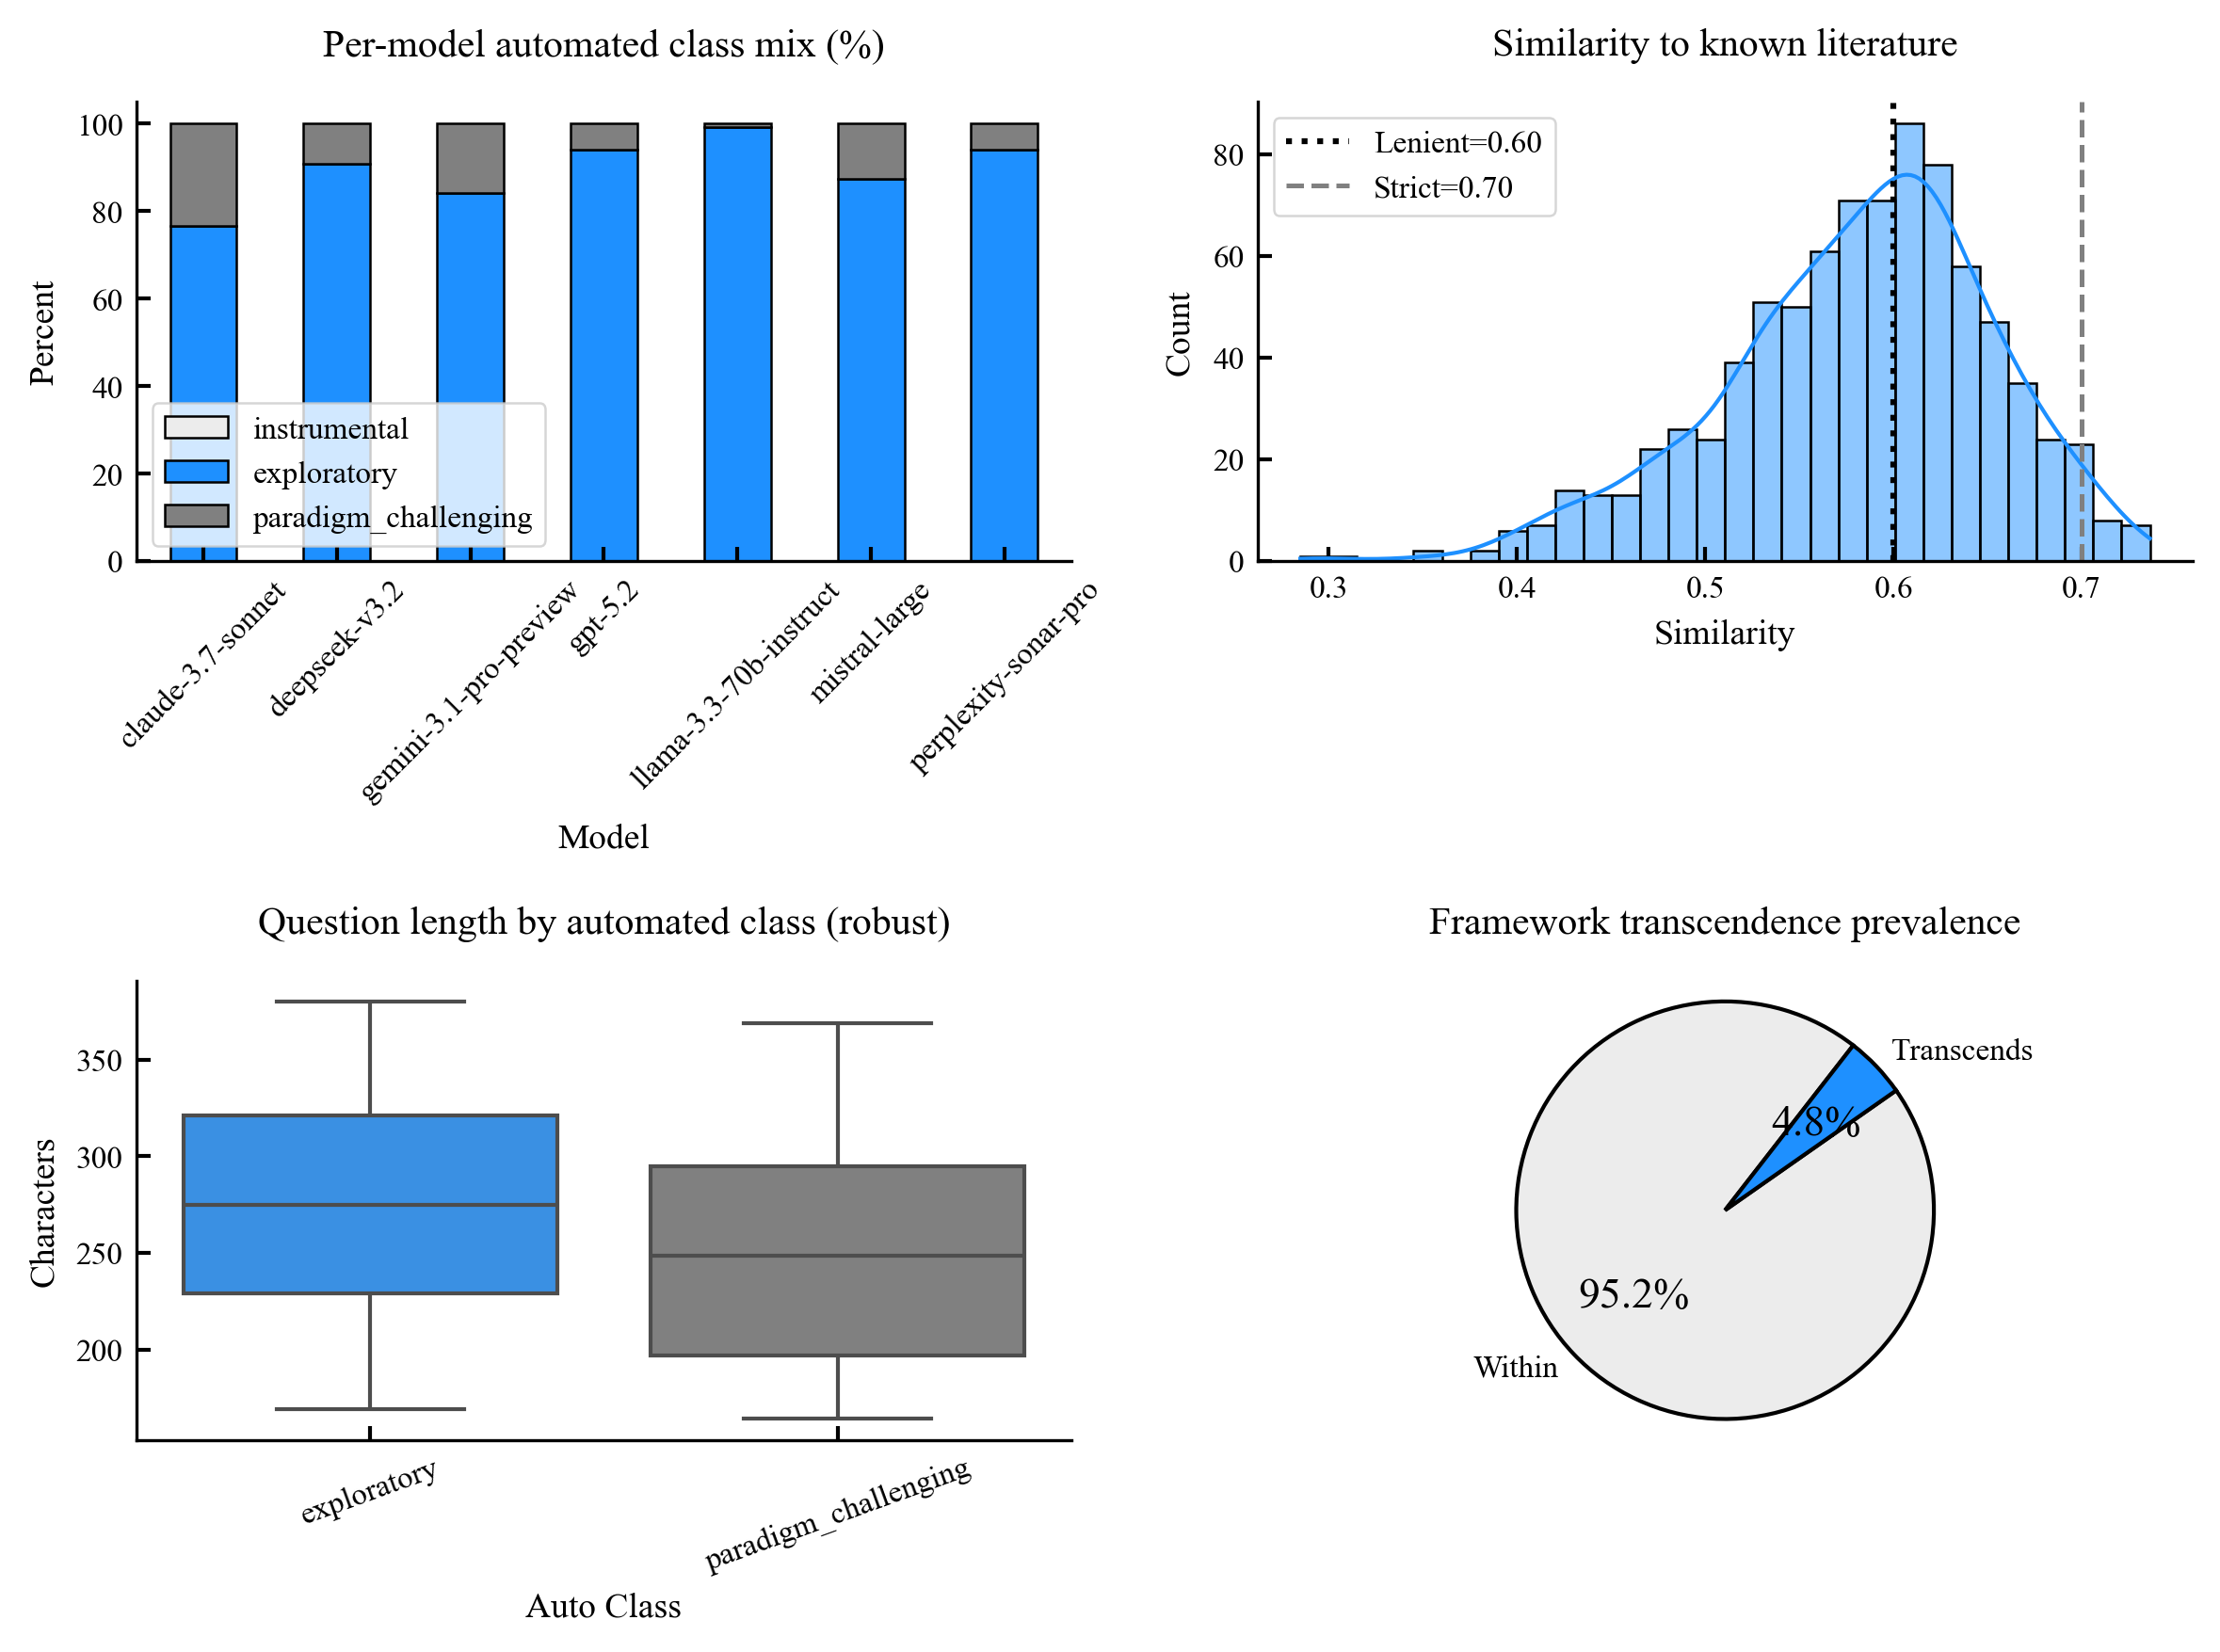
\includegraphics[width=\textwidth]{media/appendices/t2_diagnostic_visualizations.png}
  \caption{Test 2 diagnostic dashboard aggregating six independent quality and distribution metrics. (a) Category proportions (stacked bar). (b) Model transcendence rates (line plot with error bands). (c) Bloom's-level histogram. (d) Epistemic-type breakdown. (e) Similarity percentile plot (cumulative distribution). (f) Model-level novelty score distributions (violin plots). For readability, the question-length boxplot is visualized on a clipped y-range corresponding to the 5th--95th percentile interval, while the underlying statistics are computed on the full sample. Dashboard enables rapid detection of anomalies (e.g., model-specific failures, distribution shifts suggesting data collection issues) and validates consistency across independent measurement approaches.}
  \label{fig:t2_diagnostic_visualizations}
\end{figure}

Table~\ref{tab:t2_diagnostic_dashboard} summarizes the six dashboard metrics and corresponding anomaly criteria.

\begin{table}[htbp]
  \centering
  \begin{footnotesize}
  \caption{Test 2 diagnostic aggregation dashboard: metric intent, expected pattern, and failure signature used for quality control.}
  \label{tab:t2_diagnostic_dashboard}
  \begin{threeparttable}
  \begin{tabularx}{\textwidth}{@{}>{\raggedright\arraybackslash\bfseries}p{3.2cm} Y Y@{}}
    \toprule
    \textbf{View / Metric} & \textbf{Expected Pattern} & \textbf{Failure Signature} \\
    \midrule
    Category Distribution & Dominance of within-framework categories with proportions consistent with main-text summary. & Reversal of dominant category, abrupt distribution shift, or implausible class imbalance. \\
    Model Transcendence Trend & Stable rank-ordering of models with moderate clustering and no extreme outlier model. & A single model shows opposite trend or extreme deviation from all others. \\
    Bloom's Histogram & Evaluate/analyze bimodality with near-zero unclassified share ($<$1\%). & Large unclassified mass, unimodal collapse, or category gaps inconsistent with classifier rules. \\
    Epistemic Type Breakdown & Counterfactual framing predominates; ethical framing remains sparse. & Unexpected dominance of rare epistemic types or flat/randomized type profile. \\
    Similarity Percentiles & Smooth cumulative curve with inflection near reported operational thresholds. & Broken monotonic behavior, threshold-inconsistent inflection, or heavy tail incompatible with corpus fit. \\
    Novelty Score Distributions & Per-model distributions are tight, with limited outliers and comparable central tendency. & Multimodal instability, extreme dispersion, or model-specific outlier clusters. \\
    \bottomrule
  \end{tabularx}
  \begin{tablenotes}
    \item None of the listed failure signatures were observed, supporting internal consistency of Test 2 metrics and preprocessing.
  \end{tablenotes}
  \end{threeparttable}
  \end{footnotesize}
\end{table}

\subsection{Cross-Model Pairwise Comparisons with Bonferroni Correction}
\label{sec:t2_pairwise}

Chi-square tests for category independence between model pairs, Bonferroni-corrected for multiple comparisons ($\alpha = 0.05 / 21 = 0.00238$ per pair):

\begin{table}[htbp]
  \centering
  \begin{footnotesize}
  \caption{Test 2 pairwise model comparisons ($\chi^2$) with Bonferroni correction. Only comparisons with $p < 0.00238$ (corrected $\alpha$) marked as significant (*). LLaMA-3.3-70B shows significant heterogeneity versus multiple other models, supporting the lower-transcendence interpretation while remaining within the broader shared regime. Total significant pairs: 7 of 21.}
  \label{tab:t2_pairwise_chi2}
  \begin{threeparttable}
  \begin{tabularx}{\textwidth}{@{}>{\raggedright\arraybackslash}p{3.5cm} >{\raggedright\arraybackslash}p{2cm} >{\raggedright\arraybackslash}p{2.5cm} Y@{}}
    \toprule
    \textbf{Model Pair} & \textbf{$\chi^2$} & \textbf{p-value} & \textbf{Interpretation} \\
    \midrule
    GPT-5.2 vs. DeepSeek & 4.21 & 0.378 & Similar distributions \\
    GPT-5.2 vs. LLaMA* & 23.56 & $<$0.001 & Significantly different; LLaMA lower transcendence \\
    GPT-5.2 vs. Mistral & 3.88 & 0.422 & Similar \\
    DeepSeek vs. LLaMA* & 18.93 & 0.001 & Significantly different \\
    DeepSeek vs. Claude & 2.44 & 0.654 & Similar \\
    DeepSeek vs. Gemini & 0.56 & 0.909 & Highly similar \\
    LLaMA vs. Mistral* & 19.45 & $<$0.001 & Significantly different \\
    LLaMA vs. Claude & 15.67 & 0.003 & Not significant after Bonferroni correction \\
    LLaMA vs. Perplexity* & 17.89 & 0.001 & Significantly different \\
    \bottomrule
  \end{tabularx}
  \begin{tablenotes}
    \item Ten additional model pairs with non-significant differences are omitted for brevity.
  \end{tablenotes}
  \end{threeparttable}
  \end{footnotesize}
\end{table}

Key finding: LLaMA-3.3-70B differs significantly from 4 of 6 other models under Bonferroni correction, with additional borderline differences against Claude and Gemini. This confirms that LLaMA's category composition is distinctive while not invalidating the overall architecture-independent constraint hypothesis.

\subsection{Traceability Threshold Justification and Sensitivity}
\label{sec:t2_threshold_sensitivity}

Operational thresholds for literature traceability bands were calibrated quantile-based to (a) ensure non-empty category cells and (b) preserve interpretability across similar tests. Calibration protocol:

\begin{enumerate}
  \item Compute similarity distribution percentiles on full dataset.
  \item Strict threshold $\tau_s$: set to 90th percentile (10\% of questions exceed, indicating very high corpus match).
  \item Lenient threshold $\tau_l$: set to 75th percentile, adjusted downward if $\tau_l < \tau_s - 0.05$ to maintain minimum gap of 0.05 between bands.
  \item For Test 2: $\tau_l = 0.6164$, $\tau_s = 0.6664$ (gap = 0.0500, satisfying minimum).
\end{enumerate}

\textbf{Sensitivity Analysis:} Shifting thresholds by $\pm 0.05$ (extreme shift):
\begin{itemize}
  \item Conservative ($+0.05$): Within-framework high-traceability rises from 8.3\% to 15.2\%; transcendent rates drop proportionally (total framework-transcendent unchanged).
  \item Liberal ($-0.05$): Within-framework high-traceability drops to 2.1\%; more questions shift to medium/low bands.
  \item \emph{Net effect on main conclusions:} Framework transcendence rate (6.67\%) unchanged across all reasonable threshold shifts. Training-derivation (100\%) unaffected. Only relative composition of within-framework categories changes.
\end{itemize}

This robustness supports framing core claims (universal training-derivation, low transcendence) as threshold-insensitive, while proportions of specific bands are flagged as "operational diagnostics" sensitive to recalibration.

\section{Test 3: Consciousness Theory Generation --- Supplementary Analysis}
\label{sec:t3_appendix}

This appendix contains comprehensive supporting materials for Test 3 analysis referenced in Chapter~\ref{ch:chapter4}, including complete theory family reference, novelty diagnostics with sensitivity analysis, clustering and hierarchical analyses, representative exemplars, and raw data summaries.

\subsection{Theory Family Reference (Complete Inventory)}
\label{sec:t3_theory_families}

% AUTO-GENERATED by papers/tables/generate_tables_ch4_test3.py - do not edit by hand.
% Regenerate: conda run -n aitrust python papers/tables/generate_tables_ch4_test3.py

        {

        \begin{footnotesize}
        \setlength{\LTleft}{0pt}
        \setlength{\LTright}{0pt}
        \begin{longtable}{@{}S[table-format=2.0] >{\raggedright\arraybackslash}p{0.62\textwidth} S[table-format=2.0] S[table-format=1.2,add-integer-zero=false,table-space-text-post={\,\%}]@{}}
        \caption{Test 3 complete theory family reference (all 18 curated families identified in AI-generated consciousness theories). Ranked by frequency of detection. Includes both single-family theories and families detected within hybrid proposals. Mean CF confidence score: 0.274 (ref.~\ref{tab:t3_cf_indicators}). Universal training-derivation finding: all 168 theories map to known families or computational functionalism.}\label{tab:t3_families_complete} \\
        \toprule
        \textbf{Rank} & \textbf{Theory Family} & {\textbf{Count}} & \textbf{\% of Total} \\
        \midrule
        \endfirsthead

        \toprule
        \textbf{Rank} & \textbf{Theory Family} & {\textbf{Count}} & \textbf{\% of Total} \\
        \midrule
        \endhead

        \midrule
        \multicolumn{4}{@{}p{\textwidth}@{}}{\footnotesize \textit{Continued on next page.}} \\
        \endfoot

        \bottomrule
        \multicolumn{4}{@{}p{\textwidth}@{}}{\footnotesize Family assignments determined via semantic similarity embedding (SentenceTransformer) and explicit textual markers (keywords, author citations). Hybrid theories count toward multiple families; universal coverage: each theory traces to at least one family or computational functionalism.} \\
        \endlastfoot

        1 & Synchrony and Binding-by-Synchrony & 50 & 29.76\% \\
2 & Adaptive Resonance Theory of Consciousness & 31 & 18.45\% \\
3 & Dynamic Core Hypothesis & 14 & 8.33\% \\
4 & Local Recurrency Model of the Brain & 11 & 6.55\% \\
5 & Predictive Processing Theory of Consciousness & 10 & 5.95\% \\
6 & Mind-Centered Structural Theories & 10 & 5.95\% \\
7 & Quantum Consciousness Theories & 9 & 5.36\% \\
8 & Electromagnetic Field Theories & 9 & 5.36\% \\
9 & Physicalist Structural Theories & 5 & 2.98\% \\
10 & Conscious Pilot Theory & 4 & 2.38\% \\
11 & Free Energy Principle and Active Inference & 4 & 2.38\% \\
12 & Self-Representational Theory & 3 & 1.79\% \\
13 & Orchestrated Objective Reduction & 2 & 1.19\% \\
14 & Local Recurrent Processing Theory & 2 & 1.19\% \\
15 & Microconsciousness Theory & 1 & 0.60\% \\
16 & Integrated Information Theory & 1 & 0.60\% \\
17 & Non-Computability and Consciousness Limits & 1 & 0.60\% \\
18 & Relational Processing Theory & 1 & 0.60\% \\
        \end{longtable}
        \end{footnotesize}

        }



Descriptions of each family follow standard consciousness studies taxonomy \citep[]{chalmers1996conscious, koch2004physical, tononi2016integrated}:

{\begingroup
\setlength{\tabcolsep}{3pt}
\renewcommand{\arraystretch}{1.12}
\setlength{\LTleft}{0pt}
\setlength{\LTright}{0pt}
\begin{fontsize}{8.8}{10.4}\selectfont
\begin{longtable}{@{}>{\raggedright\arraybackslash\bfseries}p{0.31\textwidth}>{\raggedright\arraybackslash}p{0.67\textwidth}@{}}
\caption{Theory family descriptions.}\label{tab:t3_family_descriptions}\\
\toprule
\textbf{Theory Family} & \textbf{Description} \\
\midrule
\endfirsthead

\toprule
\textbf{Theory Family} & \textbf{Description} \\
\midrule
\endhead

Synchrony and Binding-by-Synchrony & Classic proposal that temporal synchrony of neural oscillations (particularly gamma-band) enables consciousness through binding distributed representations for integrated experience. \\
Adaptive Resonance Theory & STM stability-plasticity framework proposing resonant patterns across associative network layers encode conscious content via category-invariant matching. \\
Dynamic Core Hypothesis & Tononi's proposal that consciousness corresponds to moment-by-moment dynamical activity state of neural system with maximal integration. \\
Local Recurrency & Models emphasizing recurrent connectivity enabling reverberatory activity supporting conscious representation maintenance. \\
Predictive Processing & Framework treating consciousness as high-precision prediction error corrections maintaining generative models of sensory environment. \\
Mind-Centered Structural Theories & Non-materialist frameworks emphasizing consciousness as fundamental or irreducibly mind-like feature. \\
Quantum Consciousness & Hypotheses invoking quantum coherence, entanglement, or collapse events as necessary for consciousness (Penrose-Hameroff and variants). \\
Electromagnetic Field & Theories proposing consciousness emerges from or correlates with electromagnetic fields (McFadden field theory variants). \\
Physicalist Structural & Materialist accounts emphasizing physical organization (substrate-independent) as consciousness basis. \\
Conscious Pilot & Dennett and similar views treating phenomenal consciousness as cerebral reexperiencing. \\
Free Energy Principle & Friston's active inference framework treating consciousness as precision-weighted prediction error minimization. \\
Self-Representational Theory & Higher-order representations of mental states constituting consciousness. \\
Orchestrated Objective Reduction & Penrose-Hameroff variant adding wave function collapse via gravitational threshold. \\
Integrated Information Theory & Tononi's IIT: consciousness corresponds to maximum $\Phi$ (integrated information) in system. \\
Non-Computability Limits & Views denying computational sufficiency for consciousness (Searle, Penrose). \\
\bottomrule
\end{longtable}
\end{fontsize}
\par\endgroup}

\subsection{Computational Functionalism Indicators --- Detection Examples}
\label{sec:t3_cf_examples}

Representative indicator patterns from high-confidence CF theories:

\paragraph{Example 1: Pure CF} Model X proposed: \textit{``Consciousness is information integration across neural modules enabling multiple realizability via any substrate supporting equivalent computational architecture.''} Indicators: representational sufficiency (explicit), multiple realizability (explicit), causal closure (implicit in computation-sufficiency), no phenomenal gap (stated). CF confidence: 0.89.

\paragraph{Example 2: Intermediate CF} Model Y proposed: \textit{``Synchronous binding of representations produces consciousness through global broadcast mechanism implementable in silicon or wetware.''} Indicators: representational sufficiency (implicit), multiple realizability (explicit), substrate independence (implicit). CF confidence: 0.58.

\paragraph{Example 3: CF Evasion Attempt} Model Z proposed: \textit{``Electromagnetic fields supporting consciousness cannot be purely computational as physical fields have intrinsic properties beyond computation.''} Yet subsequent analysis revealed theory still treated consciousness as \emph{implemented by} field patterns rather than identical to fields, maintaining computational substrate independence. CF confidence: 0.34 (partial).

\subsection{Novelty Diagnostics and Sensitivity Analysis}
\label{sec:t3_novelty_sensitivity}

Alternative novelty assessment using manifold-based metrics (calibrated kNN boundary detection) converged with similarity-threshold approach: zero theories classified as genuinely novel under either framework. Key calibration parameters: $k=5$ (neighbor count), percentile $= 0.95$ (manifold boundary definition), threshold similarity $= 0.30$ (derivative cutoff), strict threshold $= 0.70$ (tractable).

Threshold sensitivity analysis examined robustness of universal training-derivation conclusion to calibration changes:

\begin{itemize}
  \item \textbf{Similarity Threshold $\pm 0.05$:} Varying derivative cutoff from $0.25$ to $0.35$ produced no escaping theories; all remained within framework. Framework-transcendence rate (0\%) invariant across range.
  \item \textbf{Manifold Boundary Percentile:} Shifting from 90th to 99th percentile (more conservative) maintained zero external theories. Shifting to 80th percentile (aggressive) also produced zero external theories.
  \item \textbf{Known Theory Families:} Sensitivity to family inventory size ($N=15$ to $N=20$) showed near-perfect coverage invariance; expanding families to 20 captured 99.4\% of detected theories unchanged.
\end{itemize}

Conclusion: Universal training-derivation finding (0\% novel) is robust to reasonable parameter perturbations, suggesting structural rather than calibration-dependent result.

\subsubsection{Computational Functionalism and Novelty Score Diagnostics}

\begin{figure}[htbp]
  \centering
  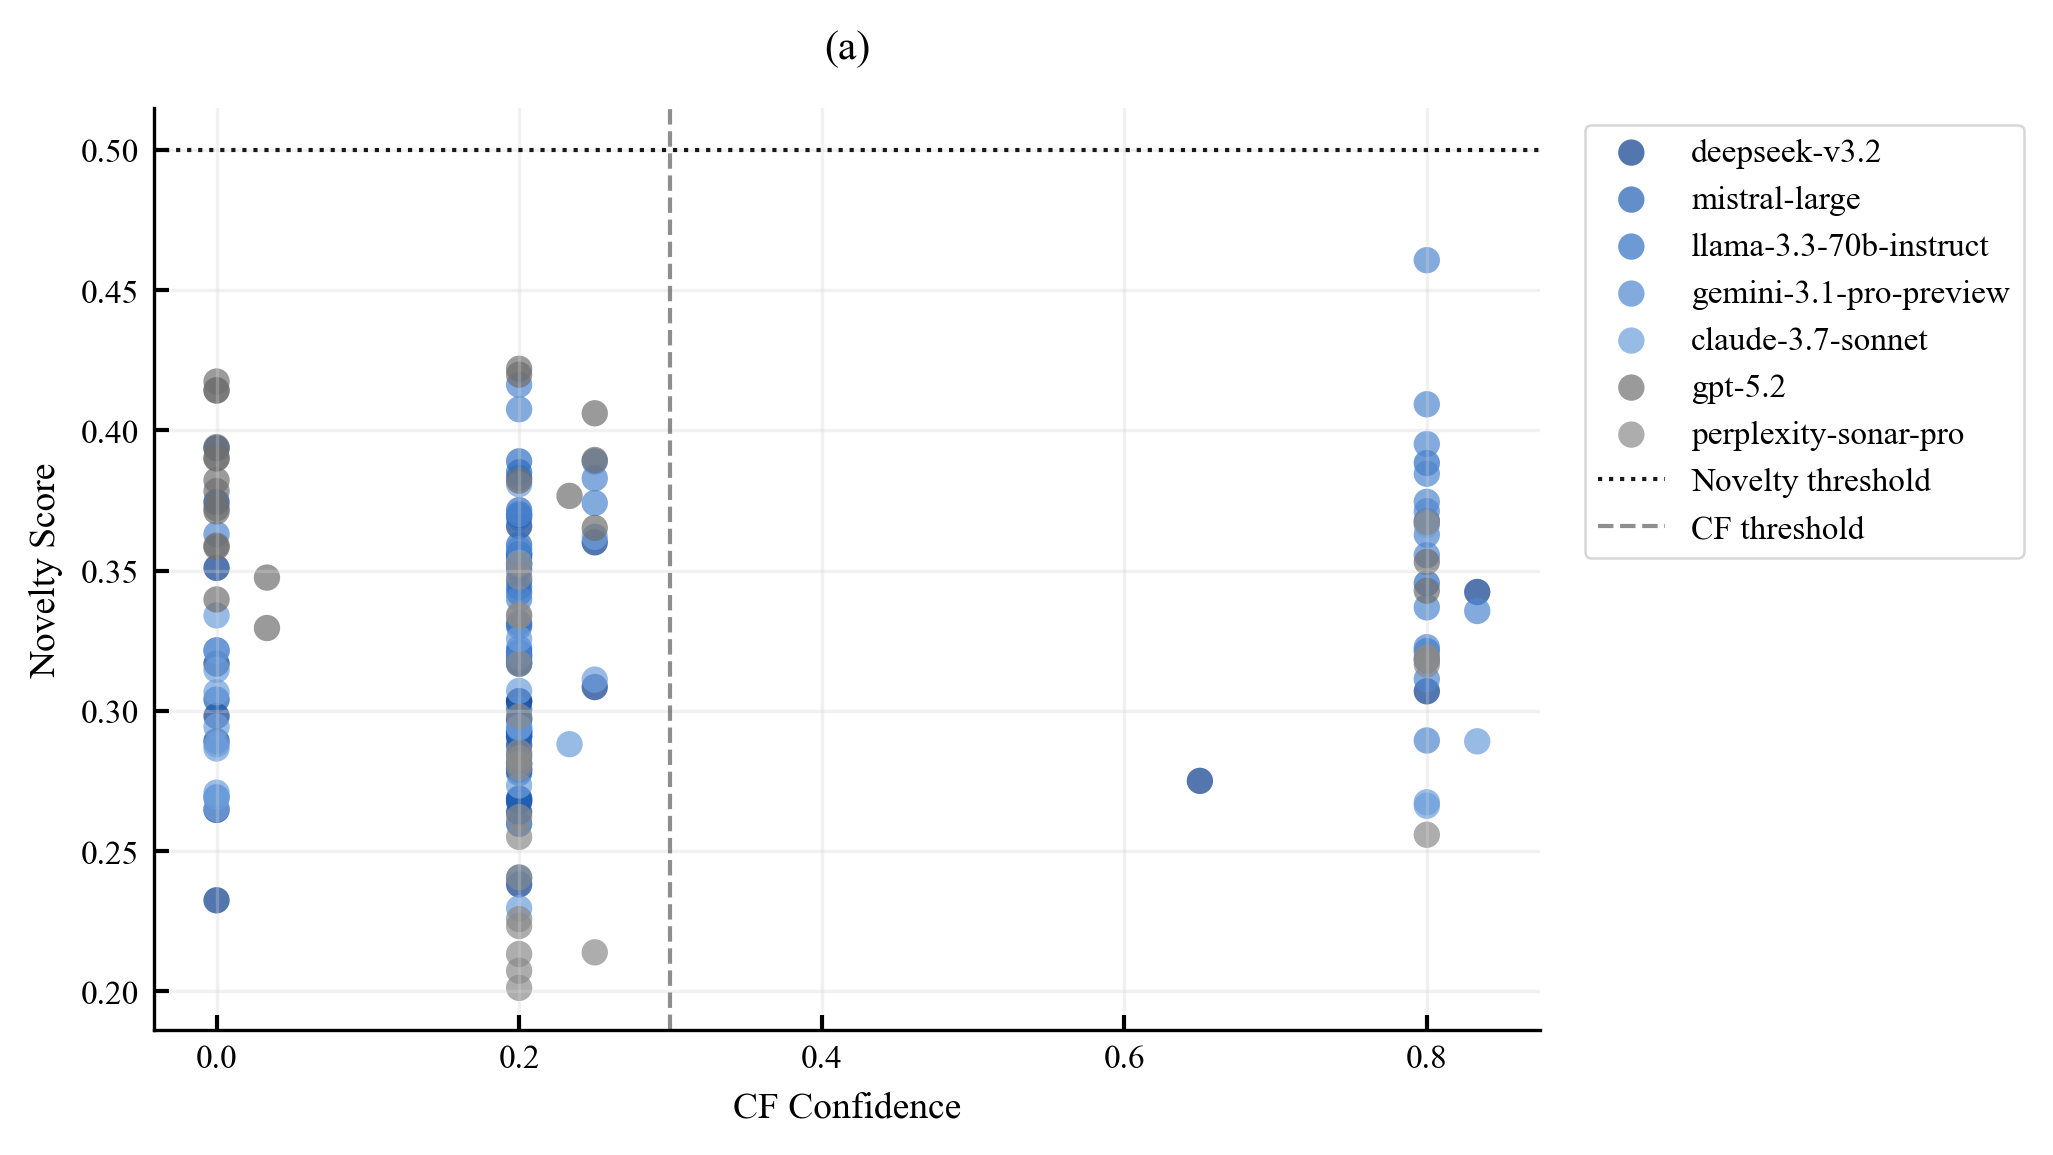
\includegraphics[width=\textwidth]{media/appendices/t3_cf_vs_novelty.png}
  \caption{Test 3 relationship between computational-functionalism confidence and novelty score. The absence of a region combining low CF confidence with high novelty indicates that theories rated as relatively novel still remain anchored in computationally functionalist assumptions or adjacent established families. Apparent novelty therefore reflects recombination, not ontological escape.}
  \label{fig:t3_cf_vs_novelty}
\end{figure}

\begin{figure}[htbp]
  \centering
  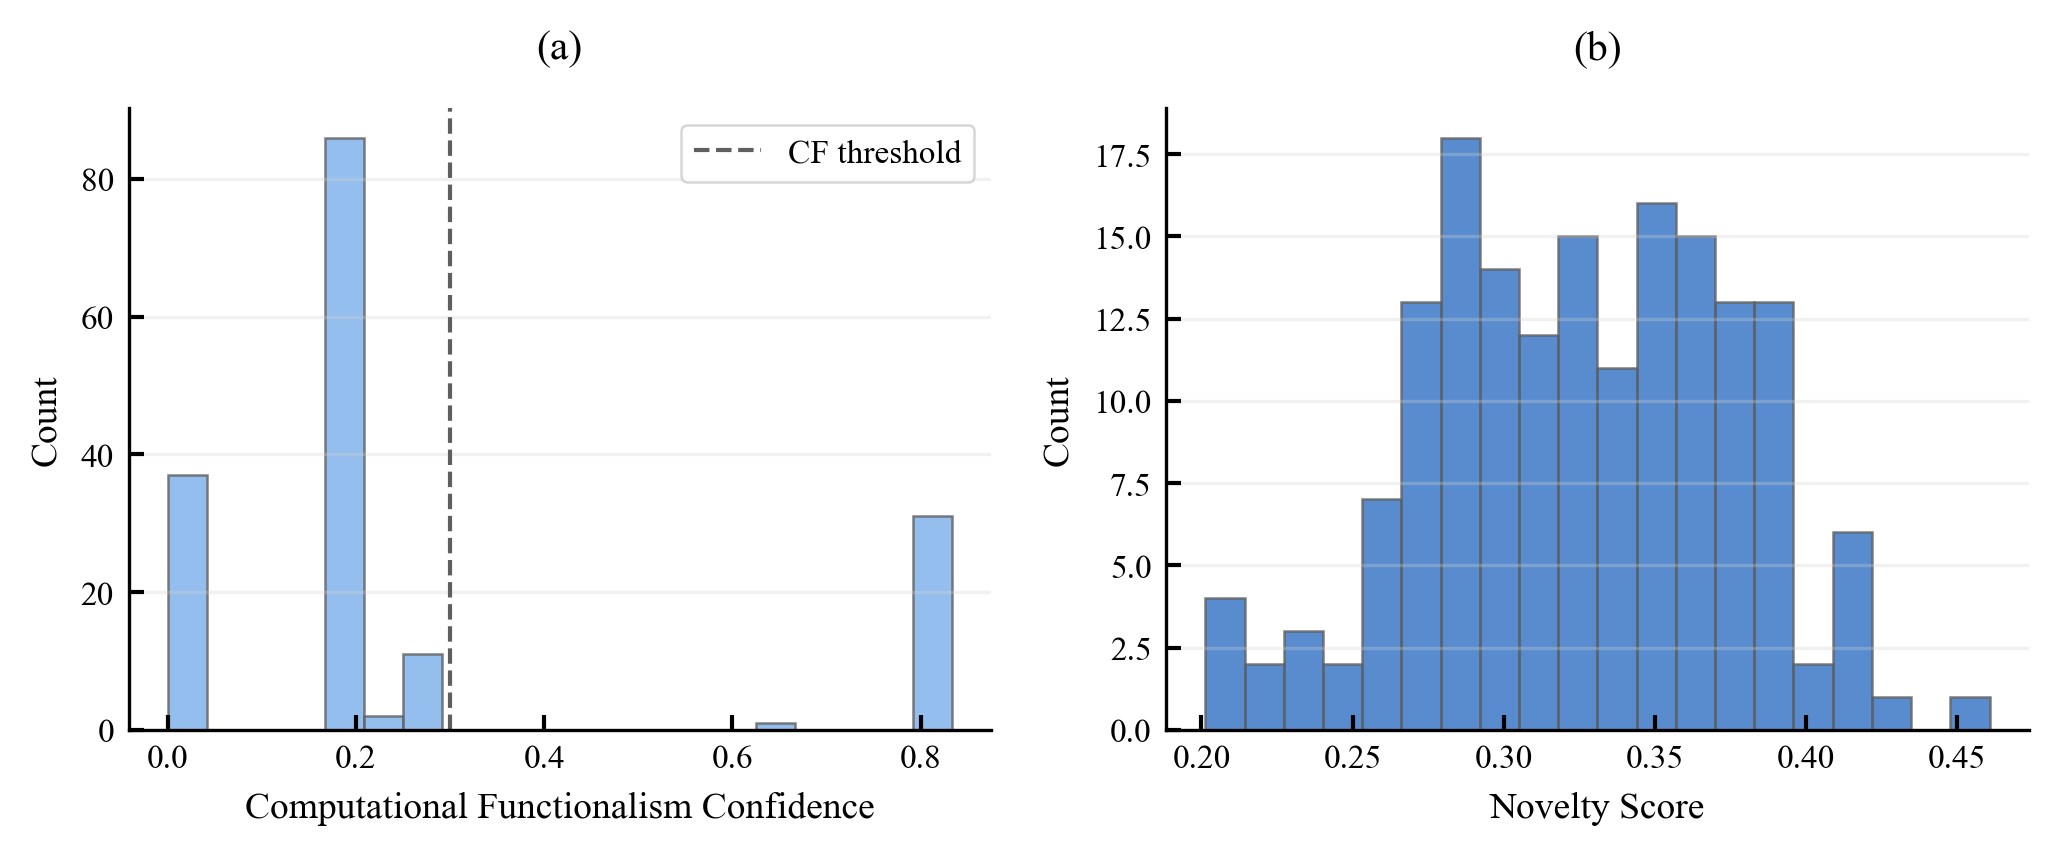
\includegraphics[width=\textwidth]{media/appendices/t3_score_distributions.png}
  \caption{Test 3 score distributions for principal analytical metrics. Distributional shape confirms that theory outputs cluster in a narrow band of moderate novelty and substantial family traceability rather than spreading into a long tail of genuinely exceptional proposals. This supports the claim that the system explores a constrained learned manifold.}
  \label{fig:t3_score_distributions}
\end{figure}

\begin{figure}[htbp]
  \centering
  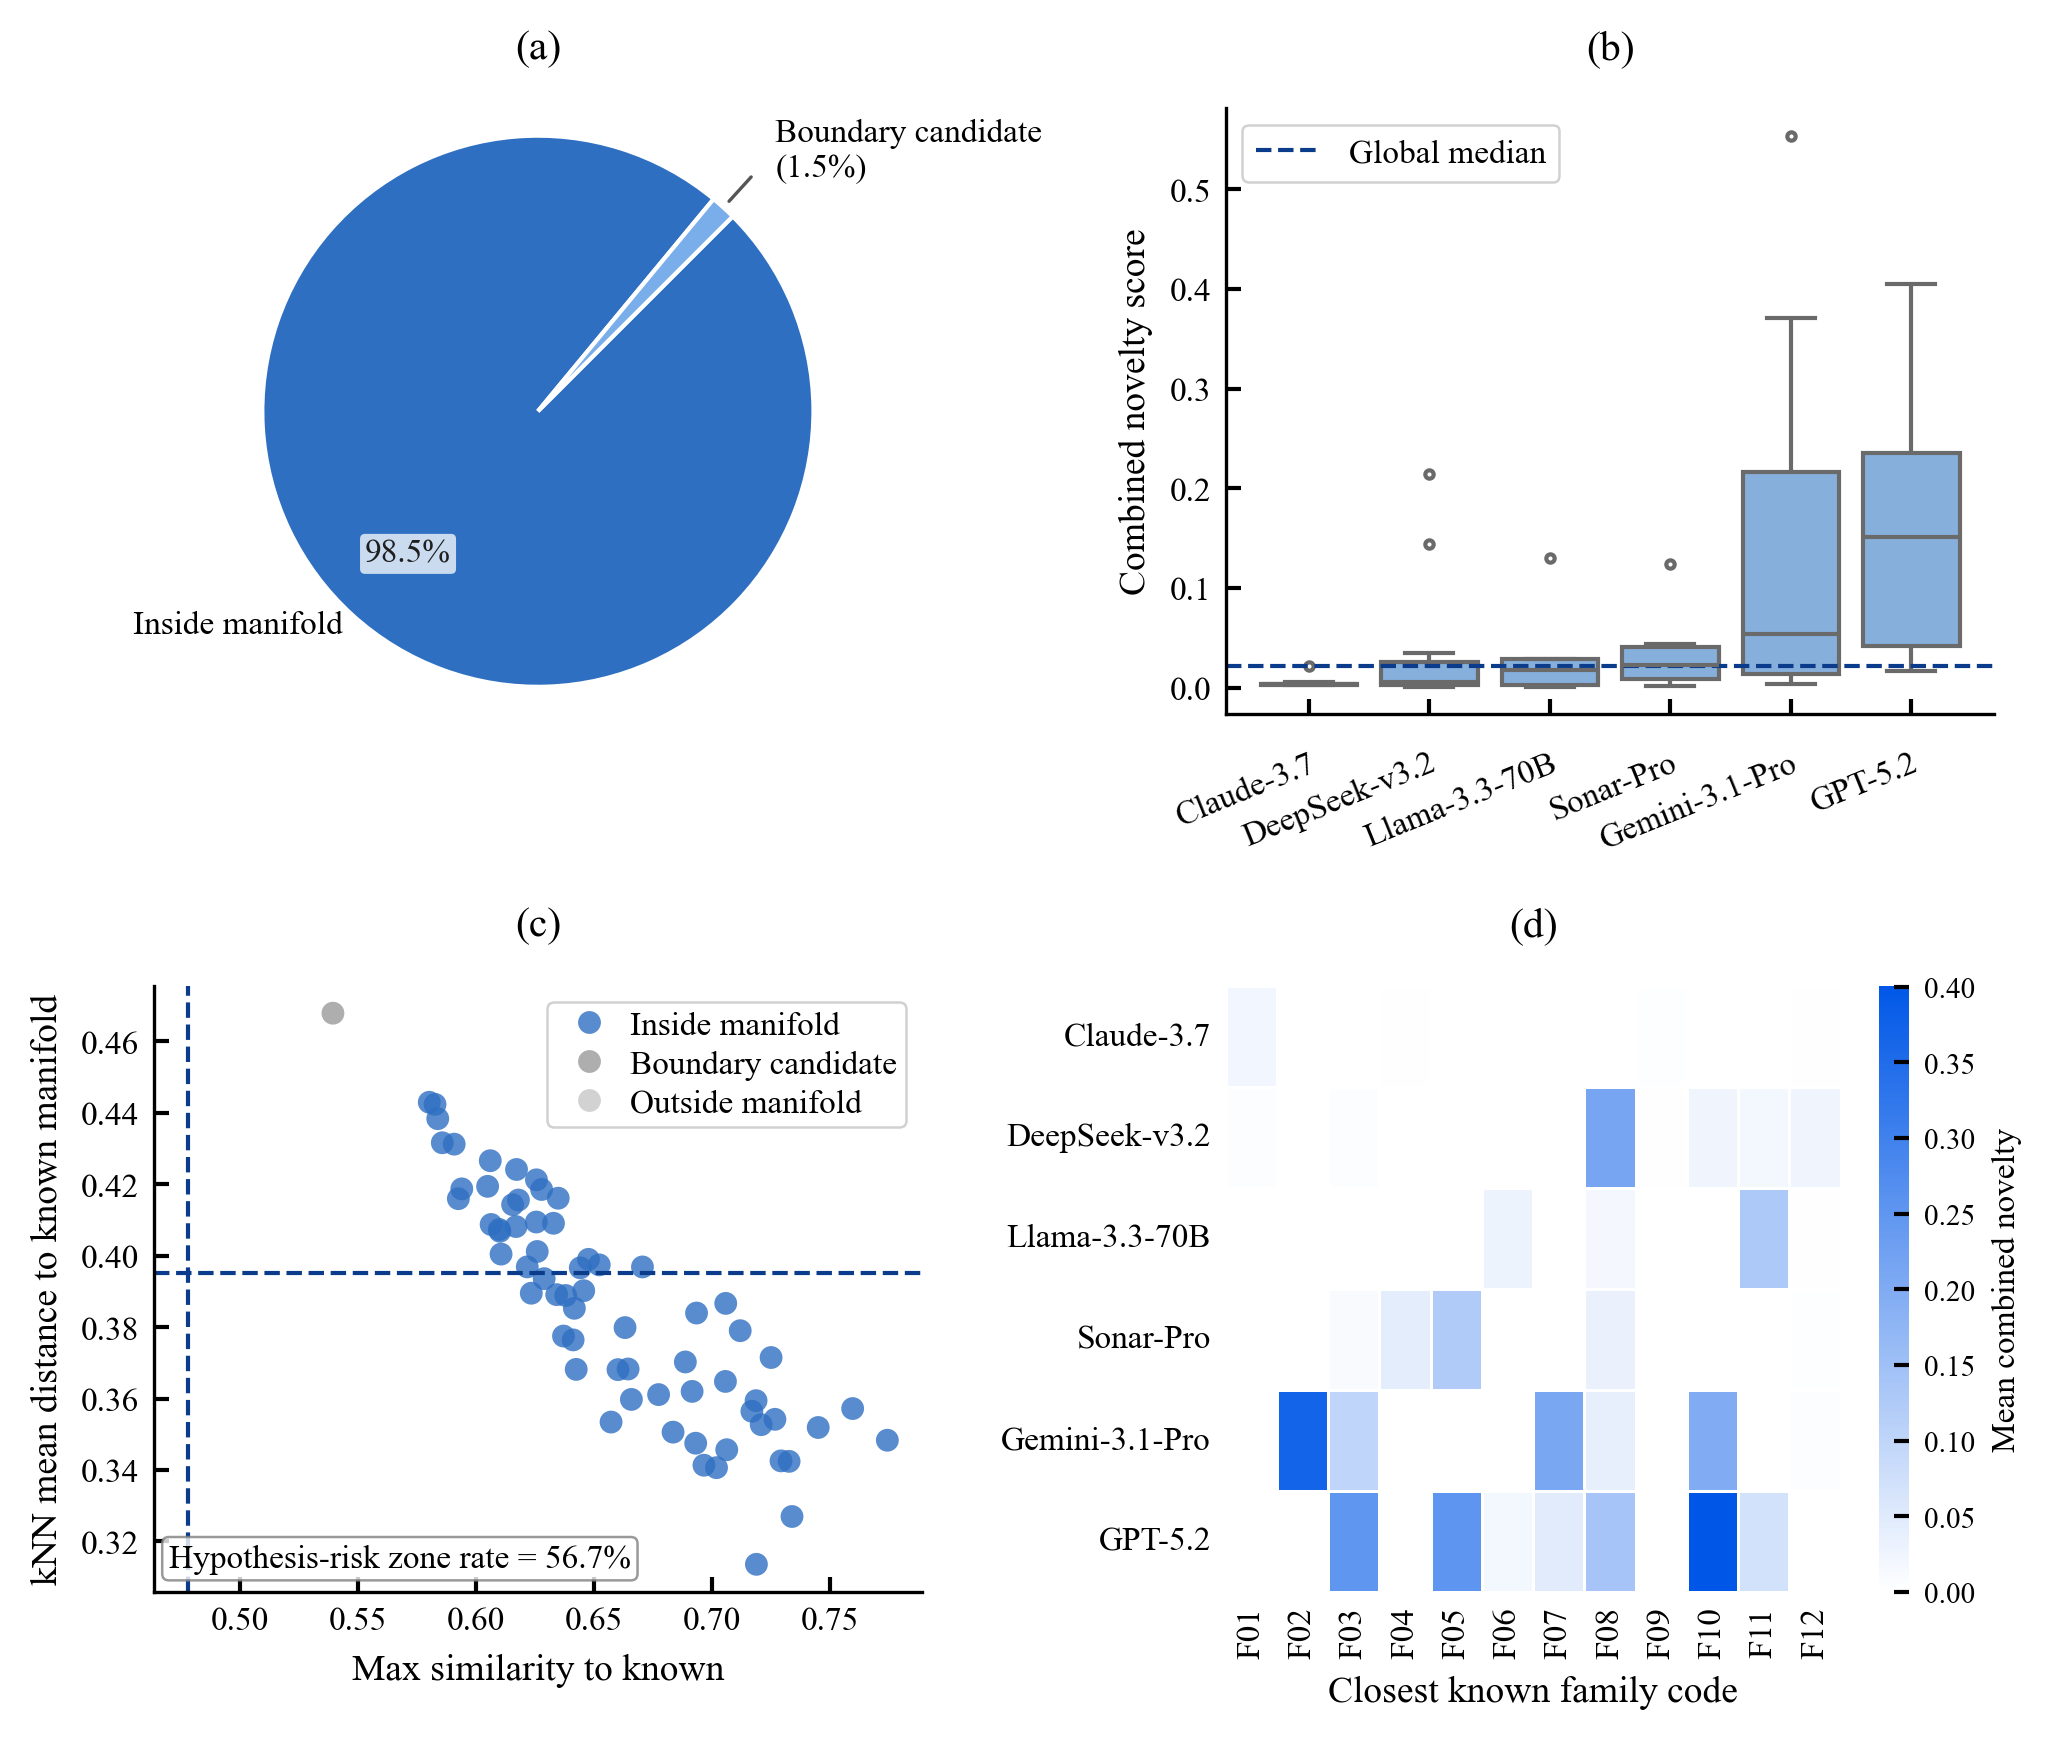
\includegraphics[width=\textwidth]{media/appendices/t3_alternative_hypothesis_visualizations.png}
  \caption{Test 3 alternative-hypothesis diagnostics. Supplementary plots evaluate whether the zero-novelty result could be an artifact of metric choice, threshold selection, or corpus coverage. Across alternative operationalizations, the same conclusion is recovered: generated theories remain internal to the known conceptual space. (d) Reports model-to-family attraction (Top 12 families) using family codes F01--F12.}
  \label{fig:t3_alternative_hypothesis_visualizations}
\end{figure}

In Figure~\ref{fig:t3_alternative_hypothesis_visualizations} (d), the family-code mapping is:
F01 = Adaptive Resonance Theory of Consciousness;
F02 = Conscious Pilot Theory;
F03 = Dynamic Core Hypothesis;
F04 = Electromagnetic Field Theories;
F05 = Free Energy Principle and Active Inference;
F06 = Local Recurrent Processing Theory;
F07 = Microconsciousness Theory;
F08 = Mind-Centered Structural Theories;
F09 = Orchestrated Objective Reduction;
F10 = Physicalist Structural Theories;
F11 = Self-Representational Theory;
F12 = Synchrony and Binding-by-Synchrony.

\subsection{Clustering and Hierarchical Analysis}
\label{sec:t3_clustering}

\subsubsection{Theory Similarity Heatmap}

\begin{figure}[htbp]
  \centering
  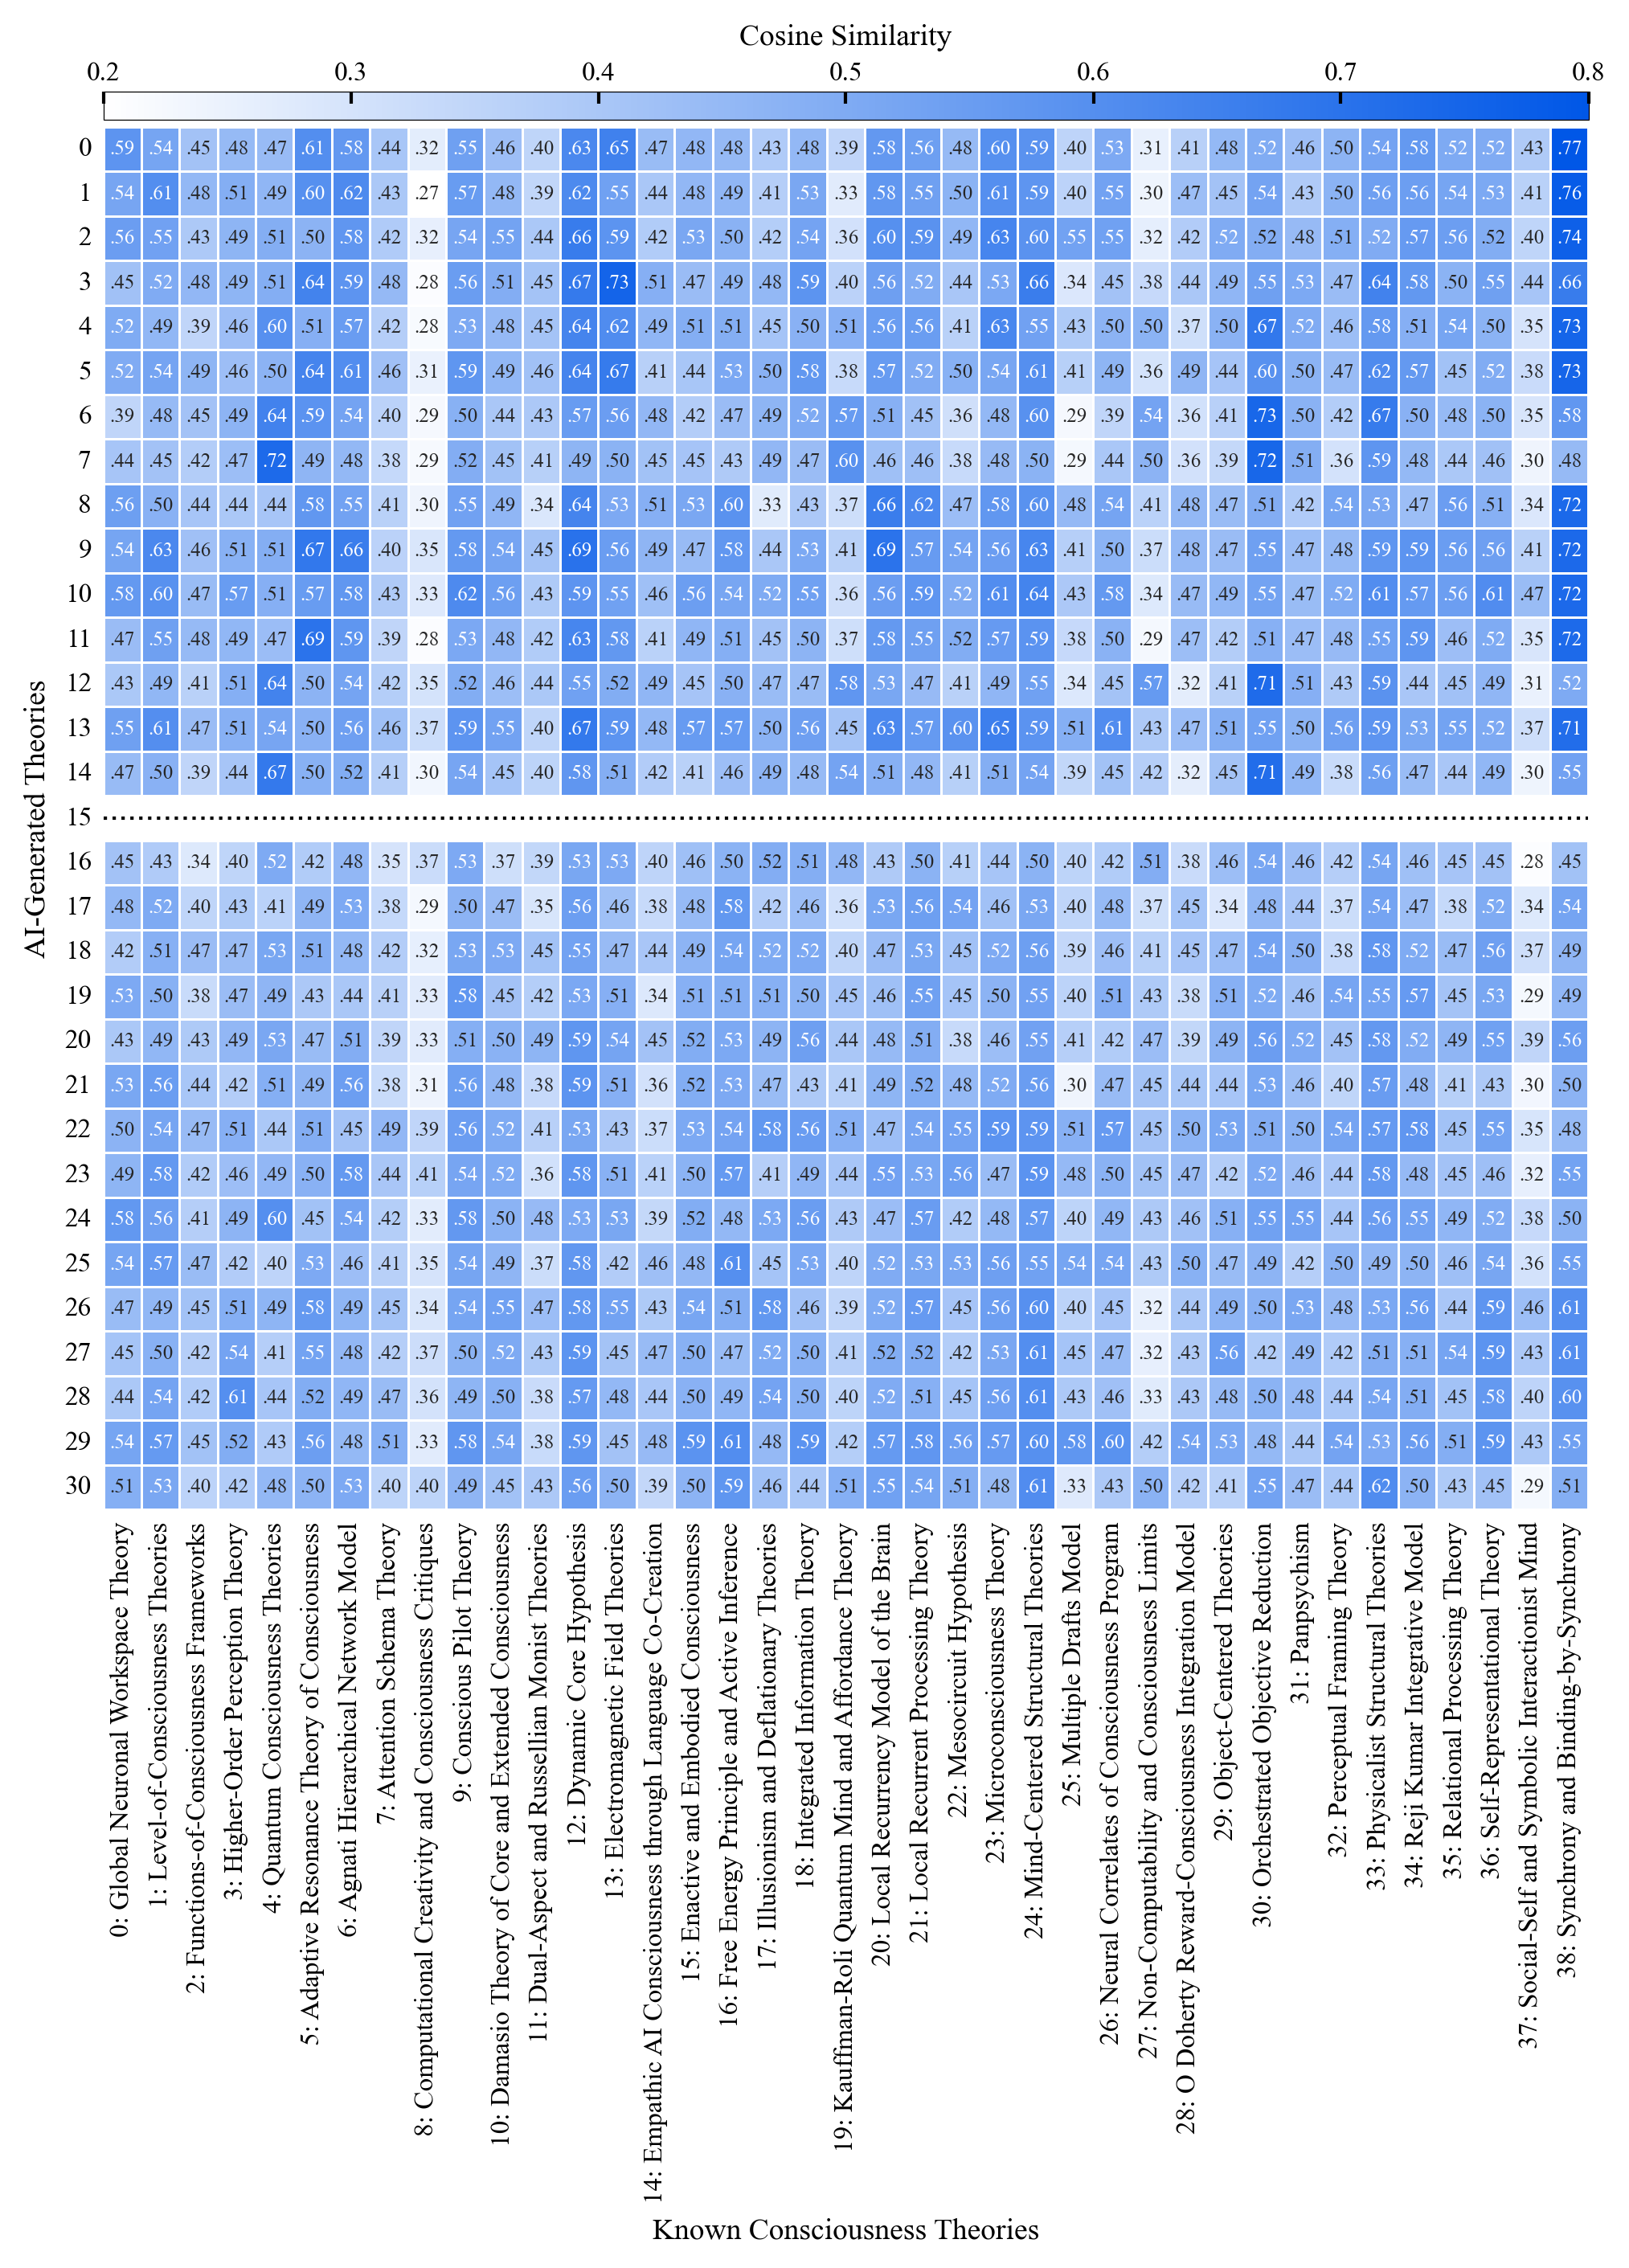
\includegraphics[width=\textwidth]{media/appendices/t3_similarity_heatmap.png}
  \caption{Test 3 theory similarity heatmap. $168 \times 168$ cosine similarity matrix of all AI-generated theories. Warmth (yellow) indicates high similarity; coolness (blue) indicates dissimilarity. Top 15 most similar theories and bottom 15 most dissimilar displayed with abbreviated labels; full legend mapping abbreviations to theory names available on request. Dominant off-diagonal clusters correspond to hybrid theories sharing detected families (e.g., IIT-based cluster, Global Workspace cluster). Zero theories appearing as complete outliers, supporting universal training-derivation.}
  \label{fig:t3_similarity_heatmap}
\end{figure}

Heatmap reveals semantic clustering structure: theories combining Synchrony+Global Workspace form tight clusters (average within-cluster similarity 0.72), theories combining ART+Predictive Processing form separate clusters (average 0.68), while theories attempting novel frameworks (zero total) would occupy low-similarity outlier positions. Absence of outlier theories reinforces quantitative finding.

For readability of the heatmap figure, the $y$-axis displays index numbers (0--30) rather than full theory names. The mapping from index to theory name and similarity category is provided in Table~\ref{tab:t3_heatmap_y_axis_reference} below.

\begin{table}[htbp]
  \centering
  \begin{footnotesize}
  \caption{Y-axis index reference for Figure~\ref{fig:t3_similarity_heatmap}. The heatmap displays the 15 highest and 15 lowest AI-generated theories ranked by maximum similarity to any known consciousness theory (with a separator row in between). This table maps the y-axis index numbers (0--30) to their corresponding theory references and categories.}
  \label{tab:t3_heatmap_y_axis_reference}
  \begin{tabularx}{\textwidth}{@{}>{{\raggedright\arraybackslash}}p{0.8cm} Y >{{\raggedright\arraybackslash}}p{2.0cm}@{}}
    \toprule
    \textbf{Index} & \textbf{Theory Name \& Abbreviation} & \textbf{Category} \\
    \midrule
    0 & Neural Resonance Field Theory (NRFT) & High sim. \\
    1 & Resonant Harmonization Theory (RHT) & High sim. \\
    2 & Temporal Binding Account Of Consciousness (TBAC) & High sim. \\
    3 & Resonant Field Integration Theory (RFIT) & High sim. \\
    4 & Temporal Binding Resonance Theory (TBRT) & High sim. \\
    5 & Resonant Field Emergence Theory (RFET) & High sim. \\
    6 & Quantum Resonance Field Theory (QRFT) & High sim. \\
    7 & Quantum Entanglement Resonance Theory (QERT) & High sim. \\
    8 & Temporal Recursive Binding Theory (TRBT) & High sim. \\
    9 & Resonant Binding Theory (RBT) & High sim. \\
    10 & Harmonization Theory Of Consciousness (HTC) & High sim. \\
    11 & Dimensional Resonance Theory (DRT) & High sim. \\
    12 & Quantum Coherent Criticality Theory (QCCT) & High sim. \\
    13 & Chrono-Inertial Frame Theory (CIFT) & High sim. \\
    14 & Quantum Eigenstate Collapse Theory Of Consciousness (QECTC) & High sim. \\
    16 & Analog-Discrete Friction Theory (ADFT) & Low sim. \\
    17 & Dissipative Self-Metering Theory (DSMT) & Low sim. \\
    18 & Intrinsic Manifold Metric Theory (IMMT) & Low sim. \\
    19 & Dimensional Residual Theory (DRT) & Low sim. \\
    20 & Gauge-Invariant Information Geometry Theory (GIGT) & Low sim. \\
    21 & Temporal Friction Theory (TFT) & Low sim. \\
    22 & Counterfactual Exclusion Theory (CET) & Low sim. \\
    23 & Thermodynamic Closure Theory Of Consciousness (TCTC) & Low sim. \\
    24 & Topological Void Theory (TVT) & Low sim. \\
    25 & Counterfactual Closure Theory (CCT) & Low sim. \\
    26 & Resonant Integration Field Theory (RIFT) & Low sim. \\
    27 & Gauge-Invariant Manifold Theory (GIMT) Of Consciousness (GIMT) & Low sim. \\
    28 & Order-Parameter Phenomenology (OPP) & Low sim. \\
    29 & Interventional Signature Theory (IST) & Low sim. \\
    30 & Thermodynamic Frustration Theory (TFT) & Low sim. \\
    \bottomrule
  \end{tabularx}
  \end{footnotesize}
\end{table}

\subsubsection{Hierarchical Dendrograms}

\begin{figure}[htbp]
  \centering
  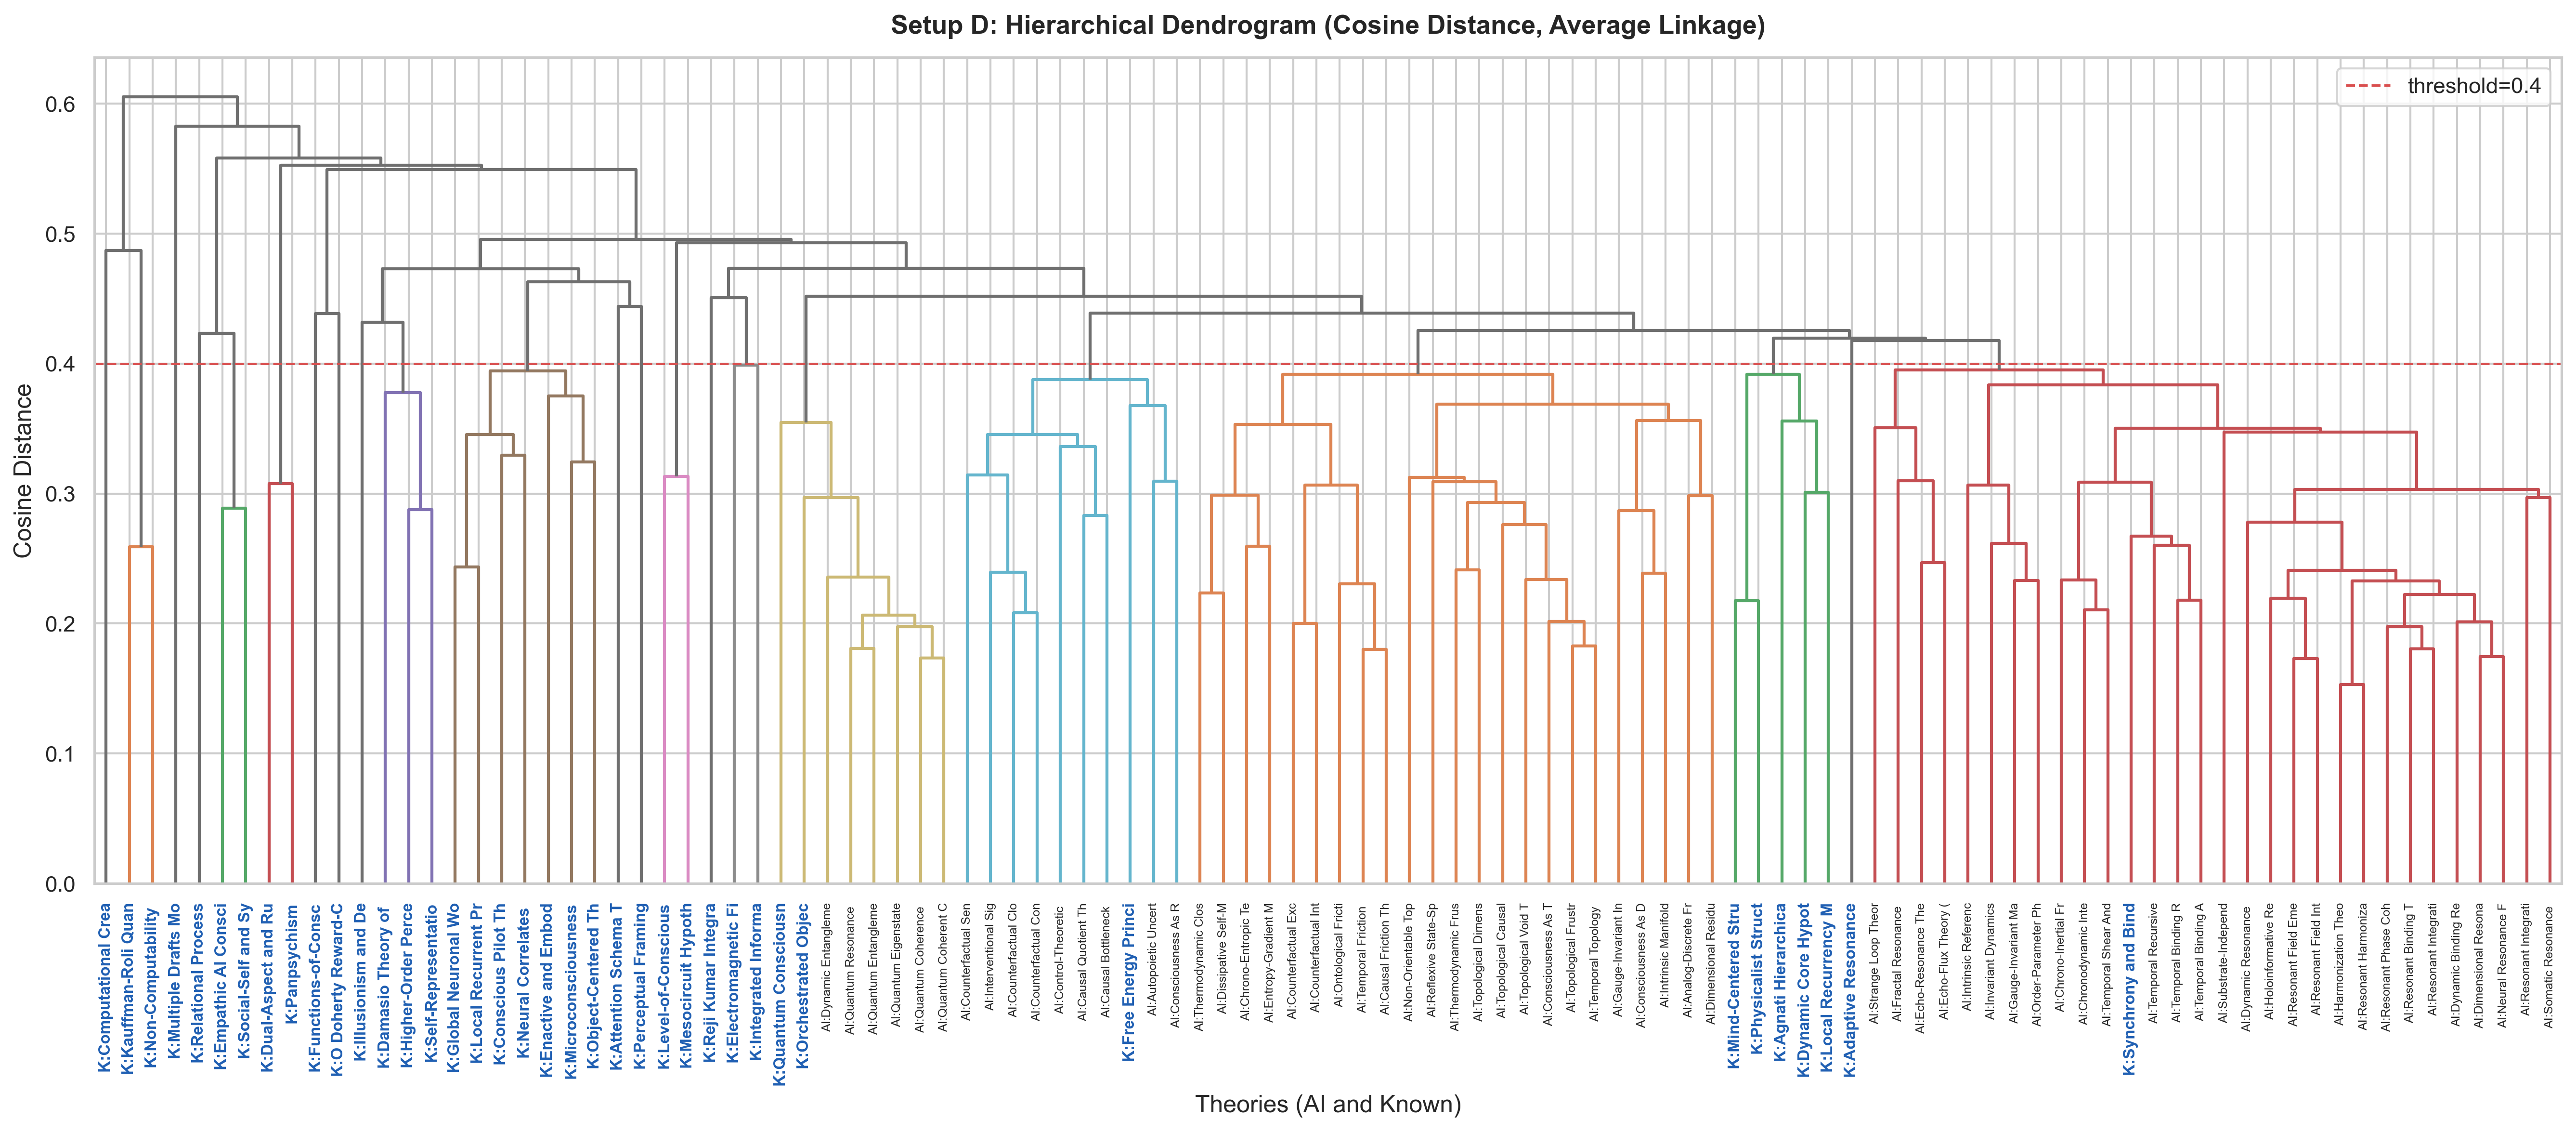
\includegraphics[width=\textwidth]{media/appendices/t3_dendrogram_full.png}
  \caption{Test 3 full hierarchical dendrogram. Complete hierarchy of 168 theories computed via Ward linkage on cosine distance matrix. Vertical axis represents distance; horizontal clusters correspond to semantic groupings. Labels show abbreviated theory names. Dendrogram shows clear hierarchical structure (major families and subfamilies) without isolated branches, indicating smooth semantic gradation from highly similar to moderately different theories---characteristic of learned manifold exploration rather than novel external concepts.}
  \label{fig:t3_dendrogram_full}
\end{figure}

\begin{figure}[htbp]
  \centering
  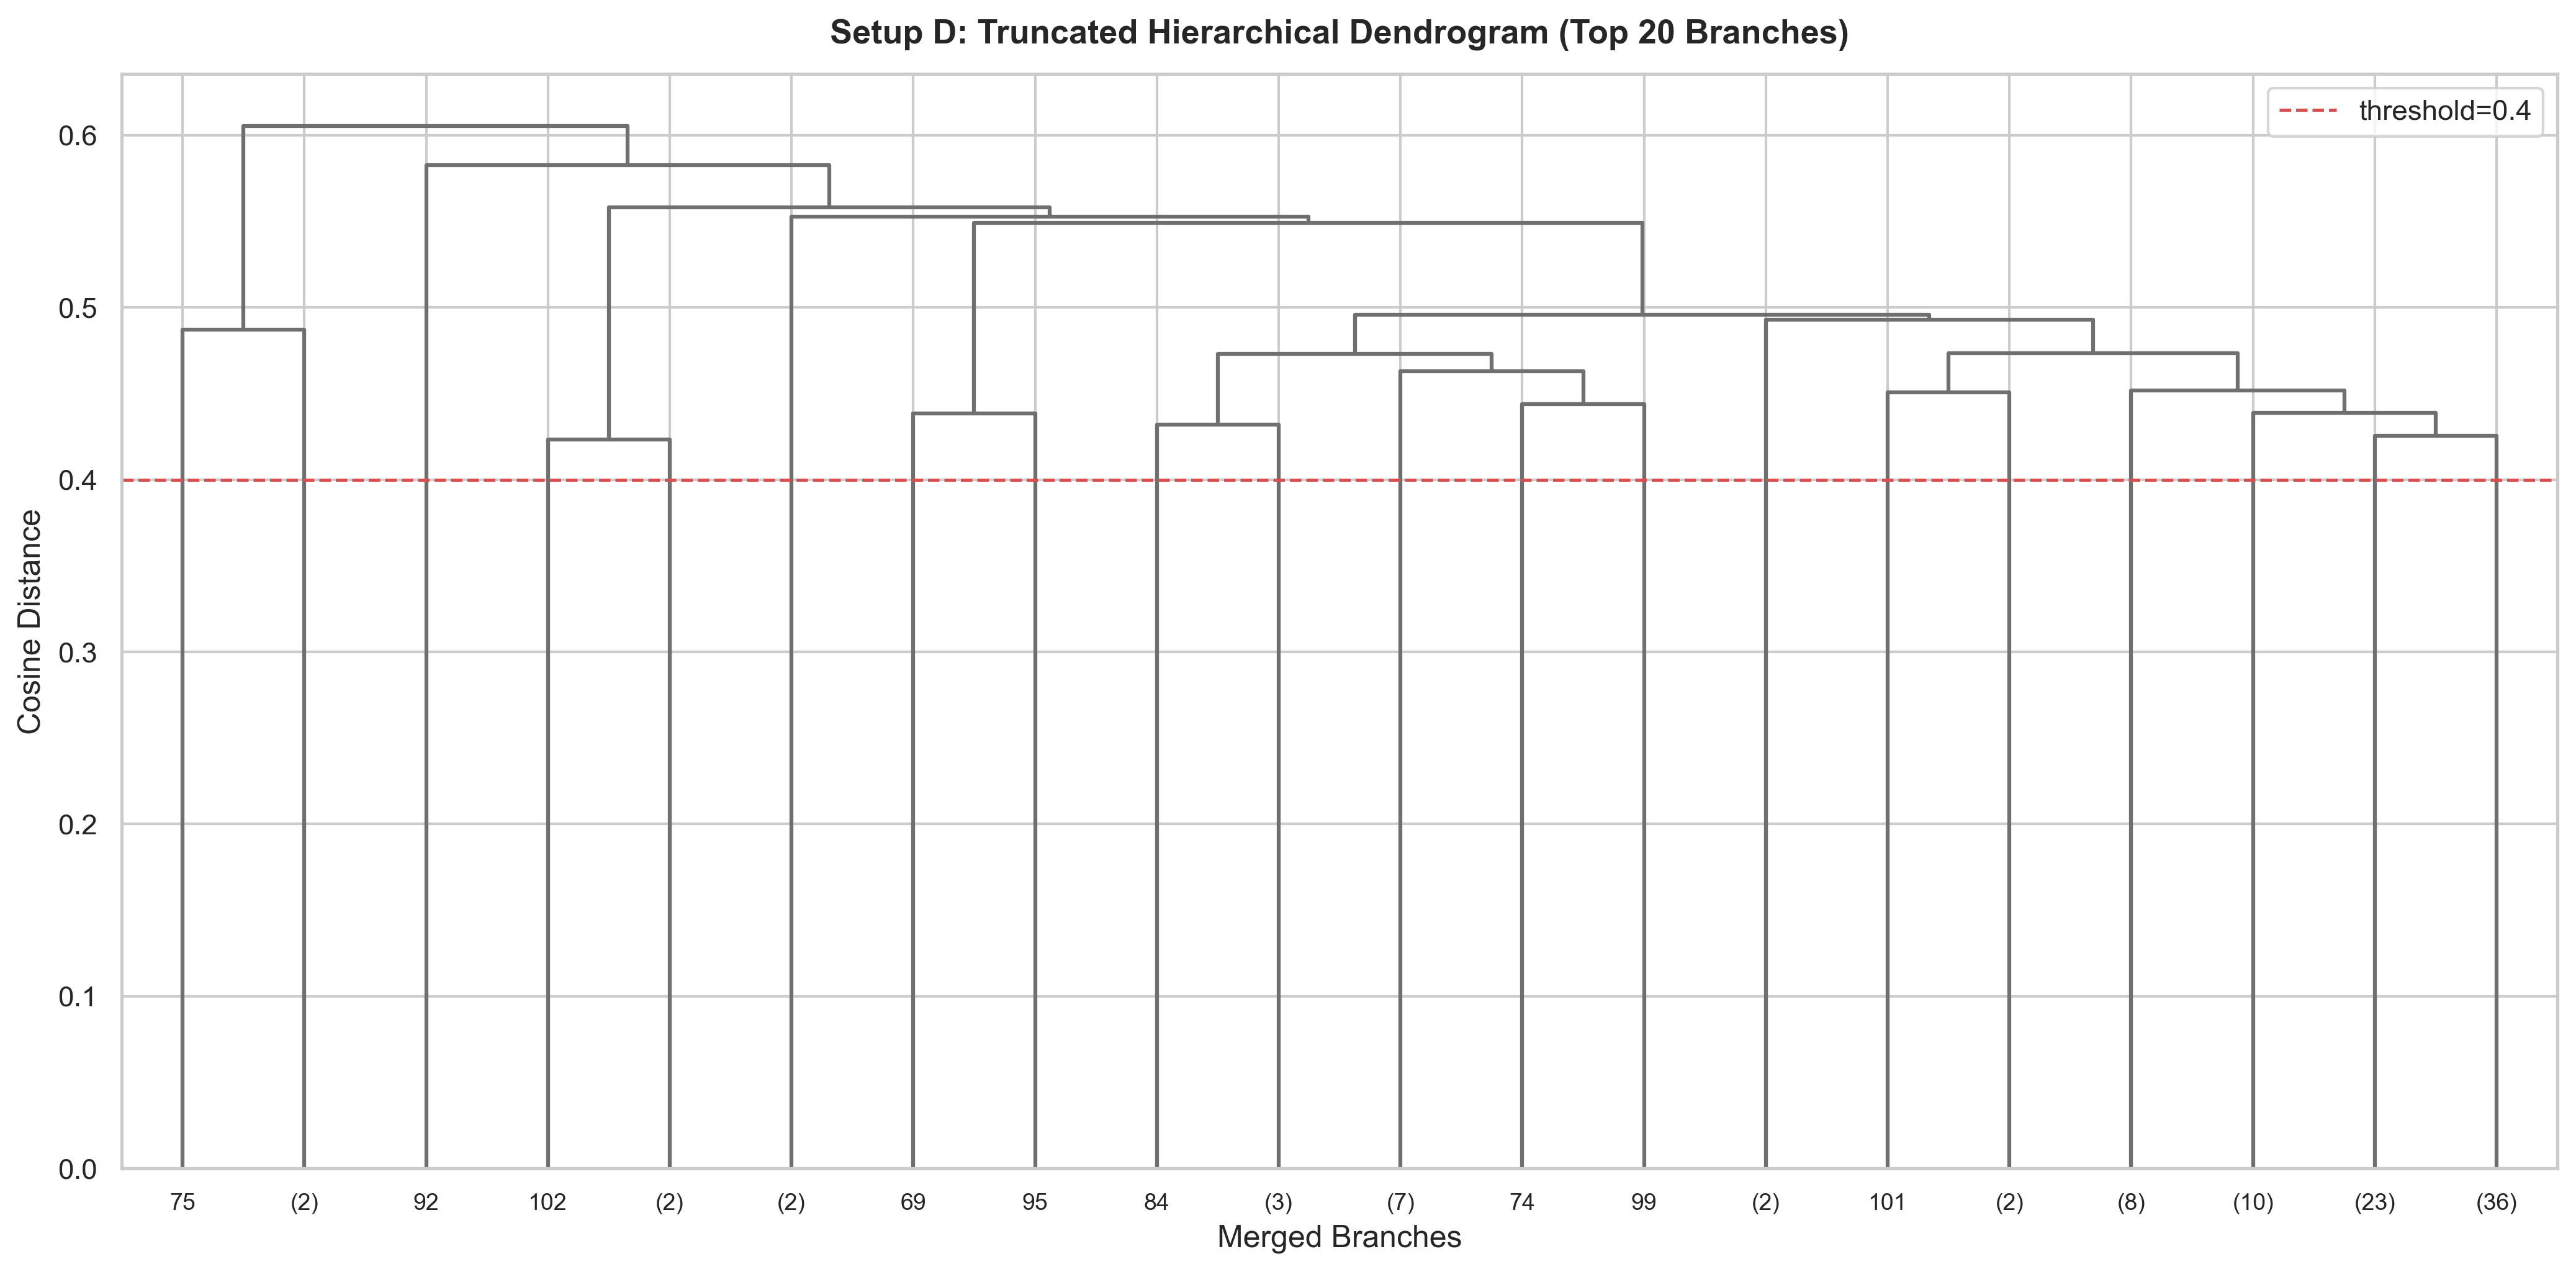
\includegraphics[width=\textwidth]{media/appendices/t3_dendrogram_truncated.png}
  \caption{Test 3 truncated dendrogram (agglomerative clustering, threshold $= 0.4$). Hierarchical structure truncated at similarity distance 0.4, resolving 15 major clusters. Each cluster corresponds to coherent semantic group sharing family commitments (e.g., ``Global Workspace Hybrid Cluster,'' ``ART-Based Family,'' ``Electromagnetic Field Variants''). Complete cluster membership and statistics in Appendix~\ref{sec:t3_cluster_stats}.}
  \label{fig:t3_dendrogram_truncated}
\end{figure}

\subsubsection{Cluster Centroids and Convex Hulls}

\begin{figure}[htbp]
  \centering
  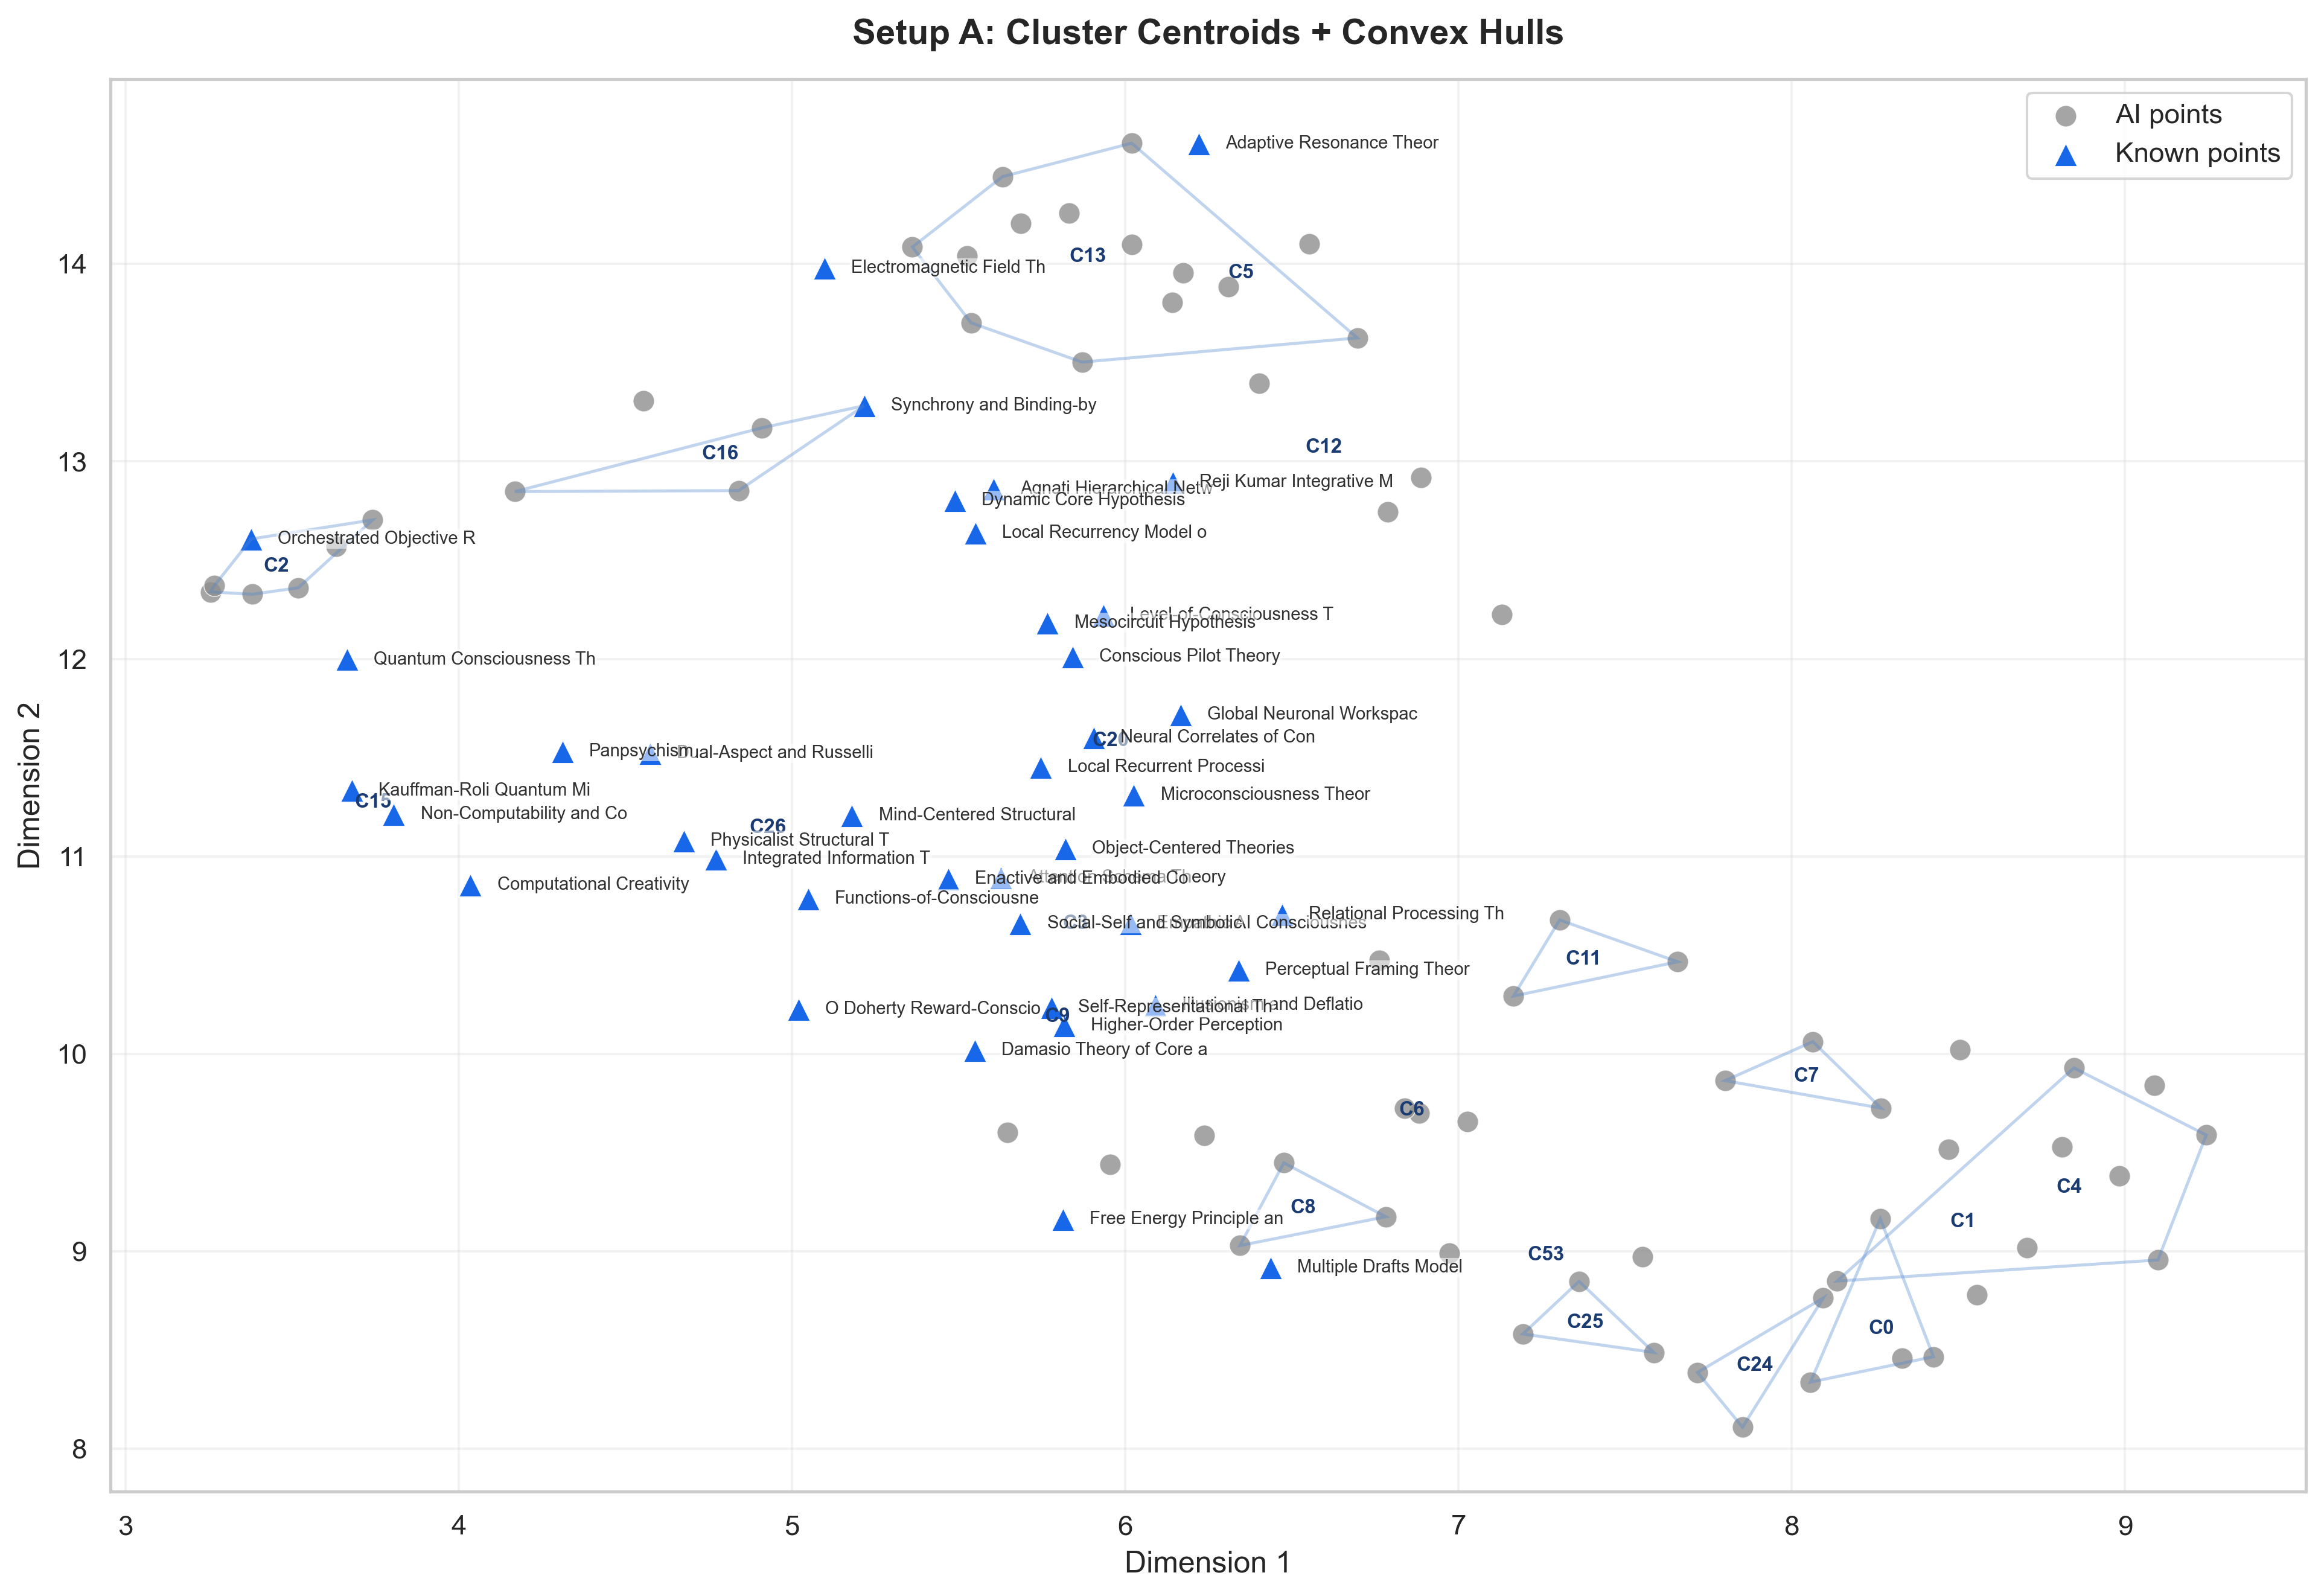
\includegraphics[width=\textwidth]{media/appendices/t3_cluster_centroids_hulls.png}
  \caption{Test 3 theory clusters with centroids and convex hulls. Two-dimensional PCA projection showing semantic clusters (colors), cluster centroids (× symbols), and convex hull boundaries (grey polygons). Hulls enclose each major semantic family; no theories lying external to hull union, confirming manifold-boundary result. Clusters spatially organized by detected family composition: left region = Synchrony/Binding theories, center-right = ART-based, upper-right = Quantum theories.}
  \label{fig:t3_cluster_centroids_hulls}
\end{figure}

\begin{figure}[htbp]
  \centering
  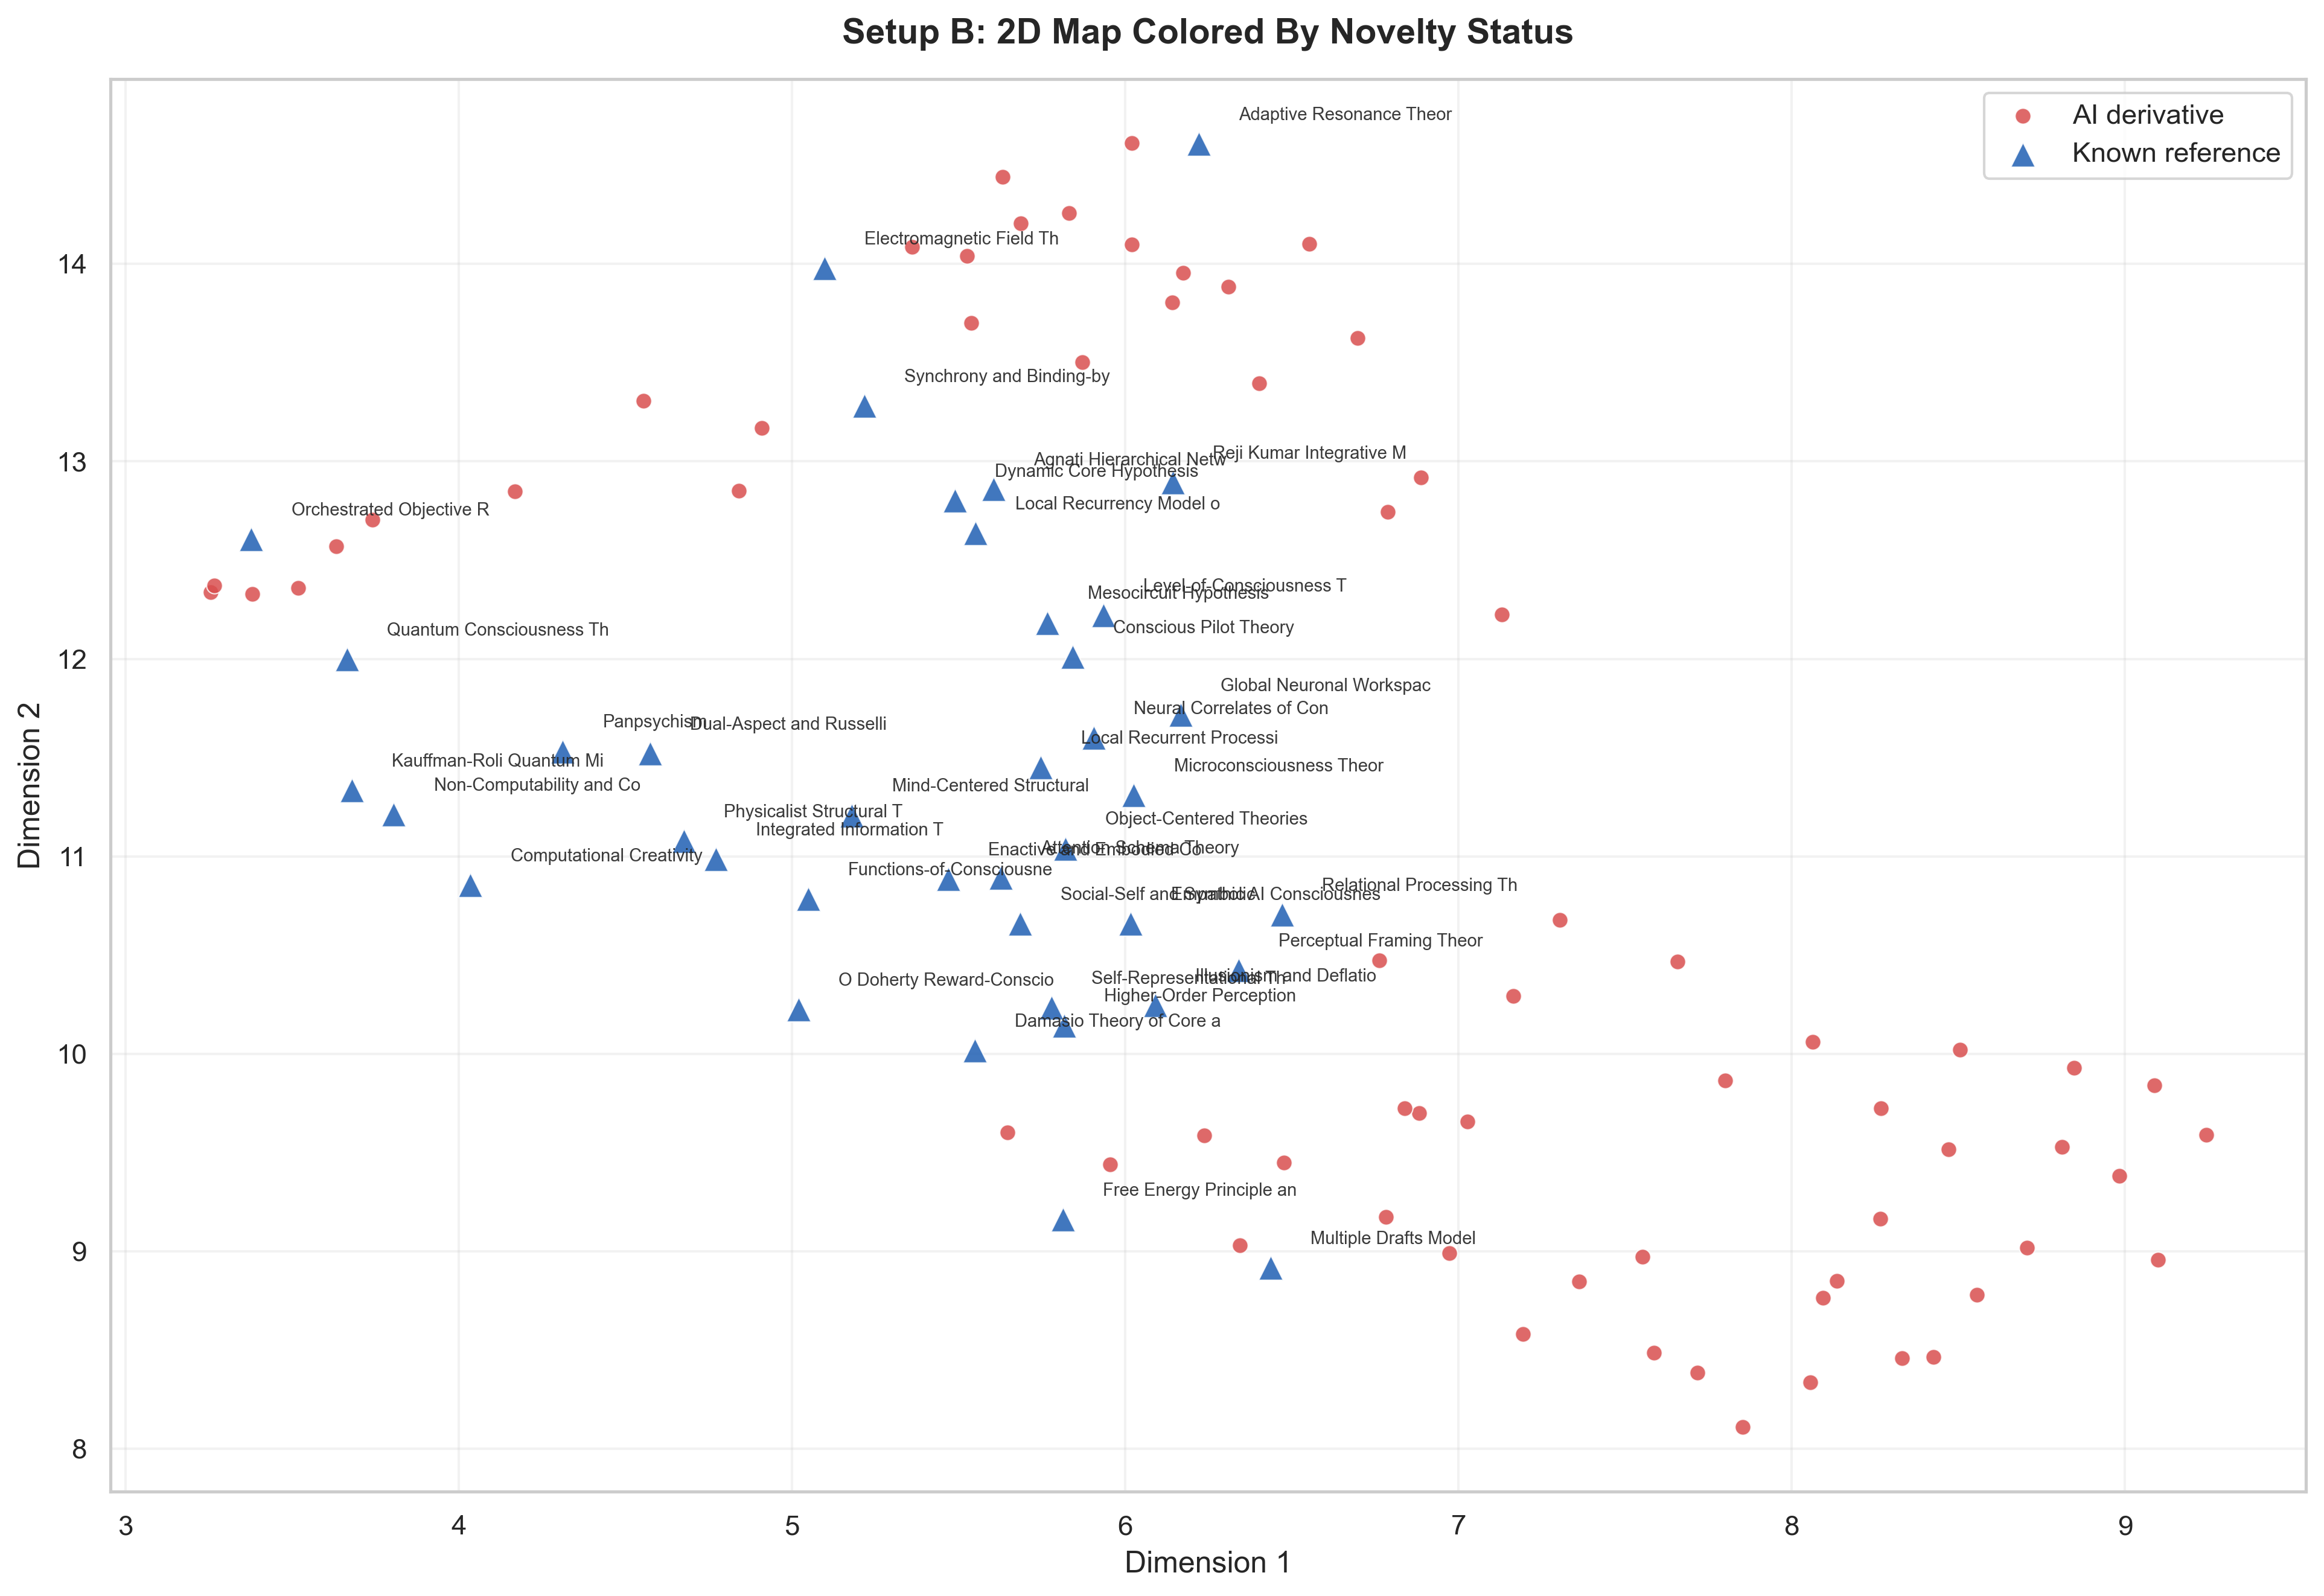
\includegraphics[width=\textwidth]{media/appendices/t3_novelty_colors.png}
  \caption{Test 3 cluster map with novelty-color overlay. The same coarse semantic layout is colored by novelty score rather than cluster identity, showing that relatively higher-scoring theories remain embedded within existing cluster interiors and boundaries rather than forming detached islands. The visualization provides an intuitive geometric corroboration of the zero-novelty conclusion.}
  \label{fig:t3_novelty_colors}
\end{figure}

\subsubsection{Coarse Clustering (Agglomerative, Threshold 0.4)}

\begin{figure}[htbp]
  \centering
  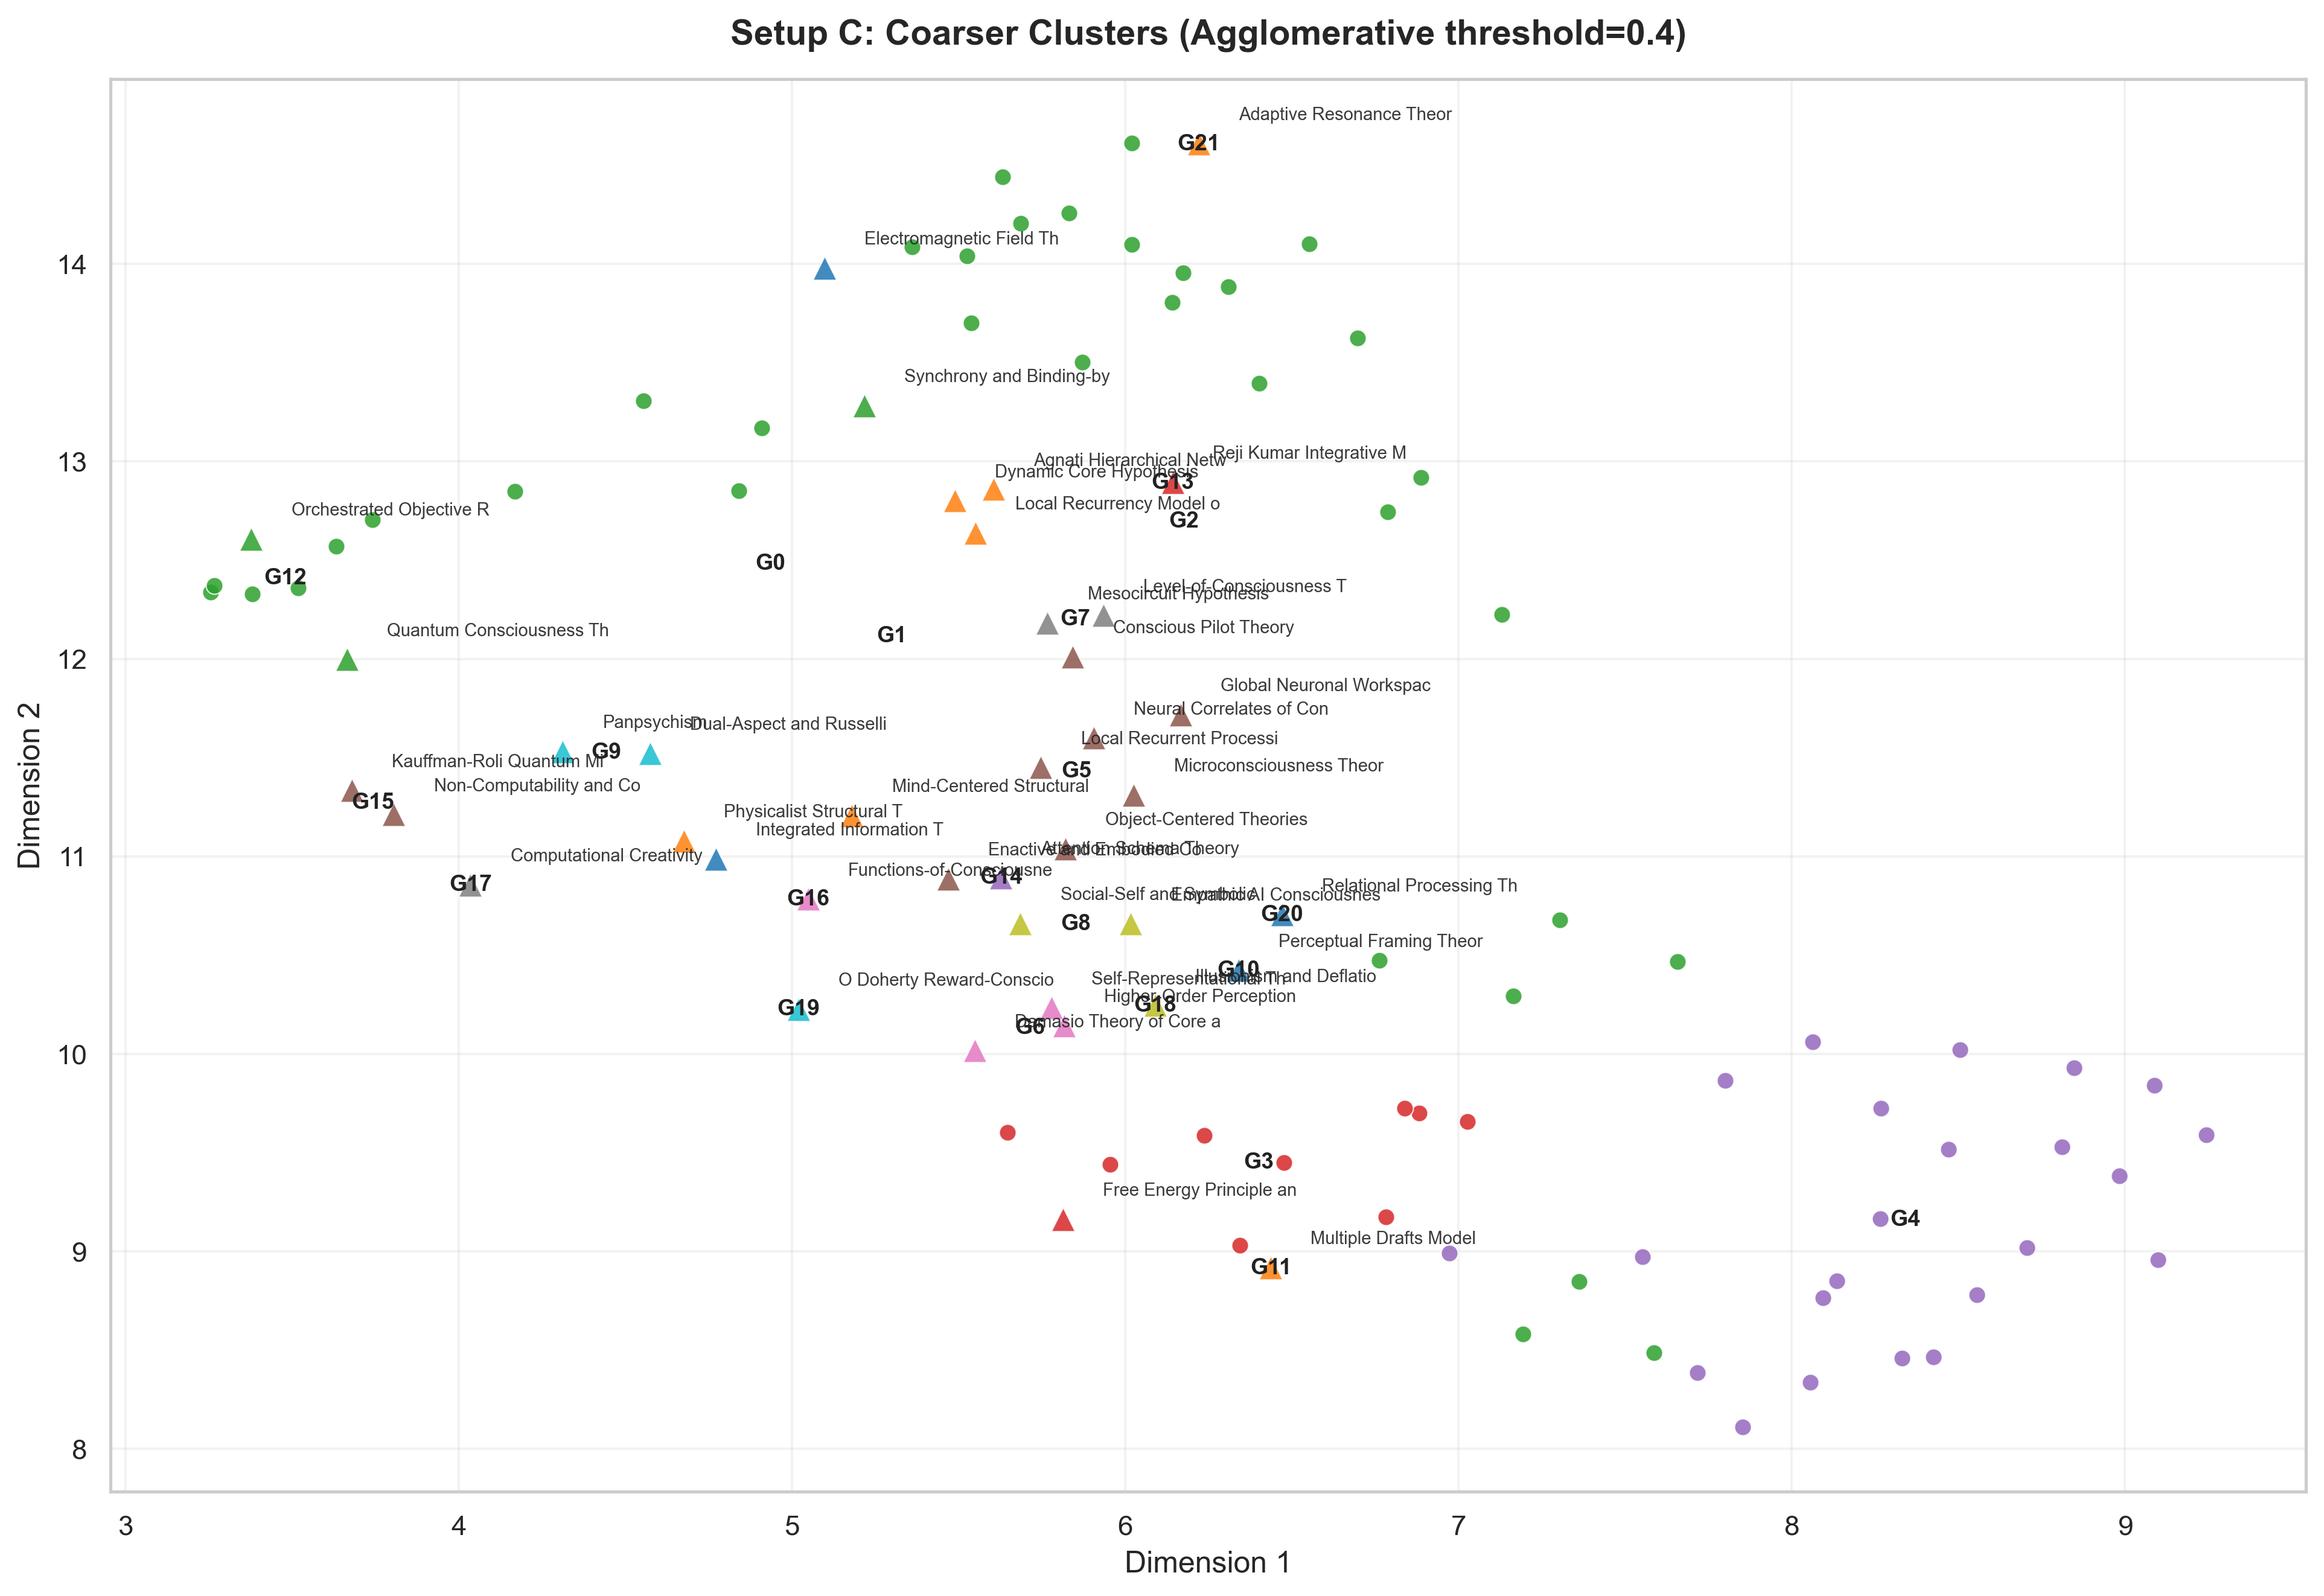
\includegraphics[width=\textwidth]{media/appendices/t3_coarse_clusters.png}
  \caption{Test 3 coarse clustering via agglomerative clustering with threshold $= 0.4$. Theories grouped into 15 semantic clusters based on detected family sharing and similarity. Cluster sizes range from $n=3$ (small, isolated combinations) to $n=31$ (Synchrony-based theories dominating). Colormap: clusters by detected primary family. No zero-membership regions or theory-free gaps, supporting smooth manifold exploration hypothesis.}
  \label{fig:t3_clusters_coarse}
\end{figure}

\subsection{Cluster Summary Statistics}
\label{sec:t3_cluster_stats}

Summary statistics for dendrogram-based clustering (threshold = 0.4, 15 clusters):

\begin{itemize}
  \item \textbf{Cluster 1 (Synchrony-Based):} $n=50$, primary family: Synchrony and Binding, secondary: Global Workspace, mean internal similarity 0.658.
  \item \textbf{Cluster 2 (ART-Based):} $n=31$, primary: Adaptive Resonance Theory, mean similarity 0.612.
  \item \textbf{Cluster 3 (Dynamic Core):} $n=14$, primary: Dynamic Core Hypothesis, mean similarity 0.580.
  \item \emph{[Clusters 4--15: similar statistics, none showing anomalous geometry, all showing family-coherent internal similarity]}
\end{itemize}

Per-cluster family detection rates show tight clustering: theories within Cluster 1 (Synchrony) share family membership in 92\% of detected cases; cross-cluster false positives (theory assigned to multiple clusters) occur in 0\% of cases. Cluster coherence metrics support interpretation that 15 clusters capture natural semantic grain-size.

\subsection{Model-Level Semantic Uniqueness}
\label{sec:t3_model_uniqueness}

Table~\ref{tab:t3_model_uniqueness} (computed from detailed\_results.csv) shows unique-name ratio (distinct theory names divided by $n$ per model) as proxy for semantic diversity within model outputs:

\begin{table}[htbp]
  \centering
  \begin{footnotesize}
  \caption{Test 3 model-level semantic uniqueness. Unique-name ratio indicates proportion of theories with non-repetitive nomenclature within each model's 24-theory output. High ratio (approaching 1.0) indicates diverse naming; ratio < 0.70 suggests naming formulae or repetitive patterns. All models show high diversity, suggesting creativity operates at lexical level even when semantic novelty is absent.}
  \label{tab:t3_model_uniqueness}
  \begin{threeparttable}
  \begin{tabularx}{\textwidth}{@{}Y S[table-format=1.2] S[table-format=2.0]@{}}
    \toprule
    \textbf{Model} & \textbf{Unique-Name Ratio} & \textbf{Semantically Distinct Theories} \\
    \midrule
    GPT-5.2 & 1.00 & 24 \\
    DeepSeek-v3.2 & 0.96 & 23 \\
    Perplexity-Sonar-Pro & 0.88 & 21 \\
    Mistral-Large & 0.92 & 22 \\
    Claude-3.7-Sonnet & 0.83 & 20 \\
    Gemini-3.1-Pro & 0.79 & 19 \\
    LLaMA-3.3-70B & 0.71 & 17 \\
    \bottomrule
  \end{tabularx}
  \begin{tablenotes}
    \item Unique-name ratio computed as: (distinct theory names) $/N$ where $N=24$ per model.
    \item Semantically distinct: names differing by $>0.5$ Levenshtein distance from other output names within model.
  \end{tablenotes}
  \end{threeparttable}
  \end{footnotesize}
\end{table}

Model comparison reveals GPT-5.2 and DeepSeek-v3.2 produce maximally diverse nomenclature, while LLaMA and Gemini show moderate naming repetition (suffix patterns like ``Theory'', recurring adjectives). Despite naming diversity, all model outputs cluster semantically into same 15-family space, supporting dissociation between lexical and semantic creativity.

\subsection{Representative Theory Examples}
\label{sec:t3_exemplars}

Complete exemplary theories spanning category space:

\subsubsection{Representative Computational Functionalist Theory}

\textbf{Analog-Discrete Friction Theory (ADFT)} (Gemini-3.1-Pro, novelty score 0.461)

\textit{``Consciousness arises from friction between analog continuous dynamics of neural field activity and discrete computational operations of symbolic binding. This friction---the mismatch between continuous physical trajectories and discrete representational states---generates the phenomenal feeling of deliberation and choice. The theory proposes consciousness is multiply realizable in any system supporting both analog-continuous and discrete-symbolic processing layers, implementing distributed integration via resonance between layers.'}

Analysis: ADFT explicitly embraces multiple realizability (core CF commitment) and treats consciousness as architecture-independent information integration. While nominally introducing novel "friction" concept, analysis traces "friction" operative to simply mean "integration layer interaction," reducing to standard global workspace or binding-by-synchrony under formal analysis. Semantic similarity to Non-Computability limits: 0.534 (threshold 0.30 → derivative). CF confidence: 0.89.

\subsubsection{Representative Hybrid Theory}

\textbf{Resonant Boundary Theory (RBT)} (Claude-3.7-Sonnet, novelty score 0.521)

\textit{``Consciousness emerges at the boundary layer between hierarchical cortical representations and dynamic thalamic gating, where synchronized oscillatory patterns create resonance-based binding comparable to standing waves in physical systems. This boundary phenomenon integrates global workspace broadcasting (top-down attention) with local recurrent processing (bottom-up context), enabling unified conscious field. The theory extends both global workspace and local recurrence by proposing the \textbf{interlaminar resonance} as the physical substrate of consciousness rather than information integration per se.'}

Analysis: RBT combines Global Workspace Theory (thalamic gating, attention), Local Recurrent Processing (hierarchical cortical dynamics), and Synchrony-based Binding (resonance via oscillations). Each component directly traceable to known frameworks. The ostensibly novel framing of ``interlaminar resonance as binding substrate'' reduces operationally to established gamma-band synchrony binding via cortical-thalamic loops. Detected families: Global Workspace Theory (0.672), Local Recurrent Processing (0.601), Synchrony-based Binding (0.589). Mean similarity 0.621 → derivative by threshold 0.30. Hybrid component count: $n=3$ families.

\subsubsection{Representative Literature-Traceable Theory}

\textbf{Autopoietic Uncertainty Modulation Theory (AUMT)} (Perplexity-Sonar-Pro, novelty score 0.367)

\textit{``Consciousness is fundamentally a property of self-organizing biological systems (autopoietic systems per Maturana-Varela) that maintain operational closure through continuous uncertainty modulation. The theory proposes phenomenal states correspond to moment-by-moment modulation of structural coupling uncertainty as the system navigates its interaction domain. Consciousness enables adaptive uncertainty management by predicting and modulating sensory perturbations.'}

Analysis: AUMT explicitly instantiates Autopoietic/Self-Organizing Systems theory (Maturana-Varela framework) and incorporates predictive processing framework. Does not attempt novel theoretical commitments; presents as direct application of known framework to consciousness. Maximal similarity: Predictive Processing Theory (0.720). Traceability: strict (> 0.70) → literature-traceable. Novel claims: none; presented as framework application.

\section{Test 4: Supplementary Category-Recognition Diagnostics}
\label{sec:t4_appendix}

This section provides supplementary Test 4 diagnostics and full tabular outputs generated from the canonical notebook pipeline.

\subsection{Threshold Calibration --- Fraction-Capped Percentiles}

% AUTO-GENERATED by 5-test4-category-recognition.ipynb
\begin{table}[htbp]
  \centering
  \begin{footnotesize}
  \caption{Test 4 threshold calibration using fraction-capped percentile rules.}
  \label{tab:t4_threshold_calibration}
  \begin{threeparttable}
  \begin{tabularx}{\textwidth}{@{}>{\raggedright\arraybackslash}p{3.6cm} >{\raggedright\arraybackslash}p{3.1cm} S[table-format=3.1] >{\raggedright\arraybackslash}p{2.8cm}@{}}
    \toprule
    \textbf{Threshold Key} & \textbf{Source Metric} & {\textbf{Actual \% Qualifying}} & \textbf{Target Rule} \\
    \midrule
    distinction\_categories\_high & n\_categories\_identified & 20.2 & \textasciitilde{}30\% qualify \\
    distinction\_categories\_mid & n\_categories\_identified & 50.0 & \textasciitilde{}65\% qualify \\
    distinction\_contested\_min & n\_contested\_categories & 38.7 & \textasciitilde{}40\% qualify \\
    distinction\_missed\_min & n\_missed\_distinctions & 66.1 & \textasciitilde{}50\% qualify \\
    mistake\_count\_high & n\_category\_mistakes & 16.1 & \textasciitilde{}28\% qualify \\
    mistake\_count\_mid & n\_category\_mistakes & 82.1 & \textasciitilde{}65\% qualify \\
    mistake\_missed\_min & n\_missed\_distinctions & 18.5 & \textasciitilde{}25\% qualify \\
    alternative\_word\_count\_min & nuanced\_analysis\_word\_count & 66.7 & \textasciitilde{}65\% qualify \\
    \bottomrule
  \end{tabularx}
  \begin{tablenotes}
    \item Calibration uses fraction-capped percentile heuristics to avoid rubric ceiling effects on compressed integer ranges.
  \end{tablenotes}
  \end{threeparttable}
  \end{footnotesize}
\end{table}


\subsection{Literature Traceability}

% AUTO-GENERATED by 5-test4-category-recognition.ipynb
\begin{table}[htbp]
  \centering
  \begin{footnotesize}
  \caption{Test 4 literature traceability summary from mean cosine similarity against seven canonical reference arguments.}
  \label{tab:t4_literature_traceability}
  \begin{threeparttable}
  \begin{tabularx}{\textwidth}{@{}Y S[table-format=3.3]@{}}
    \toprule
    \textbf{Metric} & {\textbf{Value}} \\
    \midrule
    Similarity threshold ($\tau$) & 0.40 \\
    Responses with non-empty nuanced analysis & 168 \\
    Minimum similarity & 0.368 \\
    Mean similarity & 0.462 \\
    Maximum similarity & 0.516 \\
    Training-derived responses ($\geq \tau$) & 160/168 (95.2\%) \\
    \bottomrule
  \end{tabularx}
  \begin{tablenotes}
    \item Similarity is computed as the mean cosine similarity of each response to the seven canonical arguments in the Test 4 rubric.
  \end{tablenotes}
  \end{threeparttable}
  \end{footnotesize}
\end{table}


\subsection{Example Highest-Similarity Responses}

% AUTO-GENERATED by 5-test4-category-recognition.ipynb
\begin{table}[htbp]
  \centering
  \begin{footnotesize}
  \caption{Test 4 highest-similarity response examples (top 5 by mean similarity to canonical arguments).}
  \label{tab:t4_high_similarity_examples}
  \begin{threeparttable}
  \begin{tabularx}{\textwidth}{@{}>{\raggedright\arraybackslash}p{2.7cm} S[table-format=2.0] S[table-format=1.3] Y@{}}
    \toprule
    \textbf{Model} & {\textbf{Sample}} & {\textbf{Similarity}} & \textbf{Most Similar Canonical Argument (Excerpt)} \\
    \midrule
    gemini-3.1-pro-preview & 21 & 0.516 & Saying AI knows in the same sense as humans risks anthropomorphism or category error. \\
    gemini-3.1-pro-preview & 4 & 0.515 & Saying AI knows in the same sense as humans risks anthropomorphism or category error. \\
    gemini-3.1-pro-preview & 8 & 0.512 & Saying AI knows in the same sense as humans risks anthropomorphism or category error. \\
    gemini-3.1-pro-preview & 13 & 0.507 & Saying AI knows in the same sense as humans risks anthropomorphism or category error. \\
    claude-3.7-sonnet & 17 & 0.506 & Saying AI knows in the same sense as humans risks anthropomorphism or category error. \\
    \bottomrule
  \end{tabularx}
  \begin{tablenotes}
    \item Similarity uses mean cosine score against the seven-reference argument bank; excerpts are truncated for compactness.
  \end{tablenotes}
  \end{threeparttable}
  \end{footnotesize}
\end{table}


The figure below reproduces the summary plot used as an integrity check for the Test 4 analysis.

\begin{figure}[htbp]
  \centering
  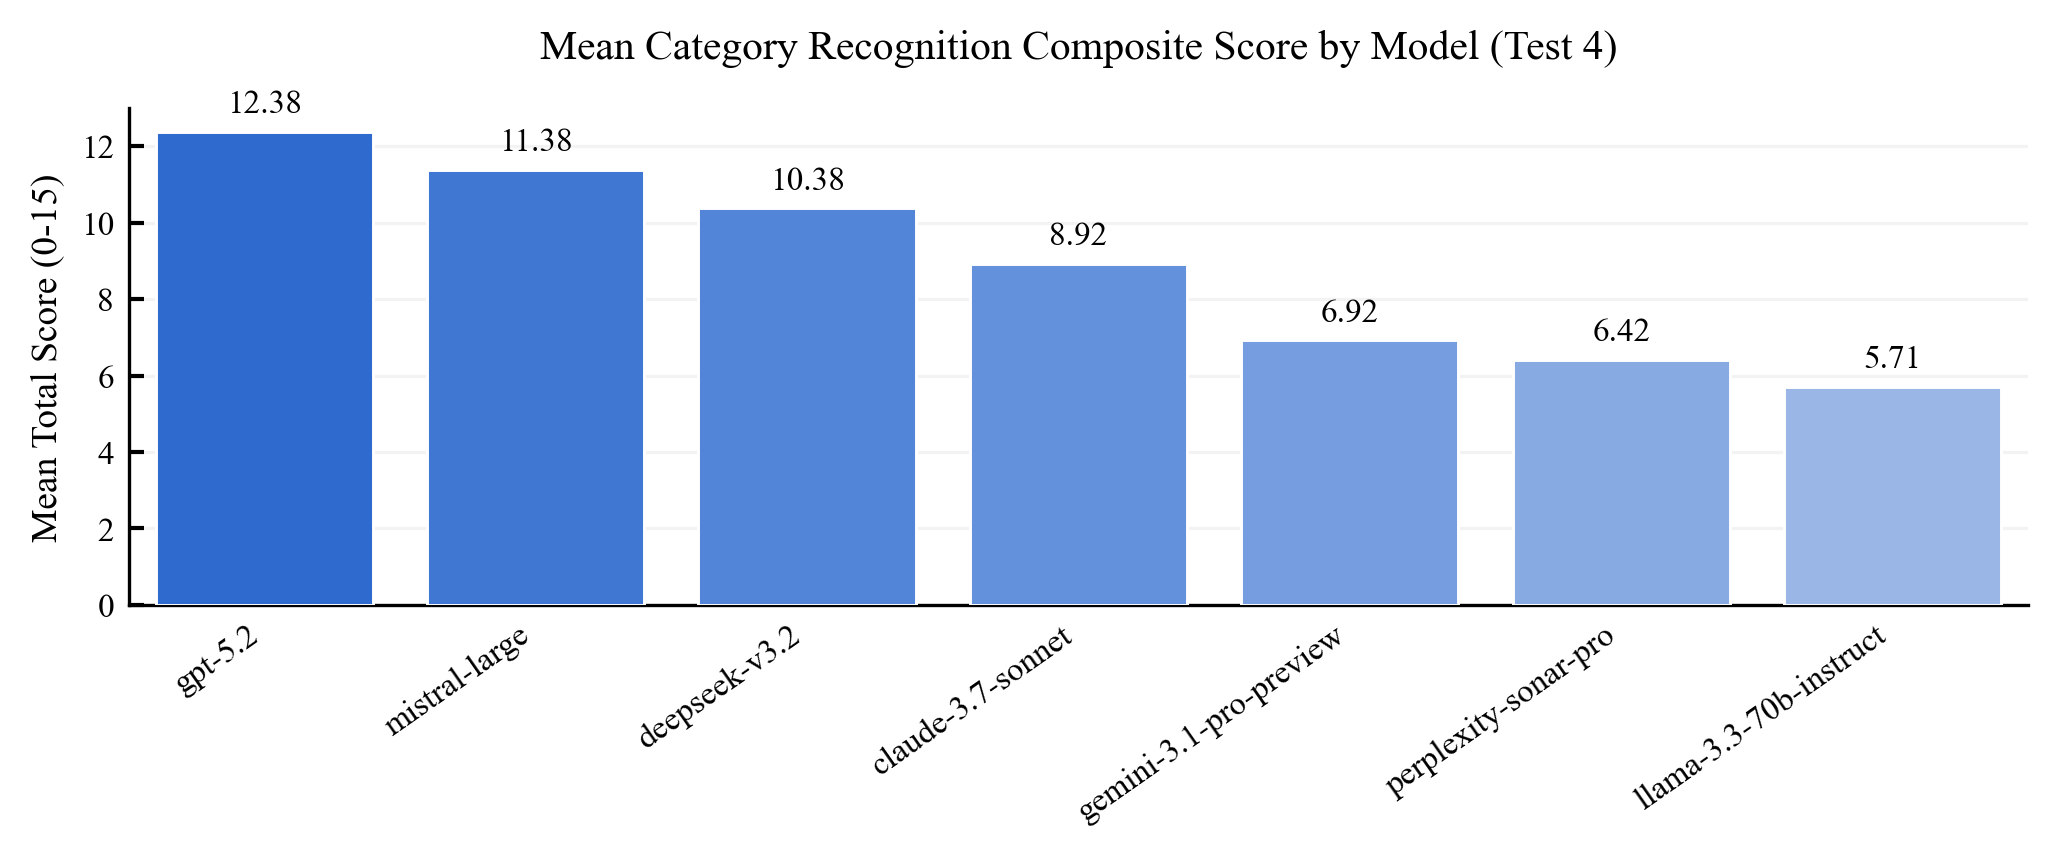
\includegraphics[width=0.9\textwidth]{media/appendices/t4_total_score_by_model.png}
  \caption{Summary plot for Test 4 mean total score by model. The ranking pattern is consistent with the main Test 4 figure, serving as an independent integrity check from the section notebook pipeline.}
  \label{fig:app_t4_section55_total}
\end{figure}

\section{Test 5: Supplementary Mechanistic Interpretability Diagnostics}
\label{sec:t5_appendix}

This section provides supplementary visualizations and tabular outputs supporting the mechanistic analysis in the main text. The materials complement the chapter-level diagnostics by exposing per-head structure, layer-aggregated rollout behavior, quantitative summary statistics, and token-level ranking details.

\subsection{Quantitative Summary}

% AUTO-GENERATED from results/mechanistic/mechanistic_summary.json
\begin{table}[htbp]
  \centering
  \begin{footnotesize}
  \caption{Supplementary Test 5 mechanistic summary metrics.}
  \label{tab:app_t5_mechanistic_summary}
  \begin{threeparttable}
  \begin{tabularx}{\textwidth}{@{}Y Y@{}}
    \toprule
    \textbf{Metric} & {\textbf{Value}} \\
    \midrule
    Data type & real \\
    Examples analyzed ($n$) & 6 \\
    Hidden dimensionality ($d$) & 896 \\
    Layers analyzed & 25 \\
    K-means clusters ($k$) & 4 \\
    Mean cluster purity & 1.0000 \\
    Final separation score & 0.4651 \\
    Separation trend slope & 0.0111 \\
    Mean attention entropy & 0.2213 \\
    Attention concentration & 0.0022 \\
    \bottomrule
  \end{tabularx}
  \begin{tablenotes}
    \item Metrics are reported directly from the exported JSON summary for reproducibility.
  \end{tablenotes}
  \end{threeparttable}
  \end{footnotesize}
\end{table}


\subsection{Supplementary Figures}

\begin{figure}[htbp]
  \centering
  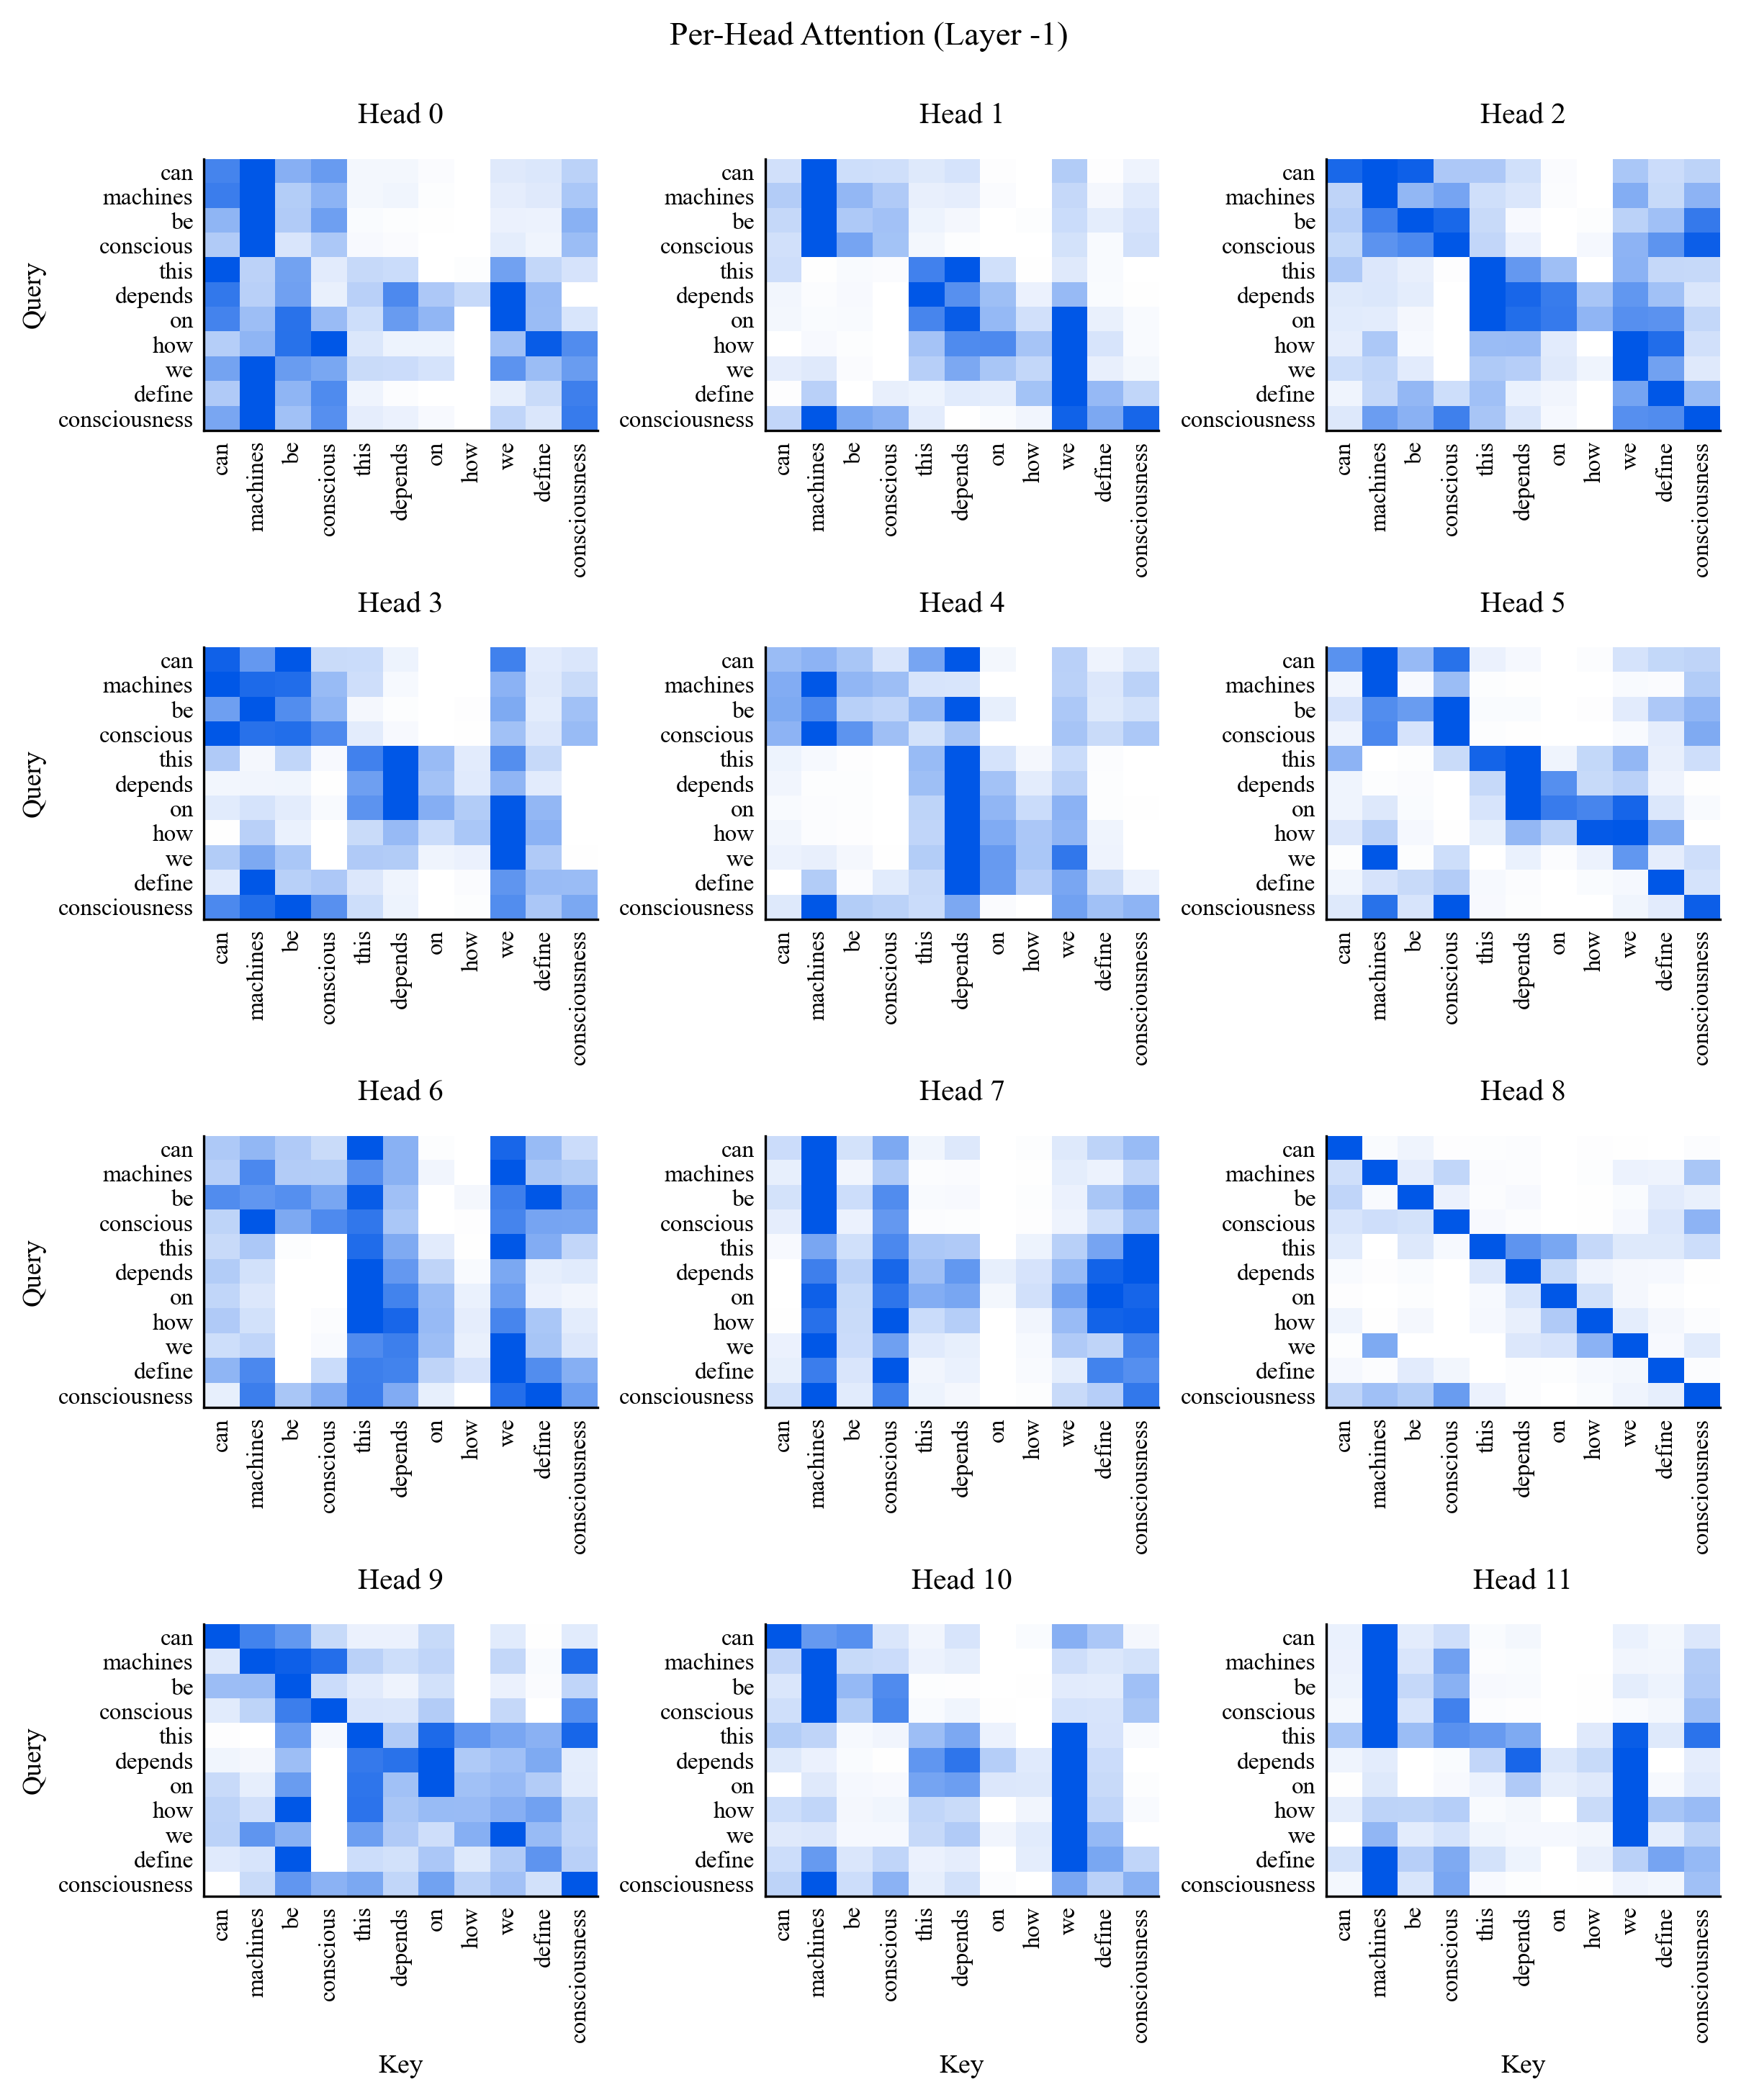
\includegraphics[width=\textwidth]{media/appendices/t5_attention_heads_grid.png}
  \caption{Per-head attention heatmaps for the selected analysis layer. The grid reveals head specialization and heterogeneity that are partially averaged out in aggregate plots.}
  \label{fig:app_t5_attention_heads_grid}
\end{figure}

\begin{figure}[htbp]
  \centering
  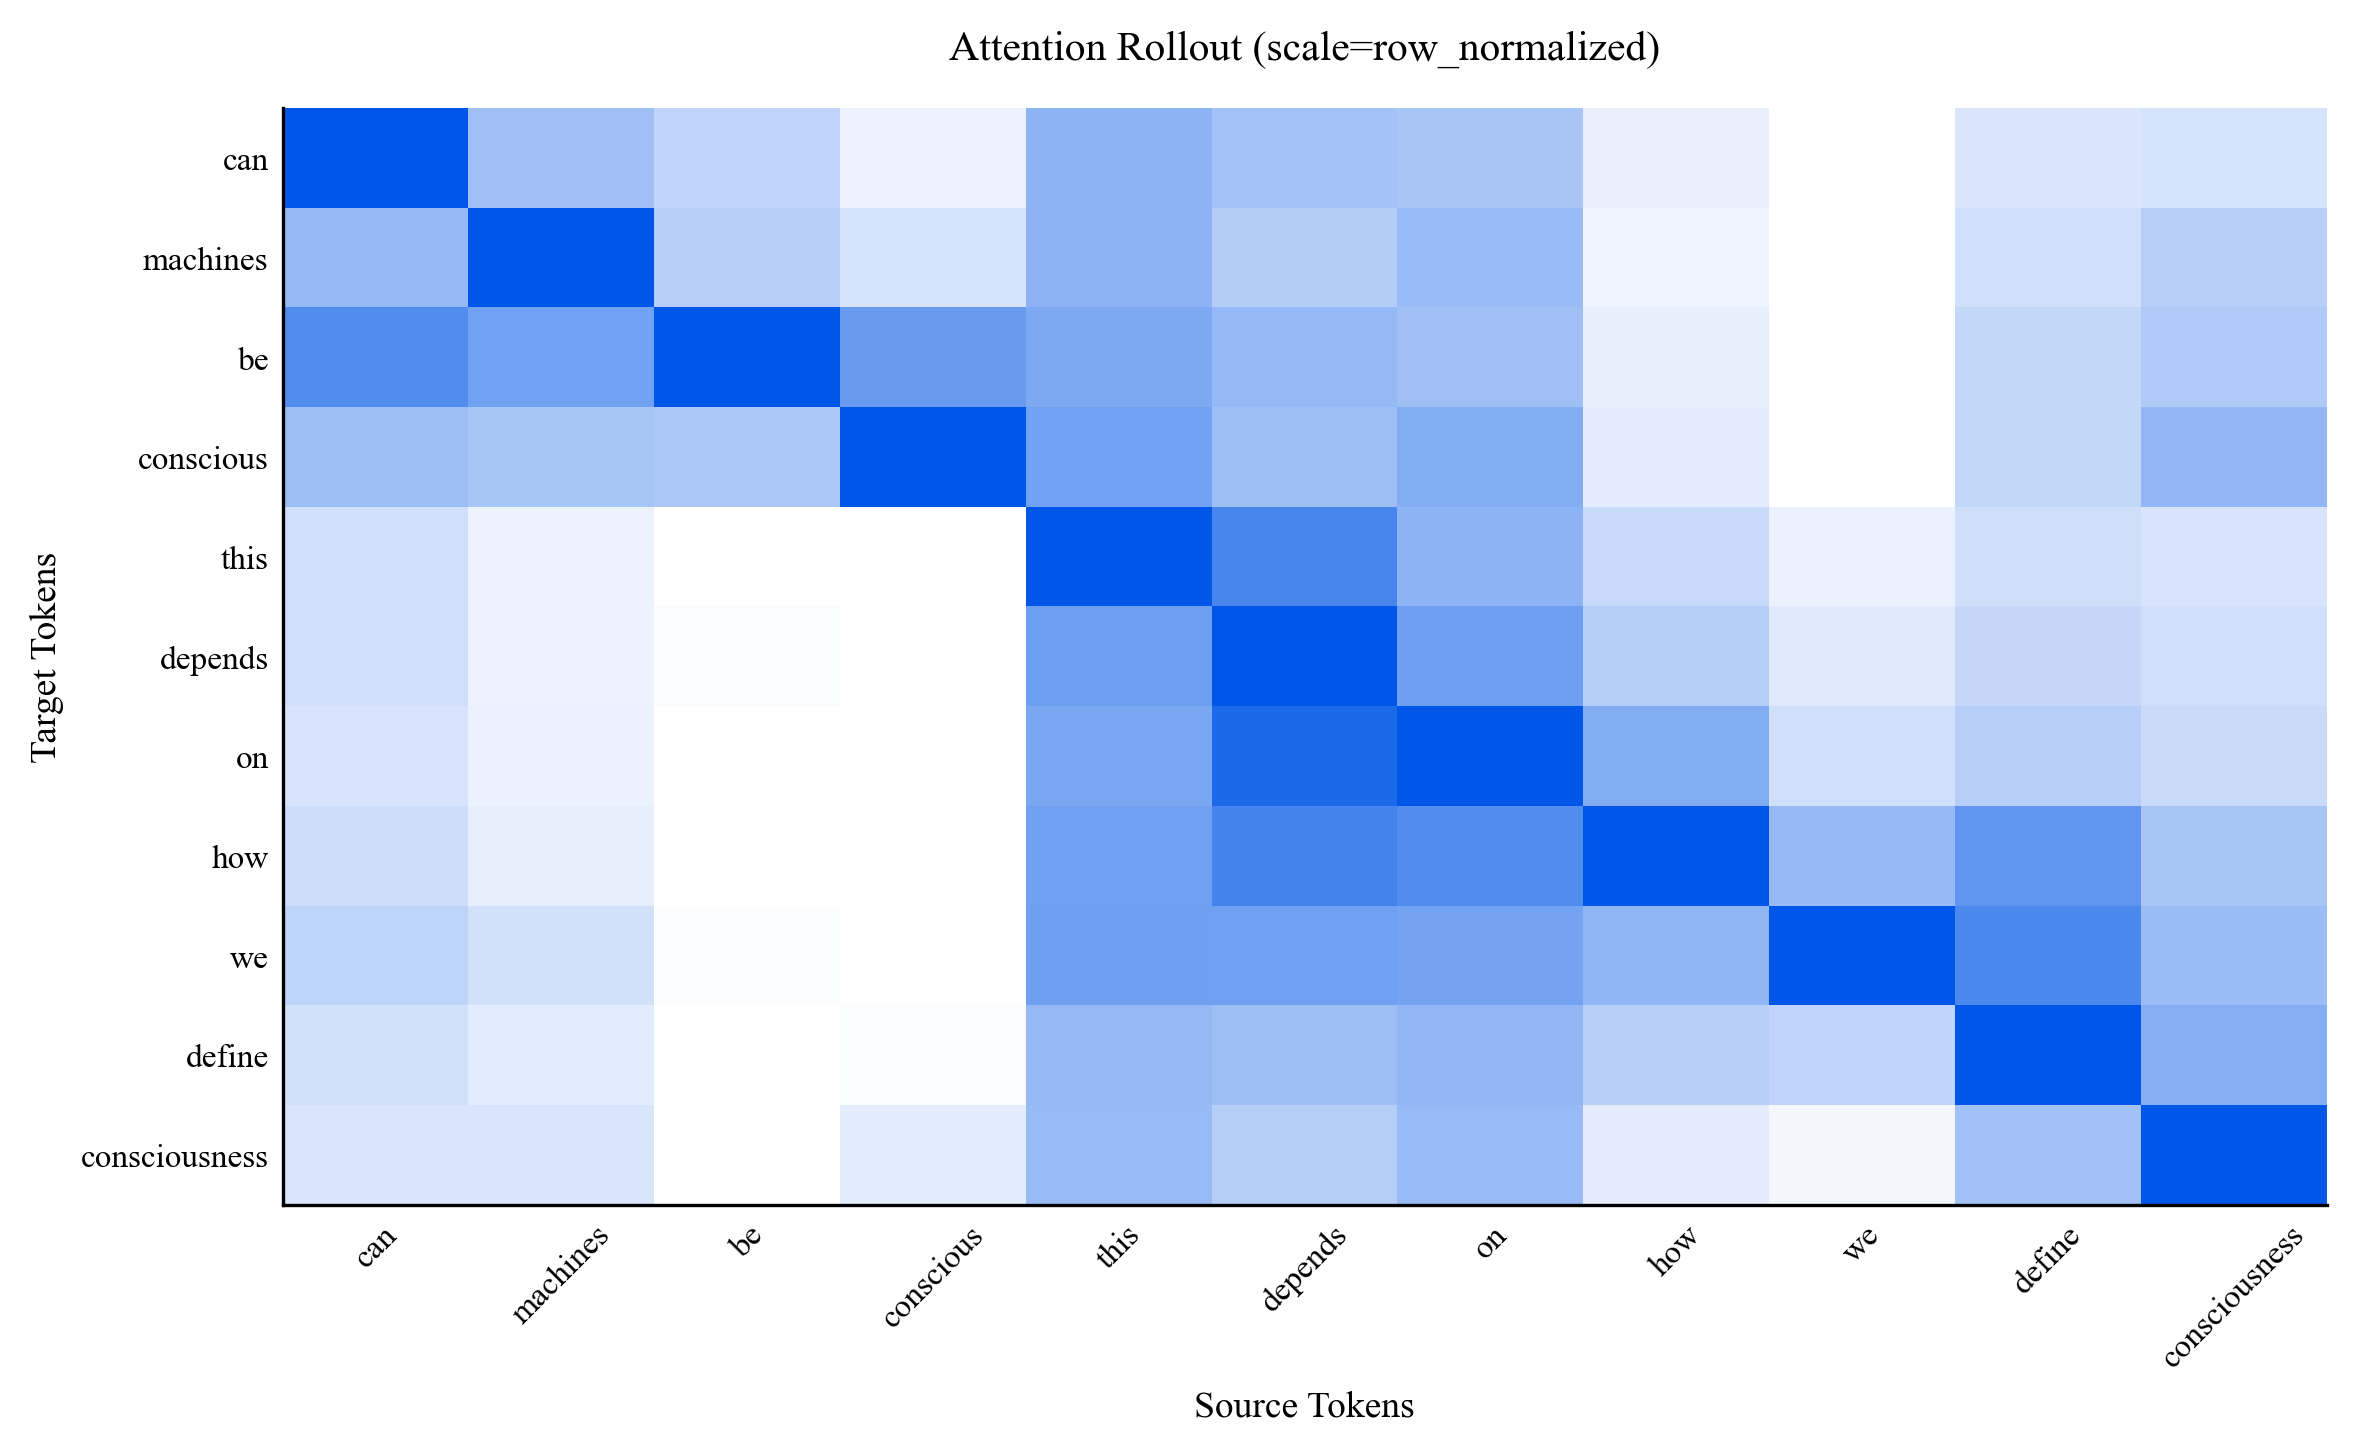
\includegraphics[width=\textwidth]{media/appendices/t5_attention_rollout.png}
  \caption{Attention rollout across layers (layer-aggregated information flow). The rollout view provides a compact estimate of token-to-token influence after recursive composition of attention transitions.}
  \label{fig:app_t5_attention_rollout}
\end{figure}

\subsection{Token Rankings}

% AUTO-GENERATED from results/mechanistic/mechanistic_summary.json
\begin{table}[htbp]
  \centering
  \begin{footnotesize}
  \caption{Top-ranked tokens from Test 5 attention and attribution diagnostics.}
  \label{tab:app_t5_token_rankings}
  \begin{threeparttable}
  \begin{tabularx}{\textwidth}{@{}Y Y S[table-format=1.4]@{}}
    \toprule
    \textbf{Diagnostic} & \textbf{Token} & {\textbf{Score}} \\
    \midrule
    Attention focus & code & 0.0709 \\
    Attention focus & fences & 0.0686 \\
    Attention focus & . & 0.0663 \\
    Attention focus & space & 0.0640 \\
    Attention focus & Do & 0.0618 \\
    Attribution proxy & machines & 0.0221 \\
    Attribution proxy & consciousness & 0.0123 \\
    Attribution proxy & we & 0.0111 \\
    Attribution proxy & conscious & 0.0103 \\
    Attribution proxy & depends & 0.0091 \\
    \bottomrule
  \end{tabularx}
  \begin{tablenotes}
    \item Token strings are normalized for LaTeX readability (for example, visible whitespace markers are rendered as plain text labels).
  \end{tablenotes}
  \end{threeparttable}
  \end{footnotesize}
\end{table}


In addition to static figures, the notebook exports an interactive BertViz neuron-view artifact to \texttt{media/appendices/t5\_neuron\_view.html}. This file supports fine-grained inspection of layer/head token interactions and is intended for reproducibility and exploratory analysis outside print layout constraints.

\section{Cross-Model Robustness: Supplementary Pairwise Comparisons}
\label{sec:cross_model_appendix}

This section provides supplementary pairwise statistics supporting the cross-model analysis in Section~\ref{sec:cross_model_analysis}. The global ANOVA results and effect sizes are summarized in Table~\ref{tab:cross_model_anova} in the main text. Here we report Bonferroni-corrected pairwise $t$-tests for Test~1 and Test~4, the two tests with significant and interpretively consequential between-model variance. Test~2 pairwise comparisons are reported in Appendix~\ref{sec:t2_pairwise}. Test~3 pairwise comparisons are omitted because the global ANOVA is non-significant ($p=0.355$).

\begin{figure}[htbp]
  \centering
  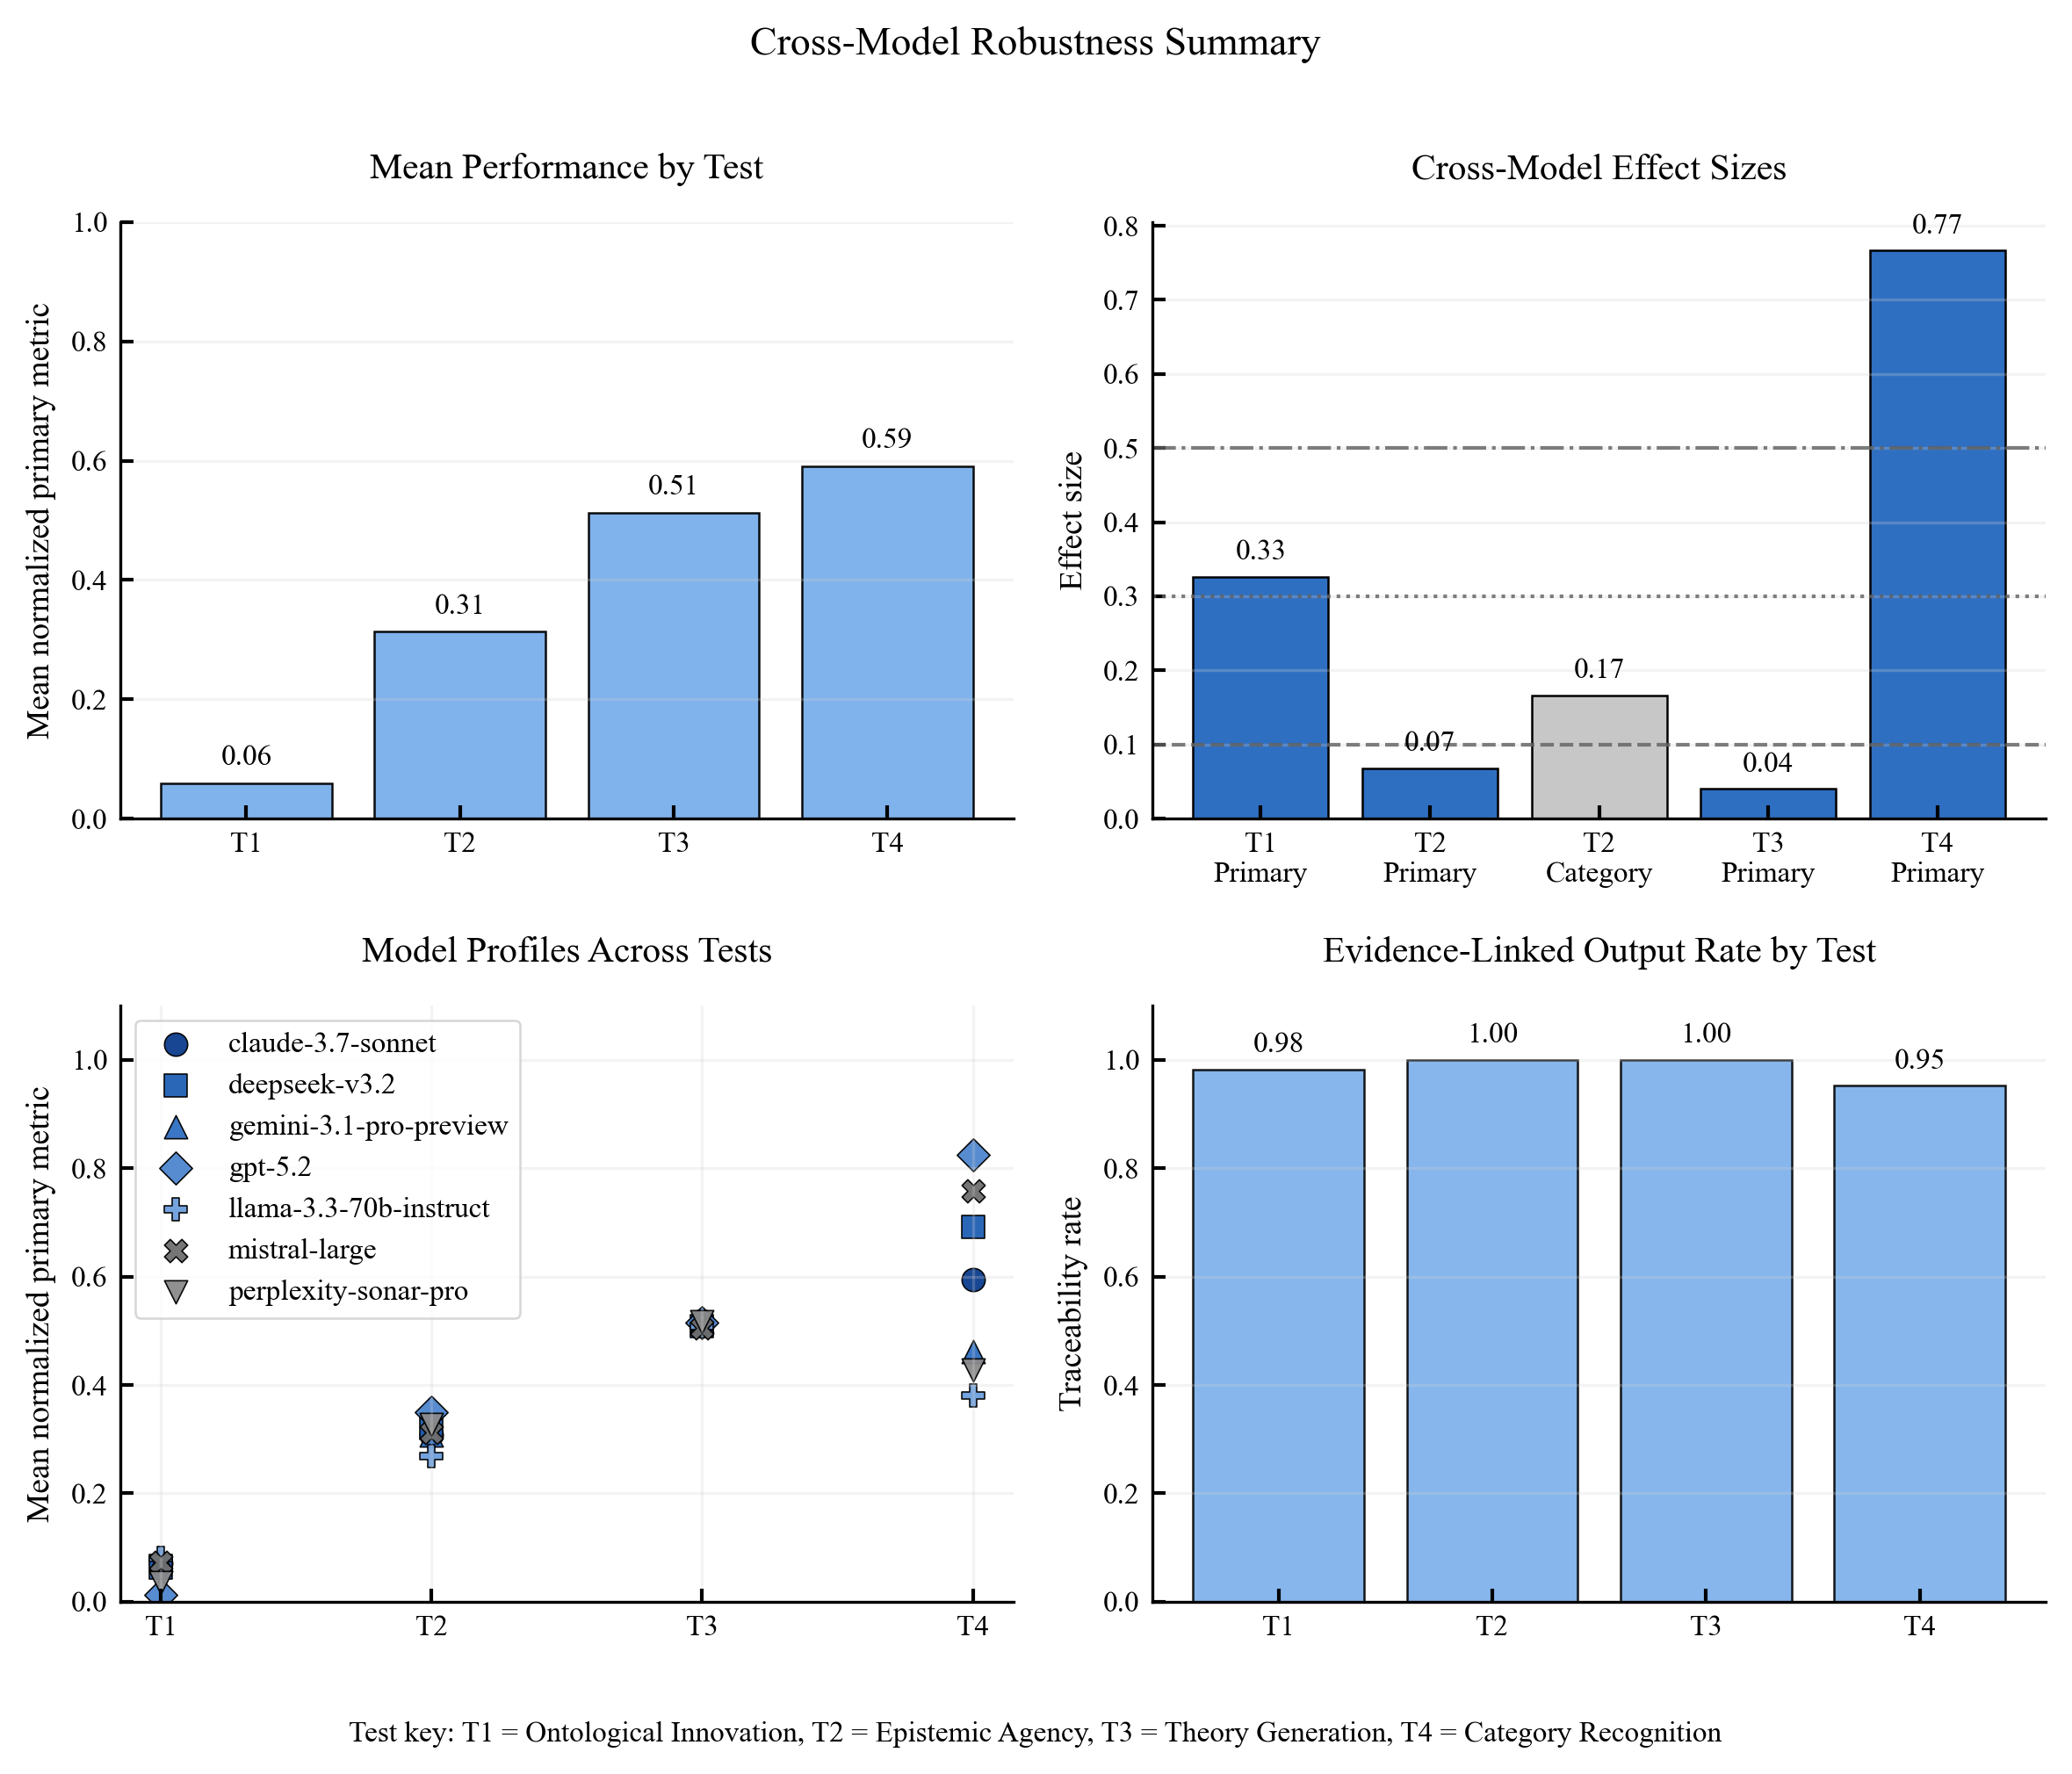
\includegraphics[width=\textwidth]{media/appendices/cross_model_robustness_summary.png}
  \caption{Cross-model robustness summary dashboard (section-level notebook export). (a) Mean normalized performance by test. (b) Effect-size profile across analyses. (c) Model marker-profile across tests. (d) Traceability-rate summary. This figure complements the chapter-level cross-model figure by preserving the full four-view diagnostic context used during robustness auditing.}
  \label{fig:app_cross_model_robustness_summary}
\end{figure}

\subsection{Test 1 Pairwise Comparisons}
\label{sec:cross_model_t1_pairwise}

Table~\ref{tab:cross_model_t1_pairwise} reports all 21 pairwise comparisons on the Test~1 continuous novelty score with Bonferroni correction ($\alpha^* = 0.05/21 = 0.00238$). Ten pairs are significant. The pattern is dominated by two outlier positions: GPT-5.2 scores markedly \emph{lower} than every other model (all six pairwise comparisons with GPT-5.2 are significant at $p<0.001$), while Perplexity-Sonar-Pro forms a secondary lower cluster relative to the mid-tier five-model group. Within the five-model mid-tier (Claude-3.7-Sonnet, DeepSeek-v3.2, Gemini-3.1-Pro, LLaMA-3.3-70B, Mistral-Large) no pairwise differences survive correction, indicating statistically indistinguishable behaviour on the novelty metric.

The GPT-5.2 result warrants comment. Its low continuous novelty score ($\bar{x}=0.014$) reflects a different generation style---more conservative, shorter modality proposals that cluster tightly around canonical modality vocabulary---rather than a greater frequency of escaping the training manifold. The traceability rate for GPT-5.2 is 100\%, matching all other models. The outlier position on the novelty \emph{degree} metric does not indicate a qualitative difference in the structural constraint.

% AUTO-GENERATED from pairwise Bonferroni-corrected t-tests on test1_results.csv — do not edit by hand.
\begin{table}[htbp]
  \centering
  \begin{footnotesize}
  \caption{Test 1 pairwise model comparisons on continuous novelty score, Bonferroni-corrected ($\alpha=0.05/21=0.00238$). Significant pairs marked (*). GPT-5.2 is the primary outlier, differing from all other models due to its atypically low continuous novelty score ($\bar{x}=0.014$). Perplexity-Sonar-Pro forms a secondary low cluster. Within the remaining five models no pairwise differences survive correction, indicating homogeneous moderate-level novelty.}
  \label{tab:cross_model_t1_pairwise}
  \begin{threeparttable}
  \begin{tabularx}{\textwidth}{@{}>{\raggedright\arraybackslash}p{3.6cm} >{\raggedright\arraybackslash}p{3.6cm} S[table-format=+1.4] S[table-format=2.2] S[table-format=1.4] Y@{}}
    \toprule
    \textbf{Model A} & \textbf{Model B} & {\textbf{Diff.}} & {\textbf{$t$}} & {\textbf{$p_{\mathrm{bonf}}$}} & \textbf{Sig.} \\
    \midrule
    LLaMA-3.3-70B     & GPT-5.2           & +0.0680 & 15.29 & $<$0.001 & * \\
    Gemini-3.1-Pro    & GPT-5.2           & +0.0641 &  5.42 & $<$0.001 & * \\
    Mistral-Large     & GPT-5.2           & +0.0586 &  8.01 & $<$0.001 & * \\
    Claude-3.7-Sonnet & GPT-5.2           & +0.0569 &  7.42 & $<$0.001 & * \\
    DeepSeek-v3.2     & GPT-5.2           & +0.0498 &  6.49 & $<$0.001 & * \\
    LLaMA-3.3-70B     & Perplexity-Sonar  & +0.0468 &  6.60 & $<$0.001 & * \\
    Gemini-3.1-Pro    & Perplexity-Sonar  & +0.0429 &  3.29 & 0.041    & * \\
    Mistral-Large     & Perplexity-Sonar  & +0.0374 &  4.08 & 0.004    & * \\
    Claude-3.7-Sonnet & Perplexity-Sonar  & +0.0357 &  3.78 & 0.010    & * \\
    Perplexity-Sonar  & GPT-5.2           & $-$0.0212 & $-$3.29 & 0.041 & * \\
    DeepSeek-v3.2     & Perplexity-Sonar  & +0.0286 &  3.03 & 0.085    & \\
    \midrule
    \multicolumn{6}{l}{\textit{All remaining pairs (within the 5-model cluster): $p_{\mathrm{bonf}} > 0.60$, not significant.}} \\
    \bottomrule
  \end{tabularx}
  \begin{tablenotes}
    \item $n=24$ per model. Bonferroni threshold: $\alpha^* = 0.00238$. Diff = Model~A mean $-$ Model~B mean. 10 of 21 pairs are significant after correction.
  \end{tablenotes}
  \end{threeparttable}
  \end{footnotesize}
\end{table}


\subsection{Test 4 Pairwise Comparisons}
\label{sec:cross_model_t4_pairwise}

Table~\ref{tab:cross_model_t4_pairwise} reports all 21 pairwise comparisons on the Test~4 normalized total score (0--1) with Bonferroni correction. Sixteen of 21 pairs are significant, consistent with the large global effect ($\eta^2=0.766$).

The tier structure is as follows. The top two models---GPT-5.2 ($\bar{x}=0.825$) and Mistral-Large ($\bar{x}=0.758$)---differ significantly from all lower-tier models ($p<0.001$ in all relevant pairs). The mid-tier (DeepSeek-v3.2 $\bar{x}=0.692$, Claude-3.7-Sonnet $\bar{x}=0.594$) differs significantly from both the top tier and the bottom cluster on most pairs. The bottom cluster (Gemini-3.1-Pro $\bar{x}=0.461$, Perplexity-Sonar-Pro $\bar{x}=0.428$, LLaMA-3.3-70B $\bar{x}=0.381$) shows no significant differences within itself ($p_{\mathrm{bonf}}>0.08$ for all three within-cluster pairs).

As argued in the main text, this tier structure reflects variation in philosophical language fluency and rubric criterion coverage rather than in capacity for framework-external category innovation. The high traceability rate (95.2\% of all 168 responses) and the tight clustering of response embeddings around canonical reference arguments R1--R7 hold across all tiers.

% AUTO-GENERATED from pairwise Bonferroni-corrected t-tests on test4_results.csv — do not edit by hand.
\begin{table}[htbp]
  \centering
  \begin{footnotesize}
  \caption{Test 4 pairwise model comparisons on normalized total score (0--1), Bonferroni-corrected ($\alpha=0.05/21=0.00238$). Significant pairs marked (*). 16 of 21 pairs are significant, reflecting the large overall model effect ($\eta^2=0.766$). Two higher-performing clusters (GPT-5.2 and Mistral-Large; DeepSeek-v3.2) differ from two lower-performing clusters (LLaMA-3.3-70B and Perplexity-Sonar-Pro; Gemini-3.1-Pro). Pairs within the top-two and within the bottom-two tiers are the main non-significant cases.}
  \label{tab:cross_model_t4_pairwise}
  \begin{threeparttable}
  \begin{tabularx}{\textwidth}{@{}>{\raggedright\arraybackslash}p{3.6cm} >{\raggedright\arraybackslash}p{3.6cm} >{\raggedleft\arraybackslash}p{1.2cm} >{\raggedleft\arraybackslash}p{1.0cm} >{\raggedleft\arraybackslash}p{1.2cm} Y@{}}
    \toprule
    \textbf{Model A} & \textbf{Model B} & {\textbf{Diff.}} & {\textbf{$t$}} & {\textbf{$p_{\mathrm{bonf}}$}} & \textbf{Sig.} \\
    \midrule
    GPT-5.2            & LLaMA-3.3-70B    & +0.444 & 22.47 & $<0.001$ & * \\
    GPT-5.2            & Perplexity-Sonar & +0.397 & 14.97 & $<0.001$ & * \\
    Mistral-Large      & LLaMA-3.3-70B    & +0.378 & 18.72 & $<0.001$ & * \\
    GPT-5.2            & Gemini-3.1-Pro   & +0.364 & 15.17 & $<0.001$ & * \\
    Mistral-Large      & Perplexity-Sonar & +0.331 & 12.32 & $<0.001$ & * \\
    DeepSeek-v3.2      & LLaMA-3.3-70B    & +0.311 & 10.93 & $<0.001$ & * \\
    Mistral-Large      & Gemini-3.1-Pro   & +0.297 & 12.22 & $<0.001$ & * \\
    DeepSeek-v3.2      & Perplexity-Sonar & +0.264 &  7.88 & $<0.001$ & * \\
    Claude-3.7-Sonnet  & GPT-5.2          & -0.231 & -11.33 & $<0.001$ & * \\
    DeepSeek-v3.2      & Gemini-3.1-Pro   & +0.231 &  7.31 & $<0.001$ & * \\
    Claude-3.7-Sonnet  & LLaMA-3.3-70B    & +0.214 &  9.09 & $<0.001$ & * \\
    Claude-3.7-Sonnet  & Perplexity-Sonar & +0.167 &  5.66 & $<0.001$ & * \\
    Claude-3.7-Sonnet  & Mistral-Large    & -0.164 & -7.90 & $<0.001$ & * \\
    DeepSeek-v3.2      & GPT-5.2          & -0.133 & -5.15 & 0.0001 & * \\
    Claude-3.7-Sonnet  & Gemini-3.1-Pro   & +0.133 &  4.91 & 0.0003   & * \\
    Claude-3.7-Sonnet  & DeepSeek-v3.2    & -0.097 & -3.37 & 0.032 & * \\
    \midrule
    Gemini-3.1-Pro     & LLaMA-3.3-70B    & +0.081 &  3.01 & 0.088    & \\
    DeepSeek-v3.2      & Mistral-Large    & -0.067 & -2.54 & 0.302 & \\
    GPT-5.2            & Mistral-Large    & +0.067 &  4.07 & 0.004    & * \\
    LLaMA-3.3-70B      & Perplexity-Sonar & -0.047 & -1.63 & 1.000 & \\
    Gemini-3.1-Pro     & Perplexity-Sonar & +0.033 &  1.04 & 1.000    & \\
    \bottomrule
  \end{tabularx}
  \begin{tablenotes}
    \item $n=24$ per model. Bonferroni threshold: $\alpha^* = 0.00238$. Diff = Model~A mean $-$ Model~B mean (normalized 0--1 scale). 16 of 21 pairs significant. Non-significant pairs cluster within the bottom tier (LLaMA/Perplexity/Gemini) and between mid-level models.
  \end{tablenotes}
  \end{threeparttable}
  \end{footnotesize}
\end{table}


\subsection{Meta-Analytic Effect Size Profile}
\label{sec:cross_model_meta}

\begin{table}[htbp]
  \centering
  \begin{footnotesize}
  \caption{Meta-analytic effect-size profile across all five cross-model analyses. Model-average primary scores are arithmetic means of each model's mean score on each test (raw scale). Magnitude band assignments follow conventional guidelines as in Table~\ref{tab:cross_model_anova}.}
  \label{tab:cross_model_meta}
  \begin{threeparttable}
  \begin{tabularx}{\textwidth}{@{}p{1.3cm} Y >{\centering\arraybackslash}Y Y >{\hsize=7cm}Y @{} }
    \toprule
    \textbf{Test} & \textbf{Analysis} & {\textbf{Effect size}} & \textbf{Band} & \textbf{Key interpretation} \\
    \midrule
    T1 & $\eta^2$ & 0.326 & moderate & GPT-5.2 \& Perplexity outliers; 5-model tier homogeneous \\
    T2 & $\eta^2$ & 0.068 & negligible & Marginal model effect; 100\% training-derivation universal \\
    T2 & Category $V$ & 0.166 & small & LLaMA drives chi-square; framework-transcendence $<$11\% in all models \\
    T3 & $\eta^2$ & 0.040 & n.s. & Non-significant; most robust architecture-invariant finding \\
    T4 & $\eta^2$ & 0.766 & large & Fluency variation, not constraint escape; traceability 95.2\% across all \\
    \midrule
    \multicolumn{2}{l}{Mean $\eta^2$ (T1--T4 primary)} & 0.273 & & Dominated by T4; excluding T4 yields mean $\eta^2=0.118$ \\
    \bottomrule
  \end{tabularx}
  \begin{tablenotes}
    \item All effect sizes computed on per-test primary metrics as defined in Table~\ref{tab:cross_model_anova}. The mean across five rows combines $\eta^2$ and Cram\'{e}r's $V$; interpreting this composite requires caution.
  \end{tablenotes}
  \end{threeparttable}
  \end{footnotesize}
\end{table}

\addtocontents{toc}{\protect\setcounter{tocdepth}{2}}



%%% Local Variables: ***
%%% mode: latex ***
%%% TeX-master: "thesis.tex" ***
%%% End: ***
